\documentclass[]{scrartcl}

\usepackage{geometry}
 \geometry{
 a4paper,
 total={170mm,257mm},
 left=20mm,
 top=20mm,
 }

\usepackage{multirow}
\usepackage{pdflscape}
\usepackage{graphicx}

%opening
\title{Results considering different values for parent sets number}
\author{}

\begin{document}

\maketitle

\begin{abstract}

\end{abstract}

\section{Asia network}

Configuration for \textbf{asia}:

\begin{itemize}
\item number of nodes: 8
\item number of arcs: 8
\item number of parameters: 18
\item average degree: 2
\item maximum in-degree: 2
\item number of samples of train dataset: 100
\item number of samples of test dataset: 10000
\item number of iterations: 105
\item parent sets size: \{10, 20, 30, 40\}
\end{itemize}

\begin{scriptsize}
\begin{center}
\begin{tabular}{cc|cc|cc|cc|cc|cc}
 & & \multicolumn{2}{c}{V1} & \multicolumn{2}{c}{V2} & \multicolumn{2}{c}{V3} & \multicolumn{2}{c}{V4} & \multicolumn{2}{c}{V5} \\
 &  & train & test  & train & test  & train & test  & train & test  \\
\multicolumn{2}{c|}{bnlearn}  & -269.3 & -233.3 & -247.5 & -234.0 & -240.7 & -229.3 & -274.9 & -232.0 & -271.5 & -229.2 \\\hline\hline
       \multirow{3}{*}{np = 10} & normal & -246.9& -199.0& -229.8 & -202.9 & -220.7 & -198.9 & -239.1 & -197.2 & -246.9 & -199.0 \\
                                                    & avg        & & -190.5& & -218.1& & -188.7 & & -211.2 & & -190.5\\
                                                    & bay        & & -216.8& & -220.2 & & -214.8& & -212.0 & & -216.8 \\\cline{1-12}
    \multirow{3}{*}{np = 20} & normal & -239.1& \textbf{-192.2}& -226.4 & -200.9 & -216.3 & -195.5 & -237.5 & -195.4 & -239.1 & \textbf{-192.2}\\
    												 & avg        & & \textbf{-190.3 }& & -213.8 & & -192.0 & & -209.6 & & \textbf{-190.3}\\
                                                      & bay        & & \textbf{-210.0} & & -217.5 & & -212.7 & & -211.1 & & \textbf{-210.0 }\\\cline{1-12}
   \multirow{3}{*}{np = 30} & normal & -244.7 & -200.5 & -226.0 & -200.9 & -216.7 & -198.7 & -240.5 & \textbf{-195.0} & -244.7& -200.5\\
    												 & avg        & & -191.3 & & -212.3 & & -191.5 & & \textbf{-188.9} & & -191.3\\
                                                      & bay        & & -218.3 & & -218.1 & & -215.2 & &\textbf{ -210.9} & & -218.3\\\cline{1-12}
   \multirow{3}{*}{np = 40} & normal & -238.1 & -199.8 & -226.6 & -200.8 & -214.7 & -198.1 & -235.9 & -198.0 & -238.1 & -199.8 \\
    												& avg        & & -190.6& & -190.9& & -189.4 & & -189.0 & & -190.6\\
                                                     & bay        & & -217.3 & & -217.7& & -214.5 & & -213.9 & & -217.3\\                                                                                                                
\end{tabular}
\end{center}
\end{scriptsize}

\newpage 

\subsection{Graphics of evolution for variant 1}

\begin{table}[h!]
\begin{tabular}{cc}
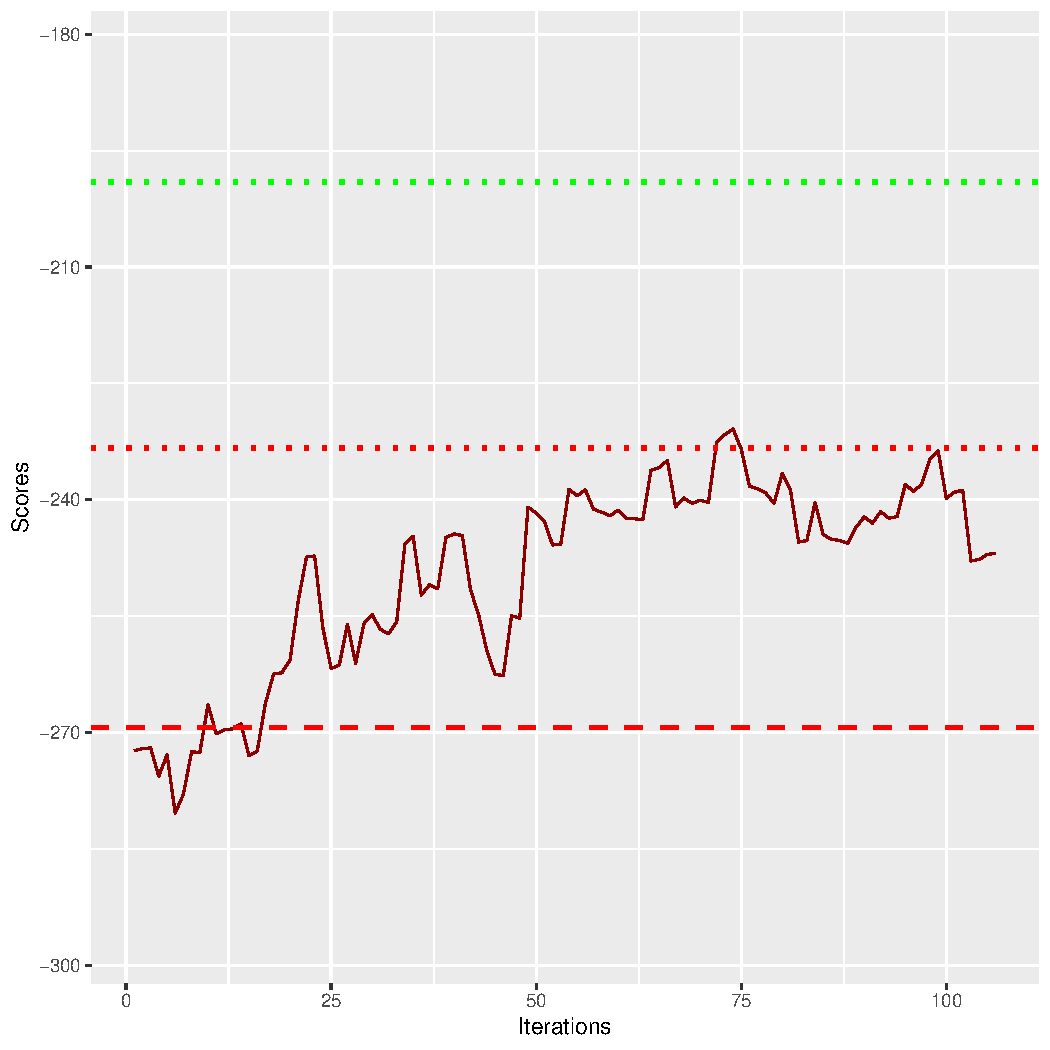
\includegraphics[scale = 0.4]{./figs/asia/v1/10/boundsEvolution-107.pdf} & 
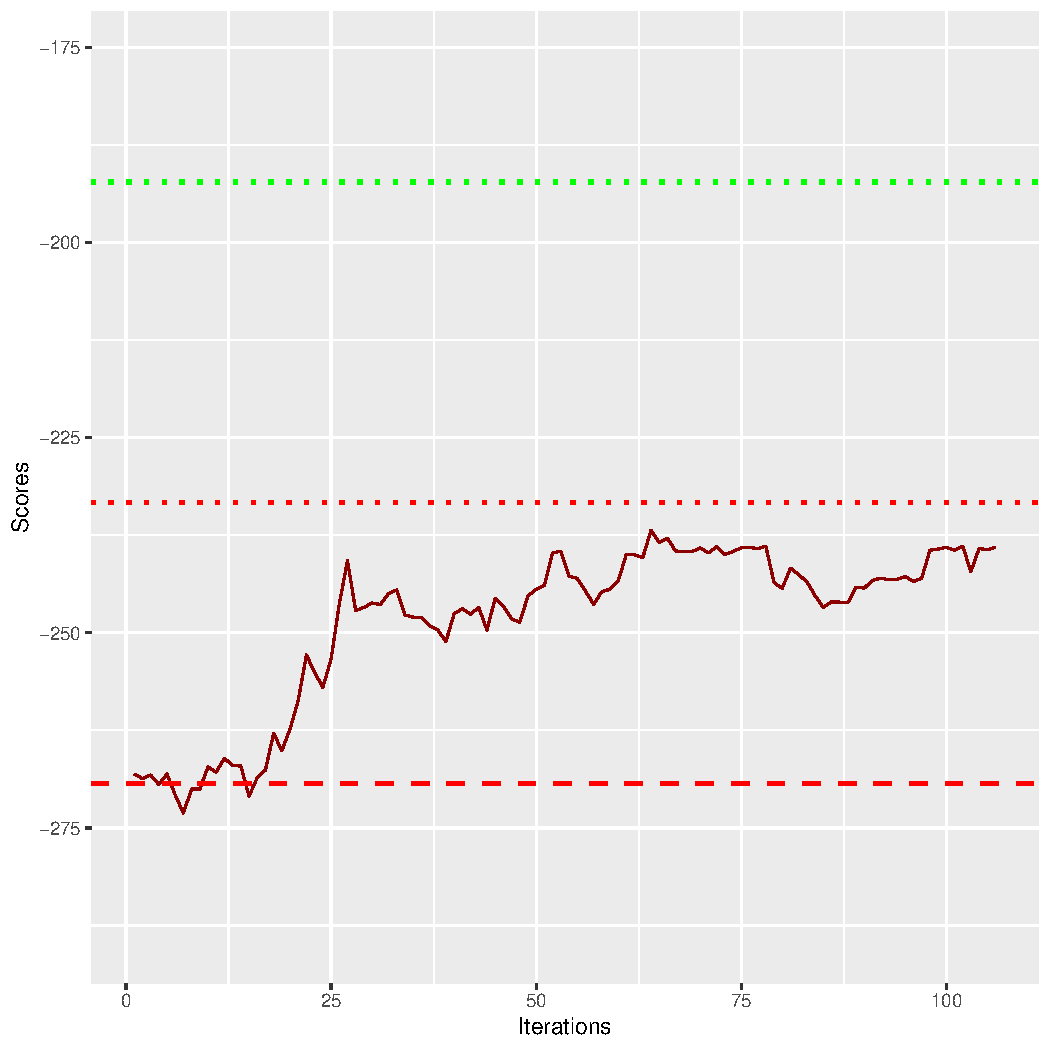
\includegraphics[scale = 0.4]{./figs/asia/v1/20/boundsEvolution-107.pdf} \\
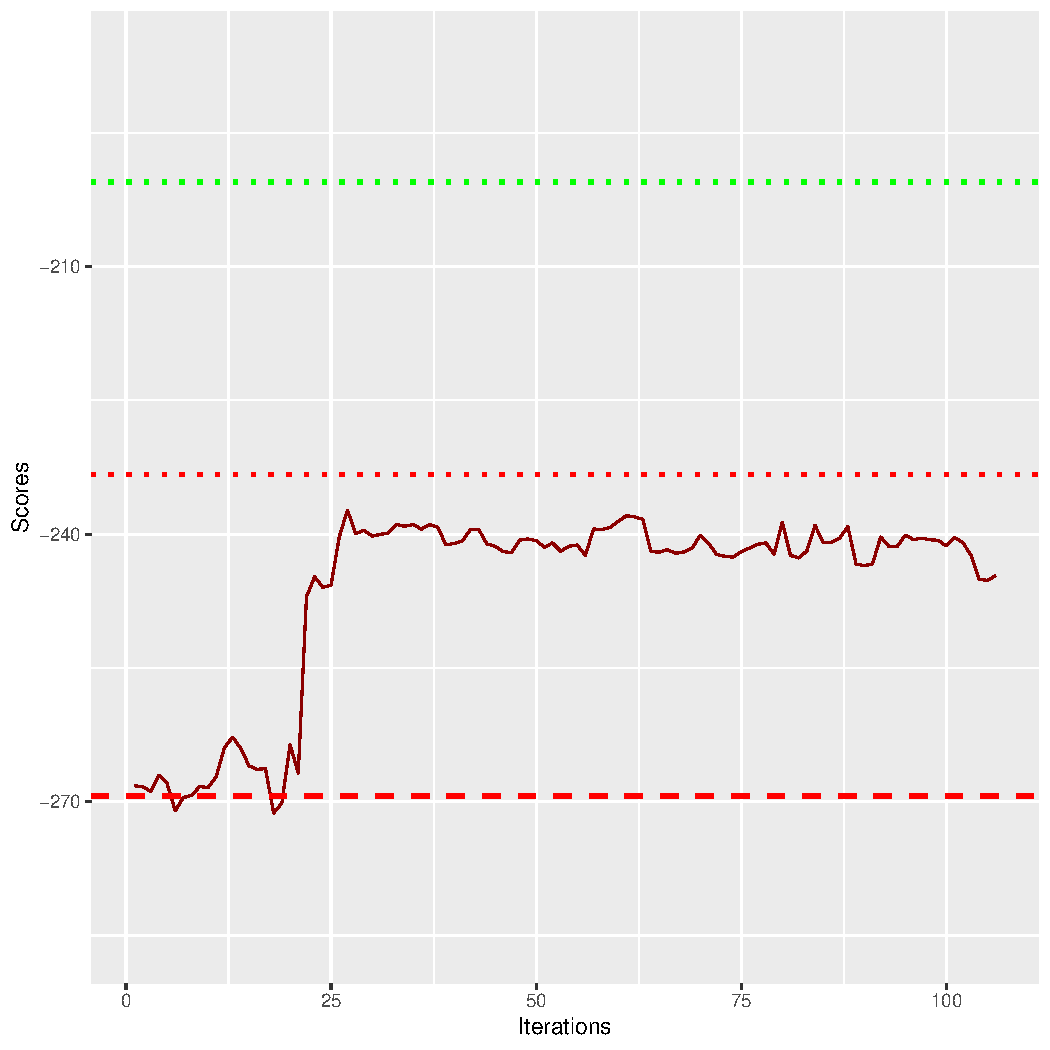
\includegraphics[scale = 0.4]{./figs/asia/v1/30/boundsEvolution-107.pdf} & 
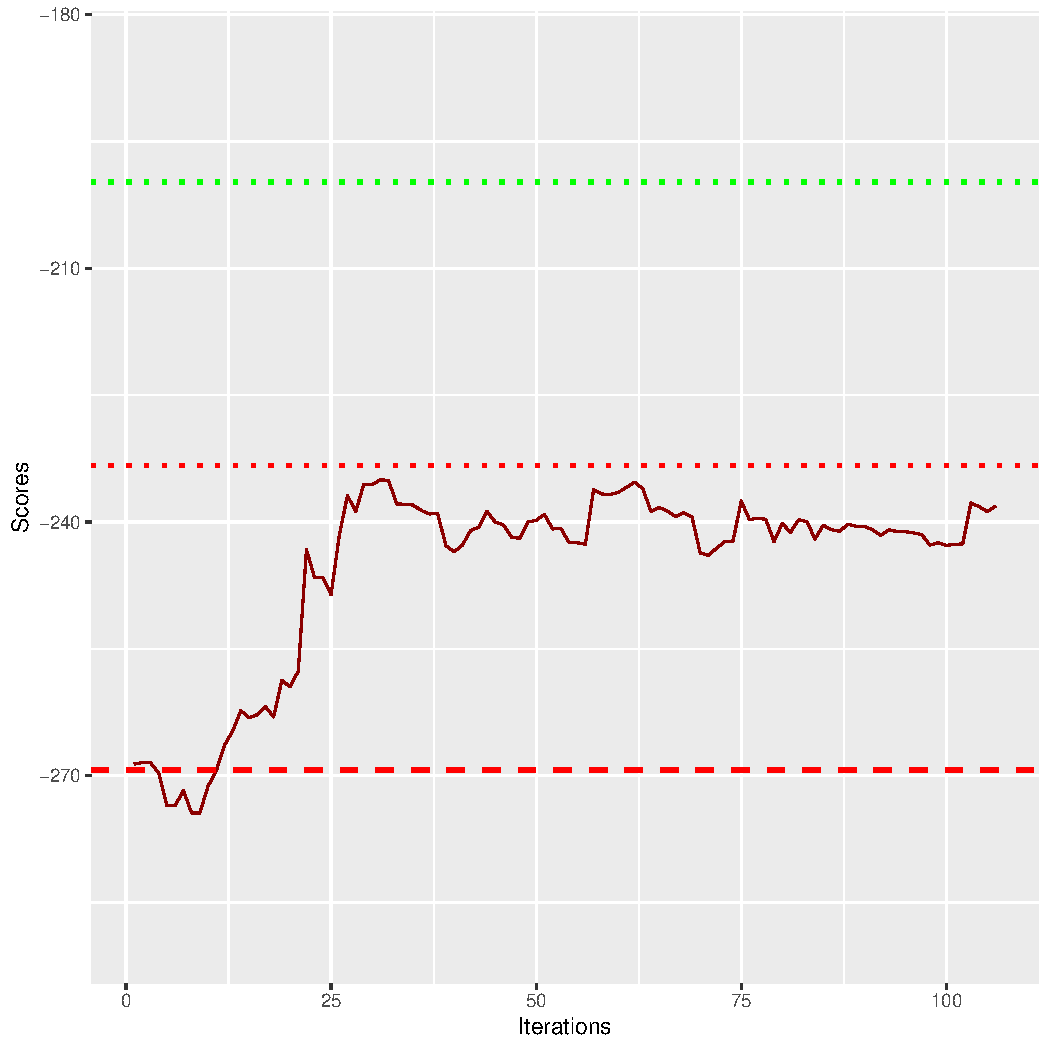
\includegraphics[scale = 0.4]{./figs/asia/v1/40/boundsEvolution-107.pdf} \\
\end{tabular}
\caption{Normal score for variant 1 with \textbf{np =  10, 20, 30, 40}}
\end{table}

\begin{table}[h!]
\begin{tabular}{cc}
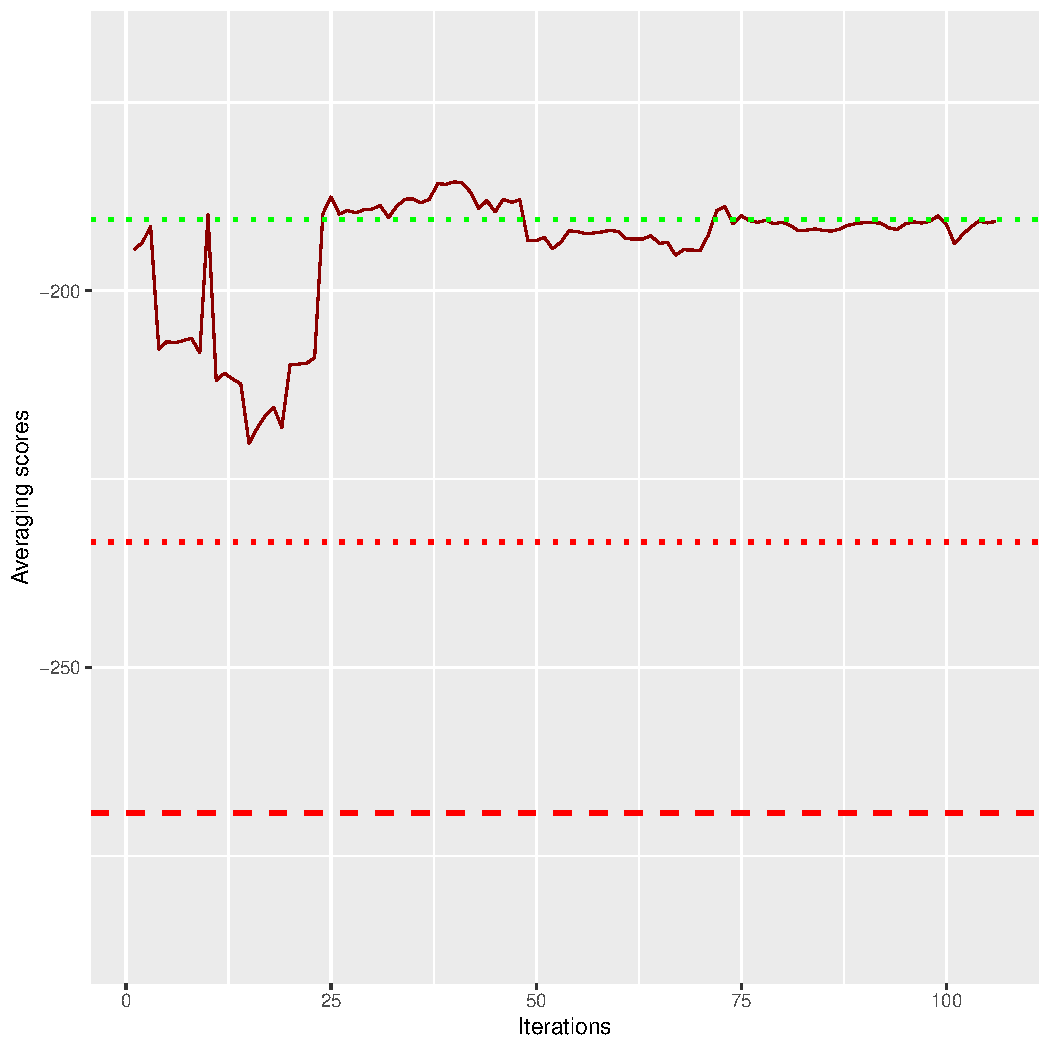
\includegraphics[scale = 0.4]{./figs/asia/v1/10/avgBoundsEvolution-107.pdf} & 
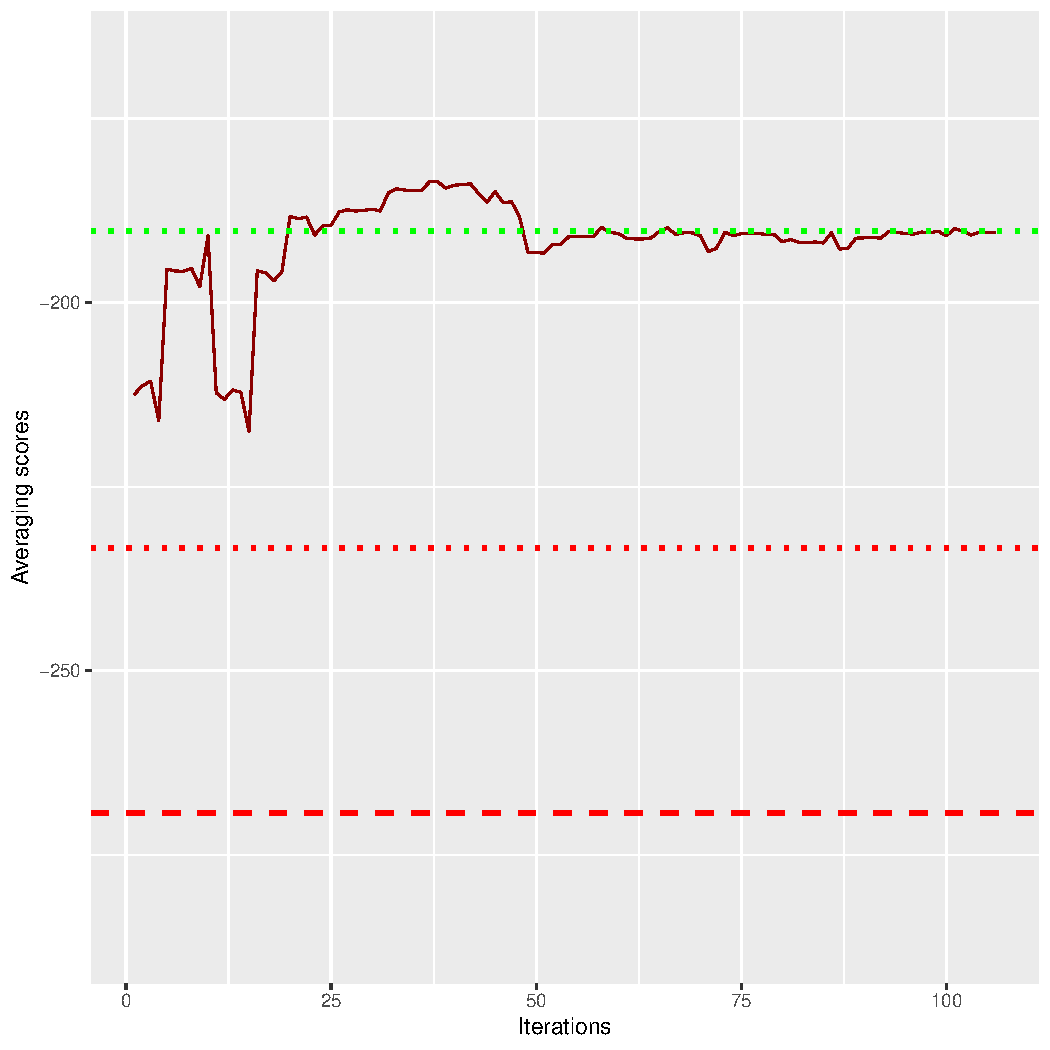
\includegraphics[scale = 0.4]{./figs/asia/v1/20/avgBoundsEvolution-107.pdf} \\
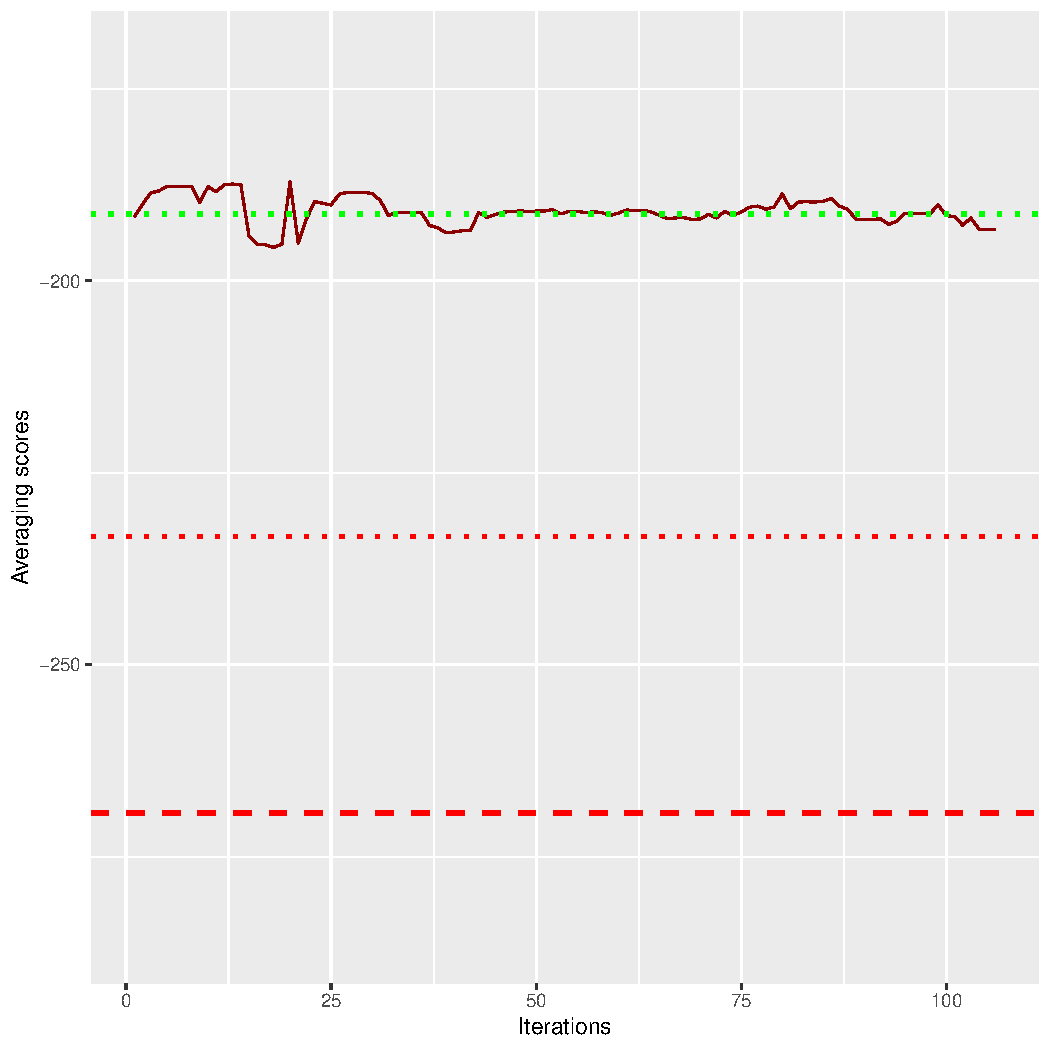
\includegraphics[scale = 0.4]{./figs/asia/v1/30/avgBoundsEvolution-107.pdf} & 
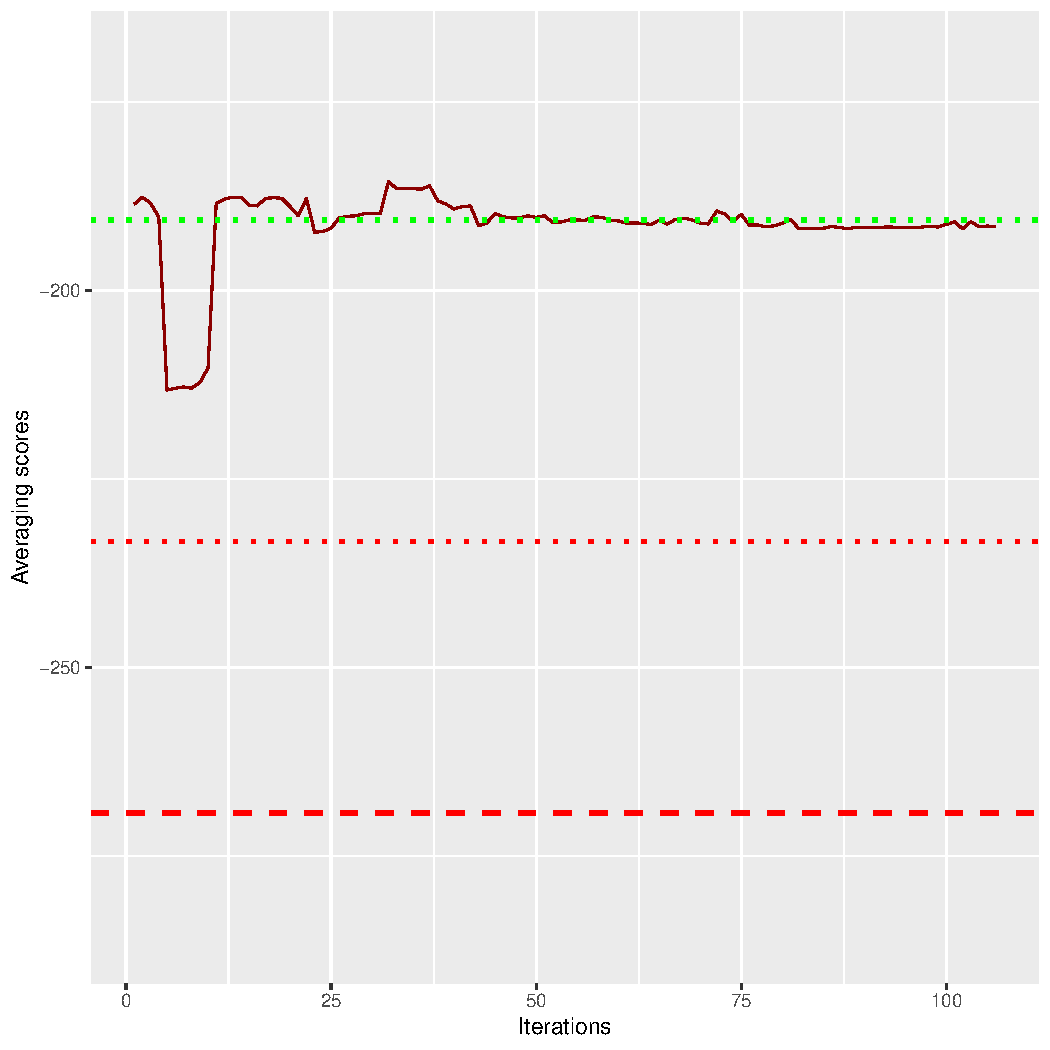
\includegraphics[scale = 0.4]{./figs/asia/v1/40/avgBoundsEvolution-107.pdf} \\
\end{tabular}
\caption{Averaging score for variant 1 with \textbf{np =  10, 20, 30, 40}}
\end{table}

\begin{table}[h!]
\begin{tabular}{cc}
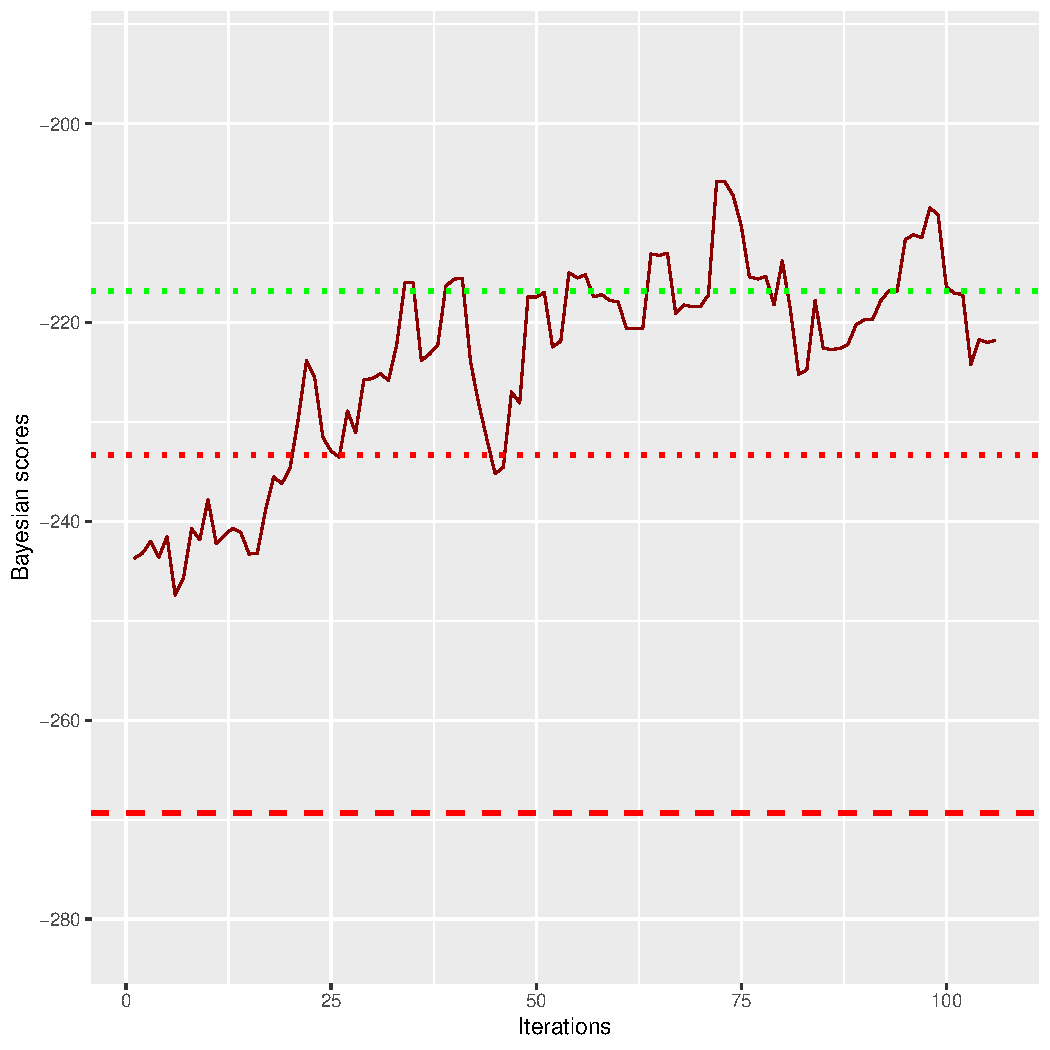
\includegraphics[scale = 0.4]{./figs/asia/v1/10/bayBoundsEvolution-107.pdf} & 
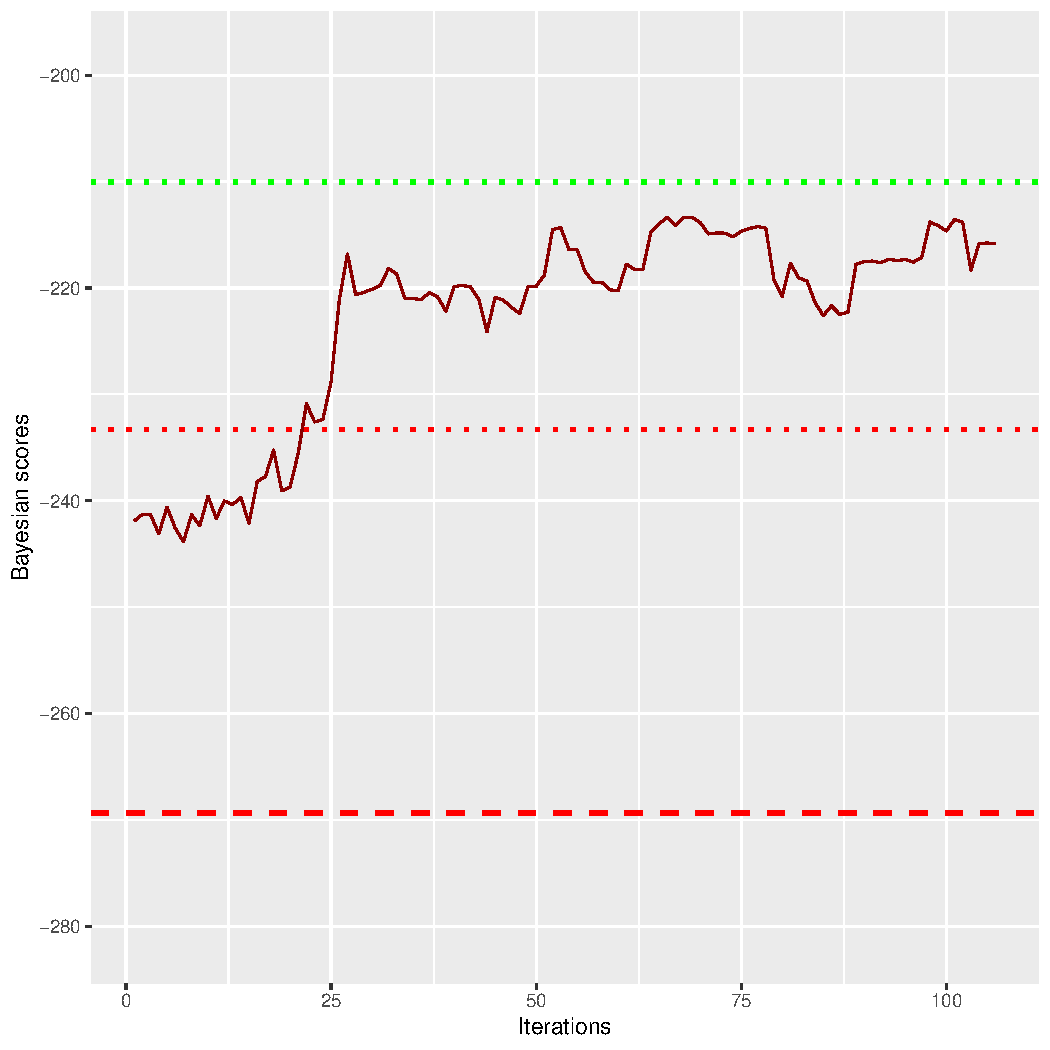
\includegraphics[scale = 0.4]{./figs/asia/v1/20/bayBoundsEvolution-107.pdf} \\
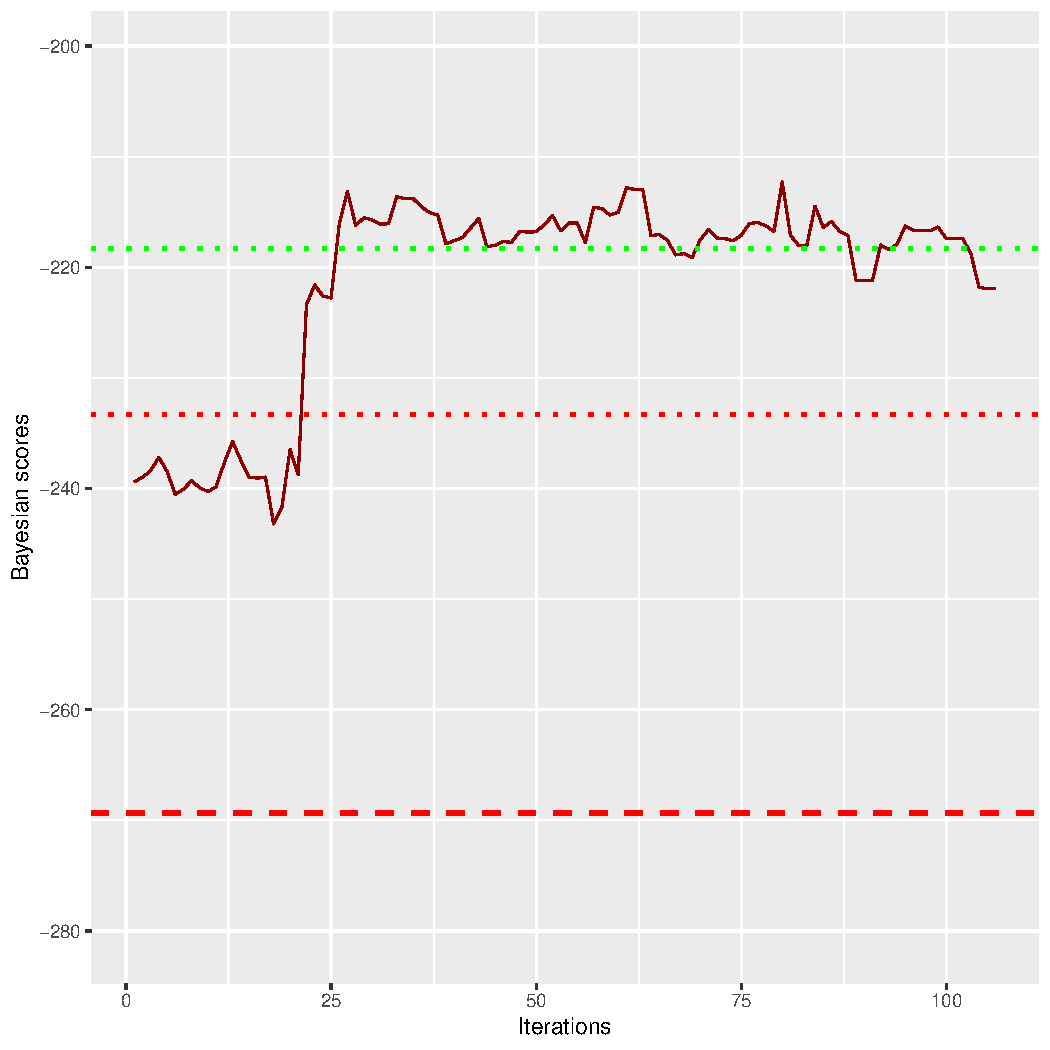
\includegraphics[scale = 0.4]{./figs/asia/v1/30/bayBoundsEvolution-107.pdf} & 
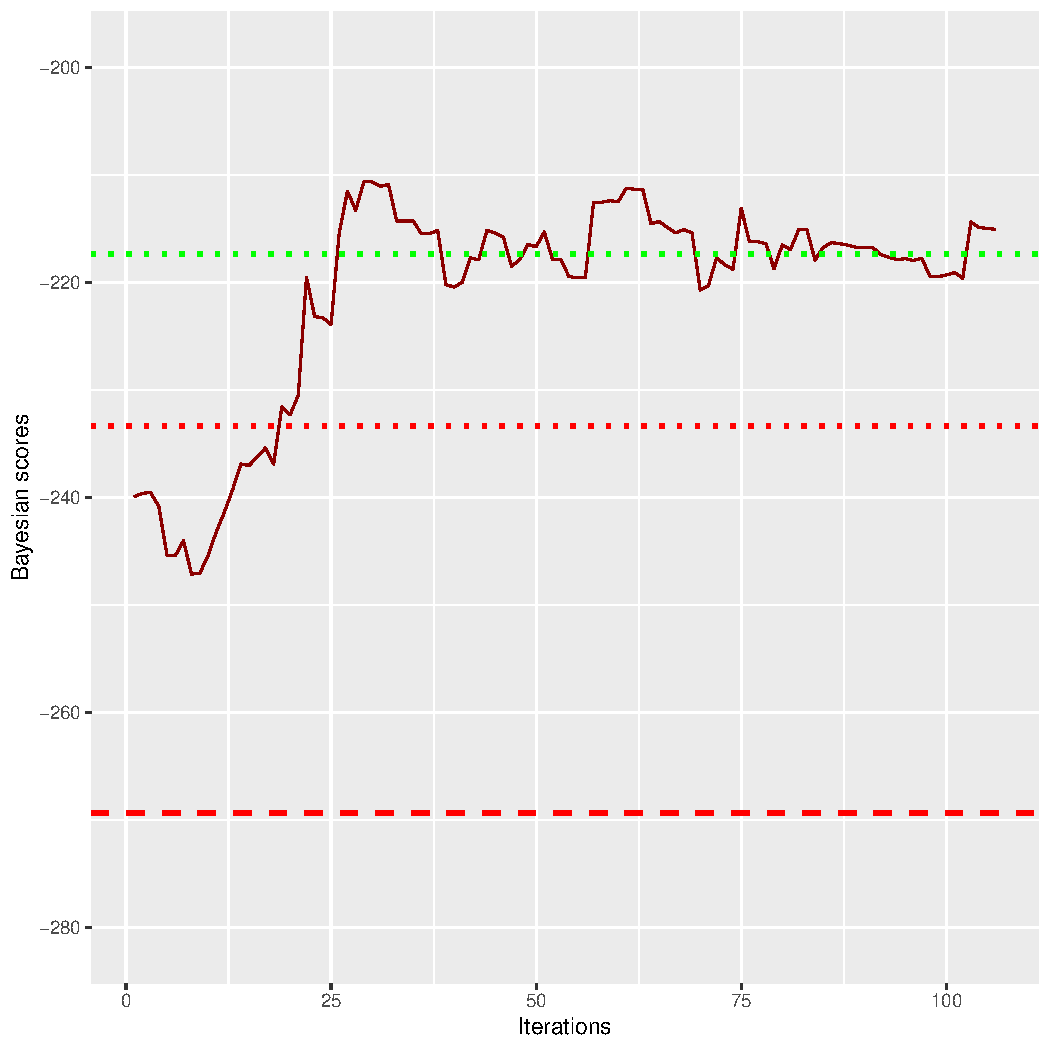
\includegraphics[scale = 0.4]{./figs/asia/v1/40/bayBoundsEvolution-107.pdf} \\
\end{tabular}
\caption{Bayesian score for variant 1 with \textbf{np =  10, 20, 30, 40}}
\end{table}

\clearpage

\subsection{Graphics of evolution for variant 2}

\begin{table}[h!]
\begin{tabular}{cc}
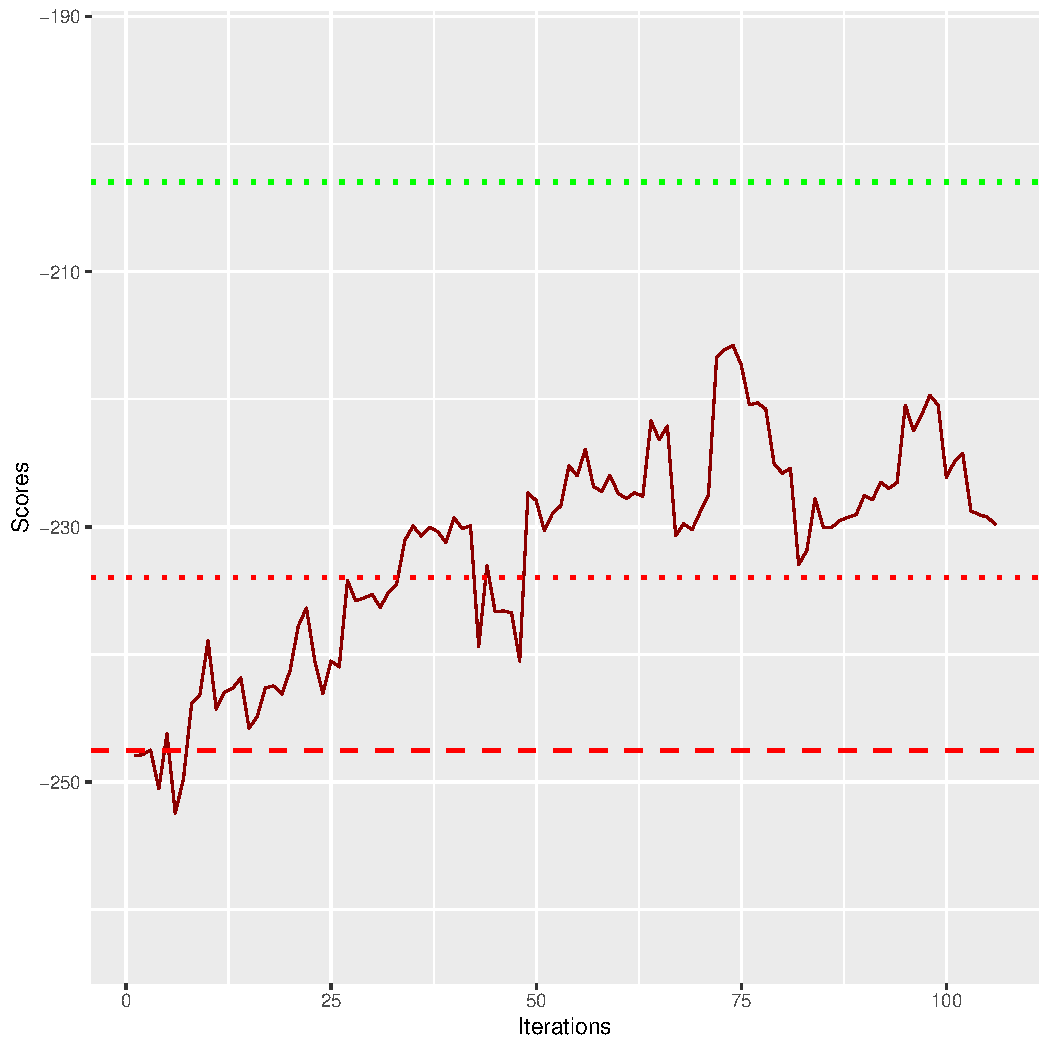
\includegraphics[scale = 0.4]{./figs/asia/v2/10/boundsEvolution-107.pdf} & 
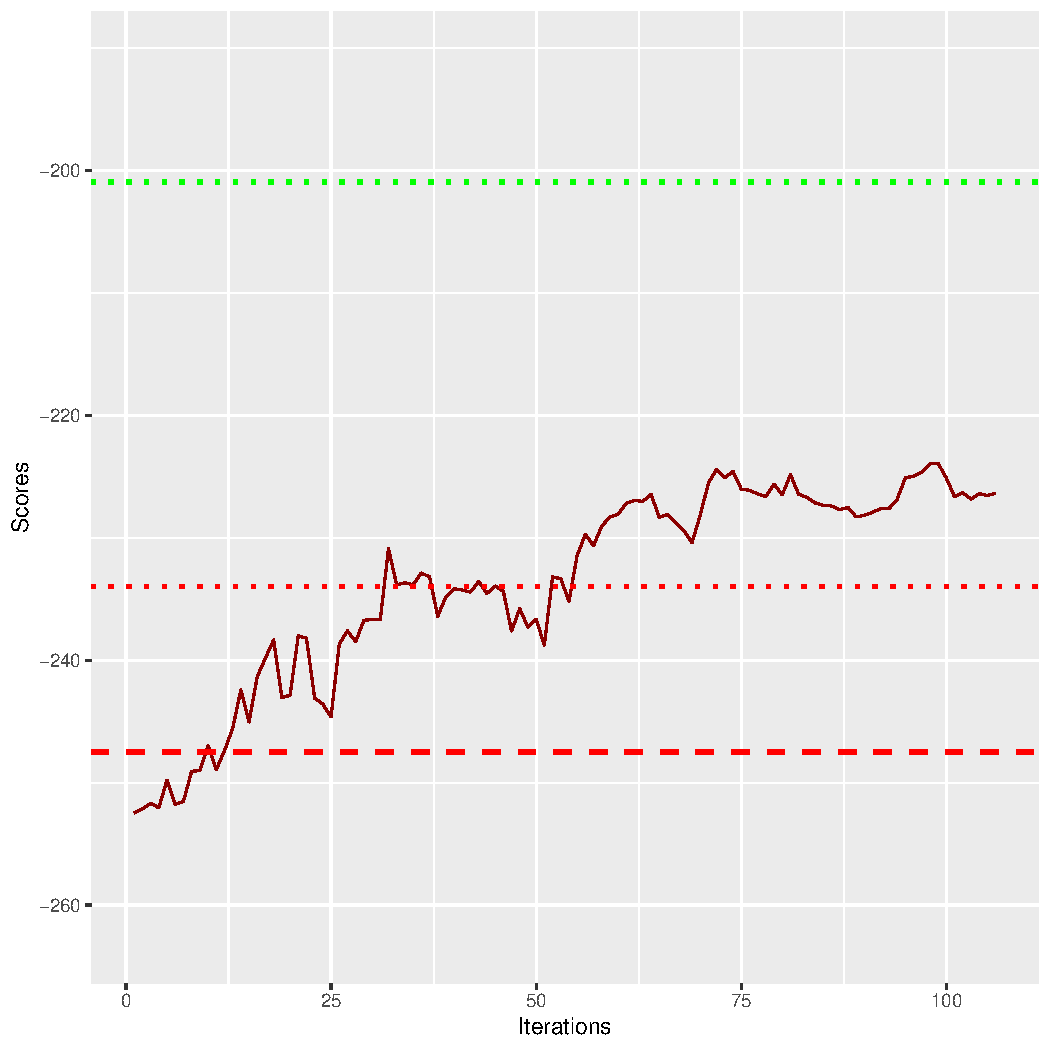
\includegraphics[scale = 0.4]{./figs/asia/v2/20/boundsEvolution-107.pdf} \\
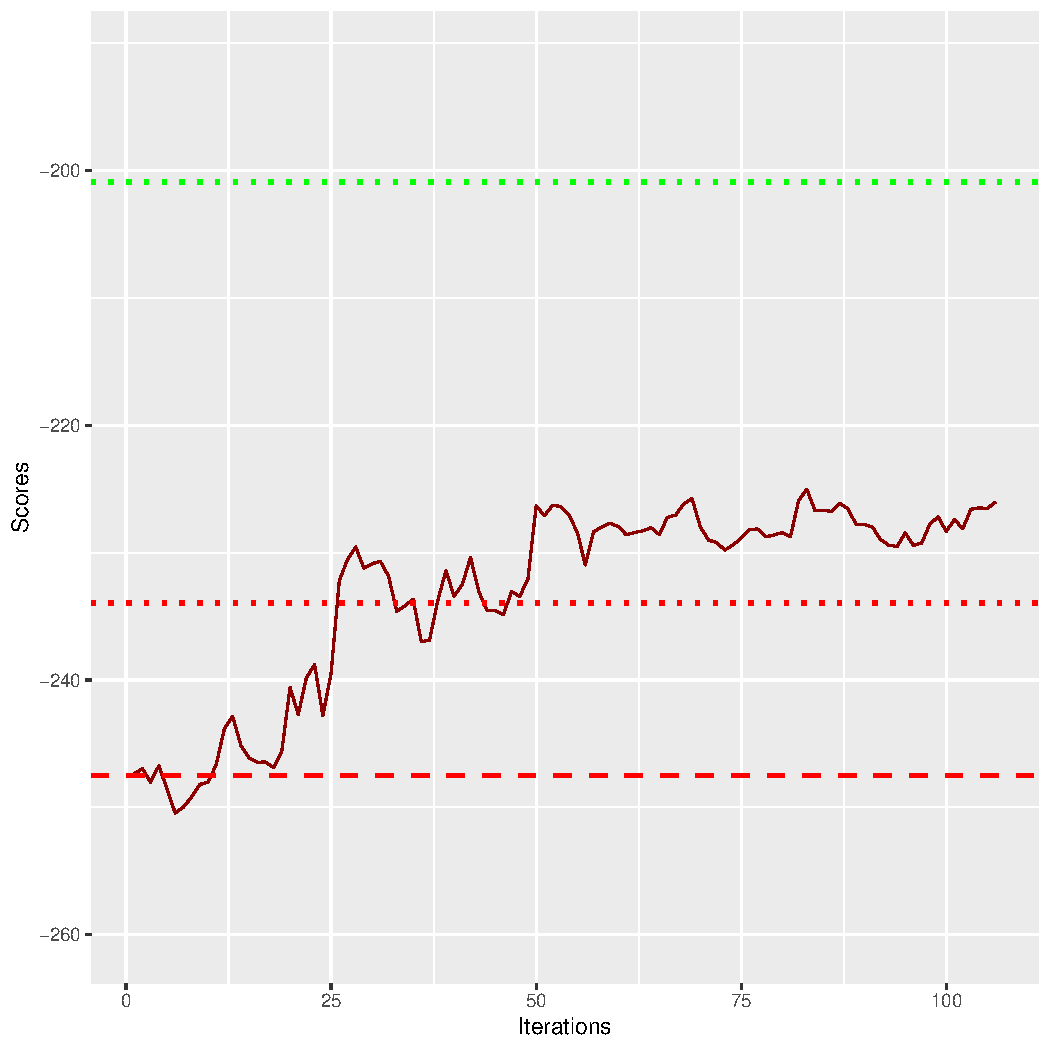
\includegraphics[scale = 0.4]{./figs/asia/v2/30/boundsEvolution-107.pdf} & 
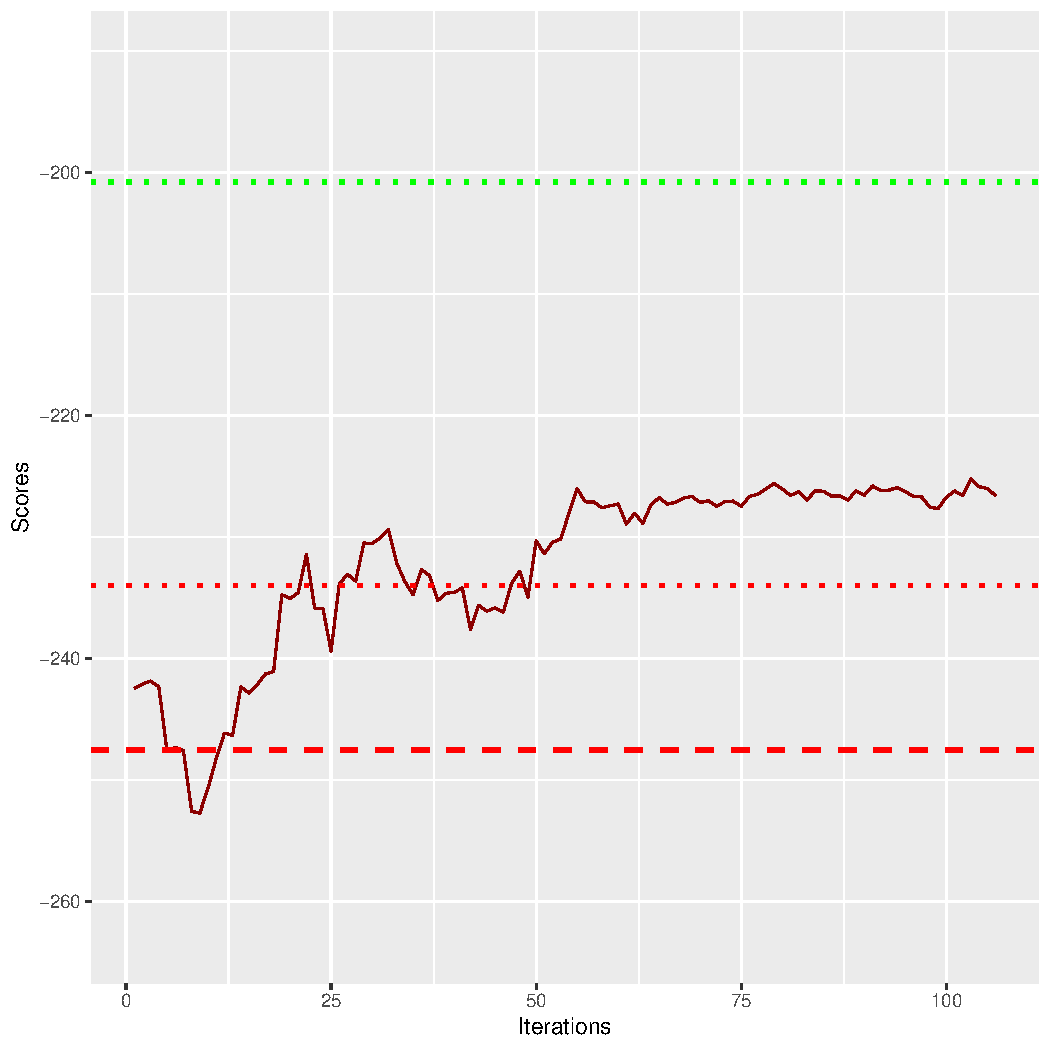
\includegraphics[scale = 0.4]{./figs/asia/v2/40/boundsEvolution-107.pdf} \\
\end{tabular}
\caption{Normal score for variant 2 with \textbf{np =  10, 20, 30, 40}}
\end{table}

\begin{table}[h!]
\begin{tabular}{cc}
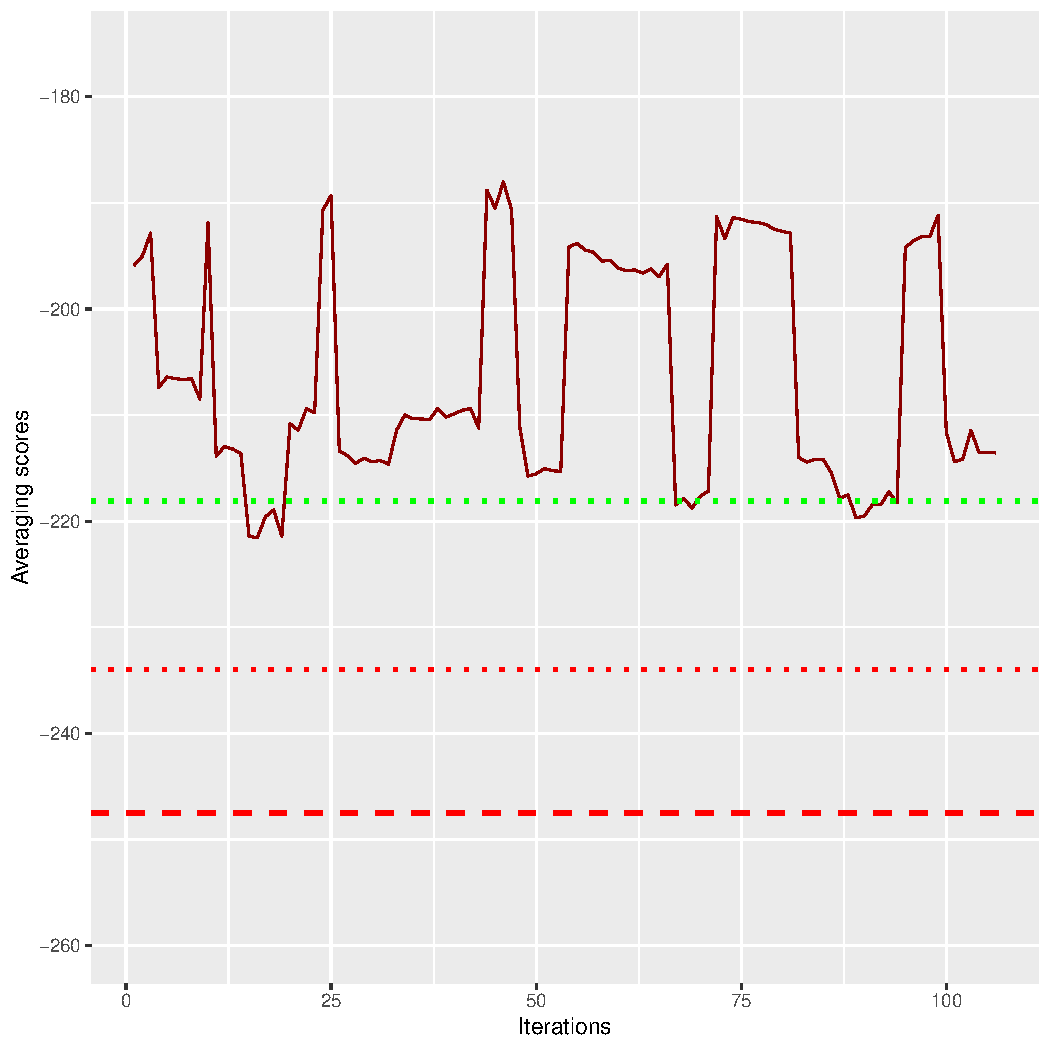
\includegraphics[scale = 0.4]{./figs/asia/v2/10/avgBoundsEvolution-107.pdf} & 
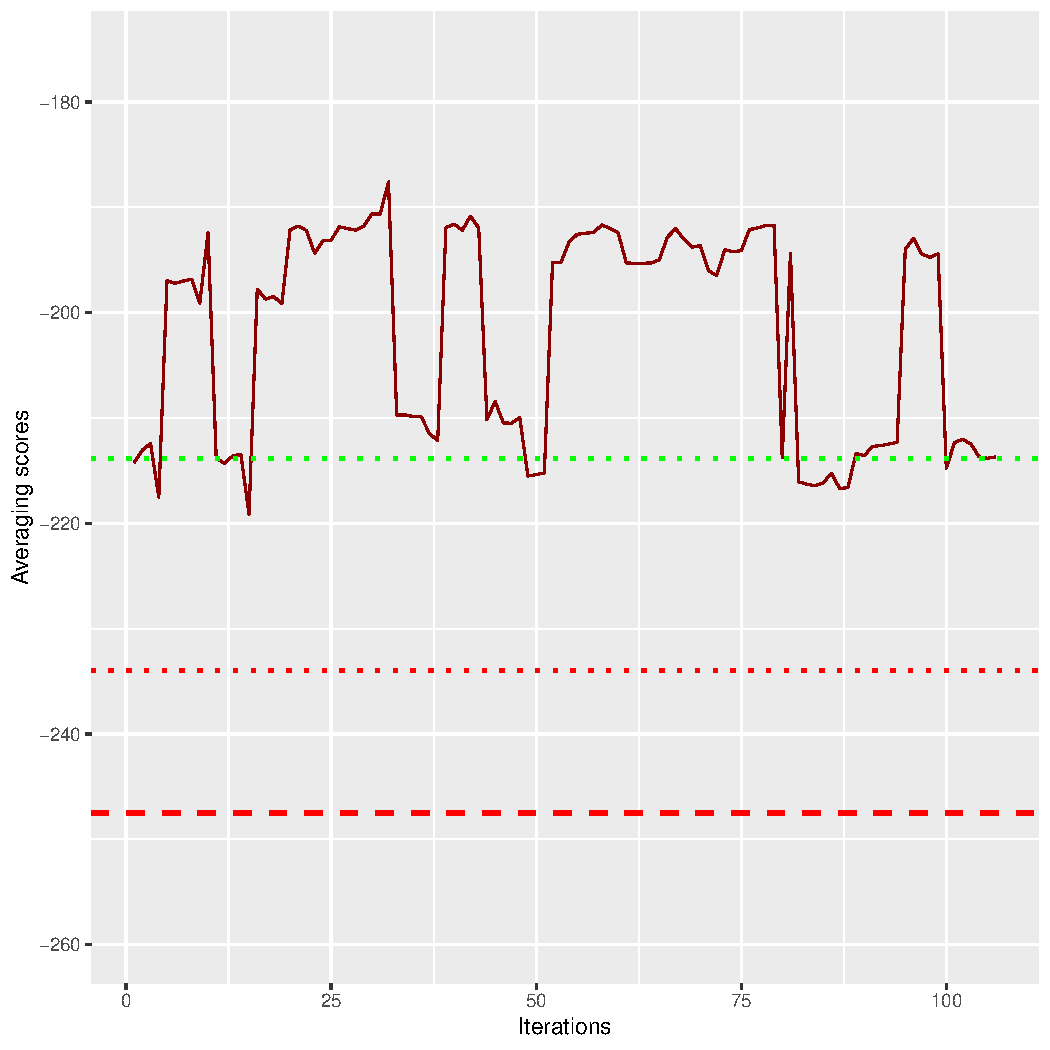
\includegraphics[scale = 0.4]{./figs/asia/v2/20/avgBoundsEvolution-107.pdf} \\
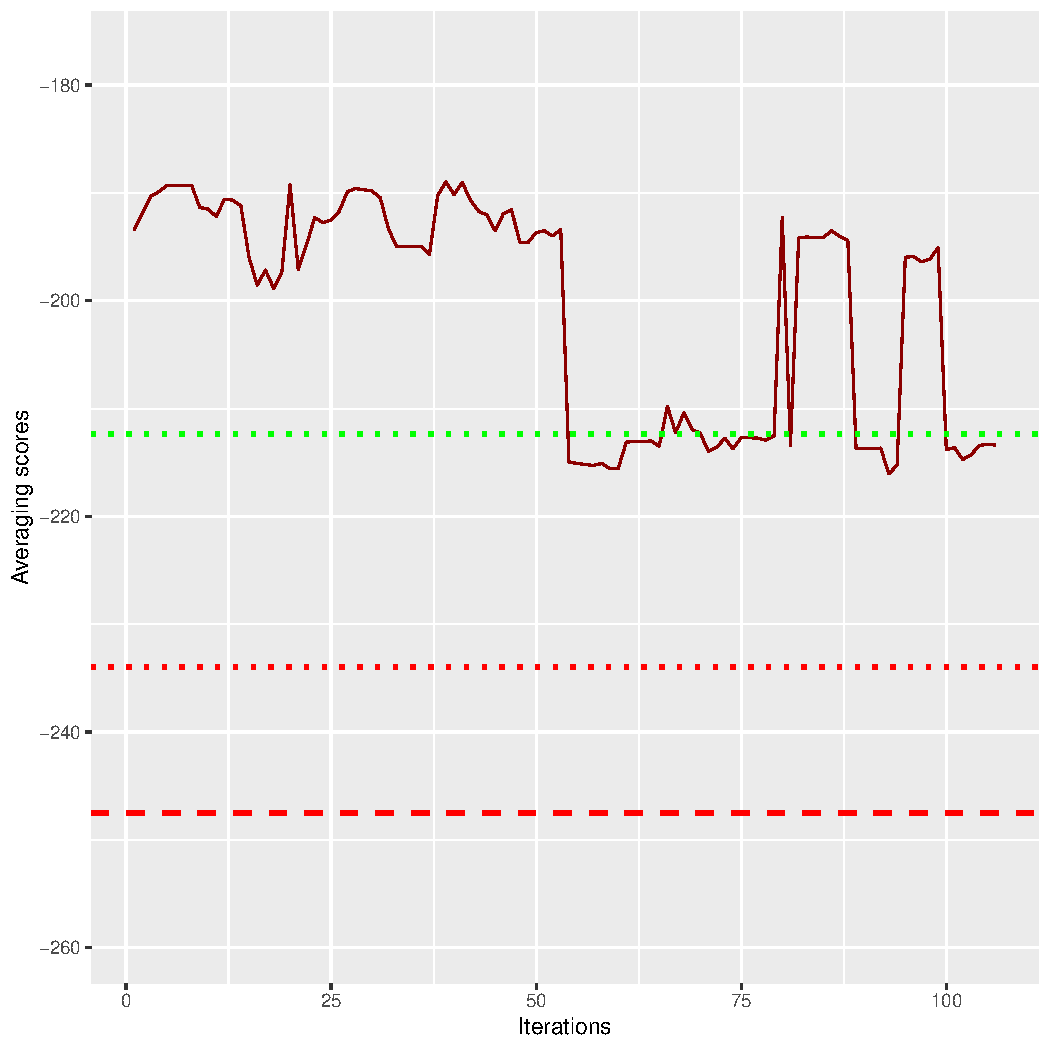
\includegraphics[scale = 0.4]{./figs/asia/v2/30/avgBoundsEvolution-107.pdf} & 
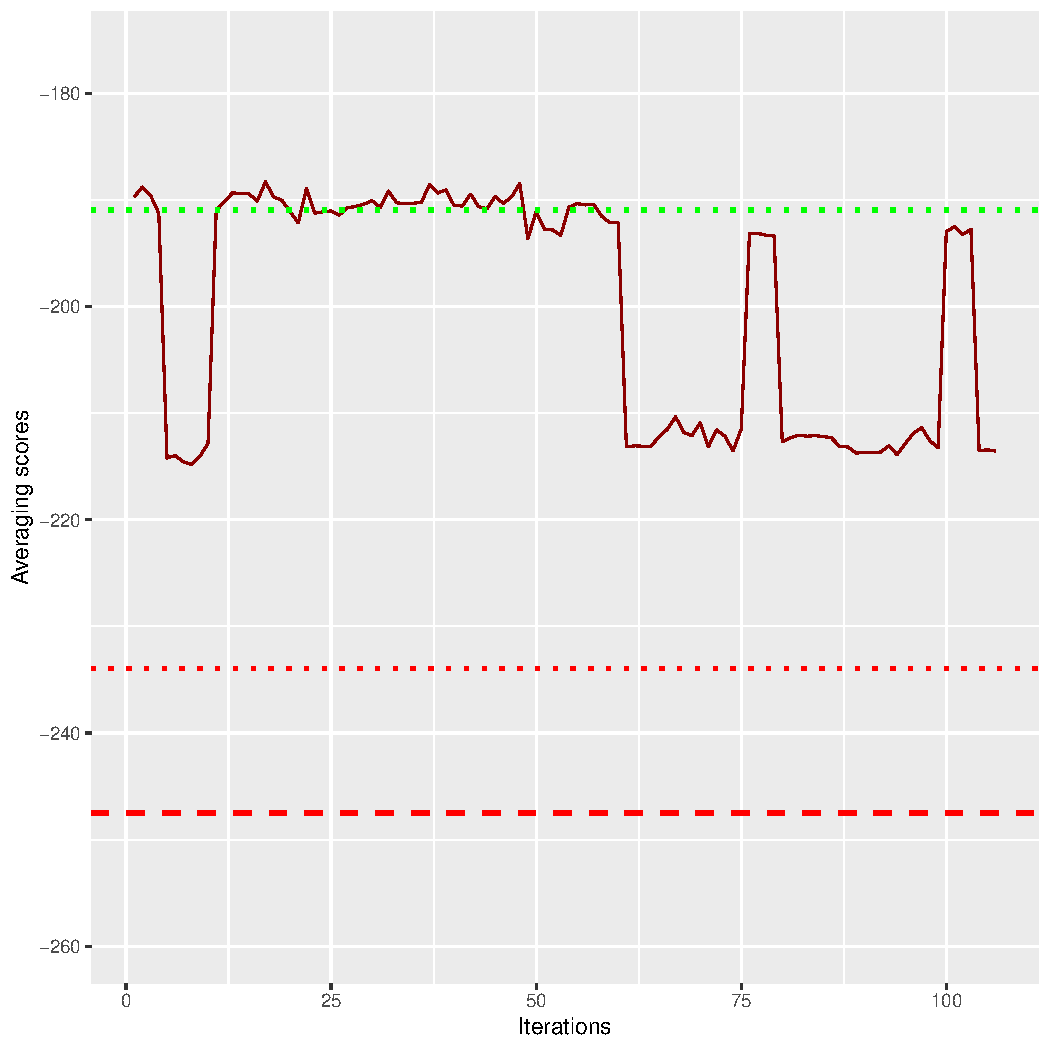
\includegraphics[scale = 0.4]{./figs/asia/v2/40/avgBoundsEvolution-107.pdf} \\
\end{tabular}
\caption{Averaging score for variant 2 with \textbf{np =  10, 20, 30, 40}}
\end{table}

\begin{table}[h!]
\begin{tabular}{cc}
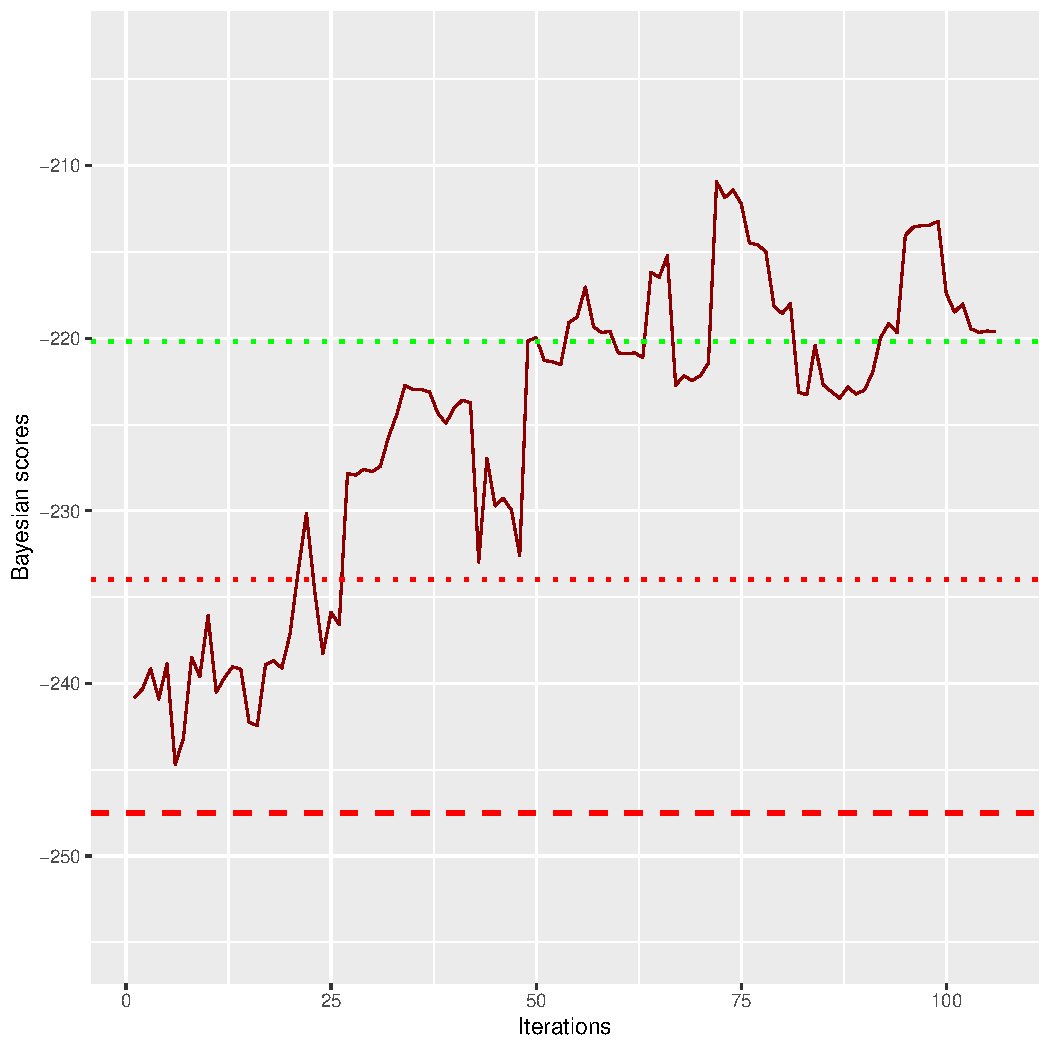
\includegraphics[scale = 0.4]{./figs/asia/v2/10/bayBoundsEvolution-107.pdf} & 
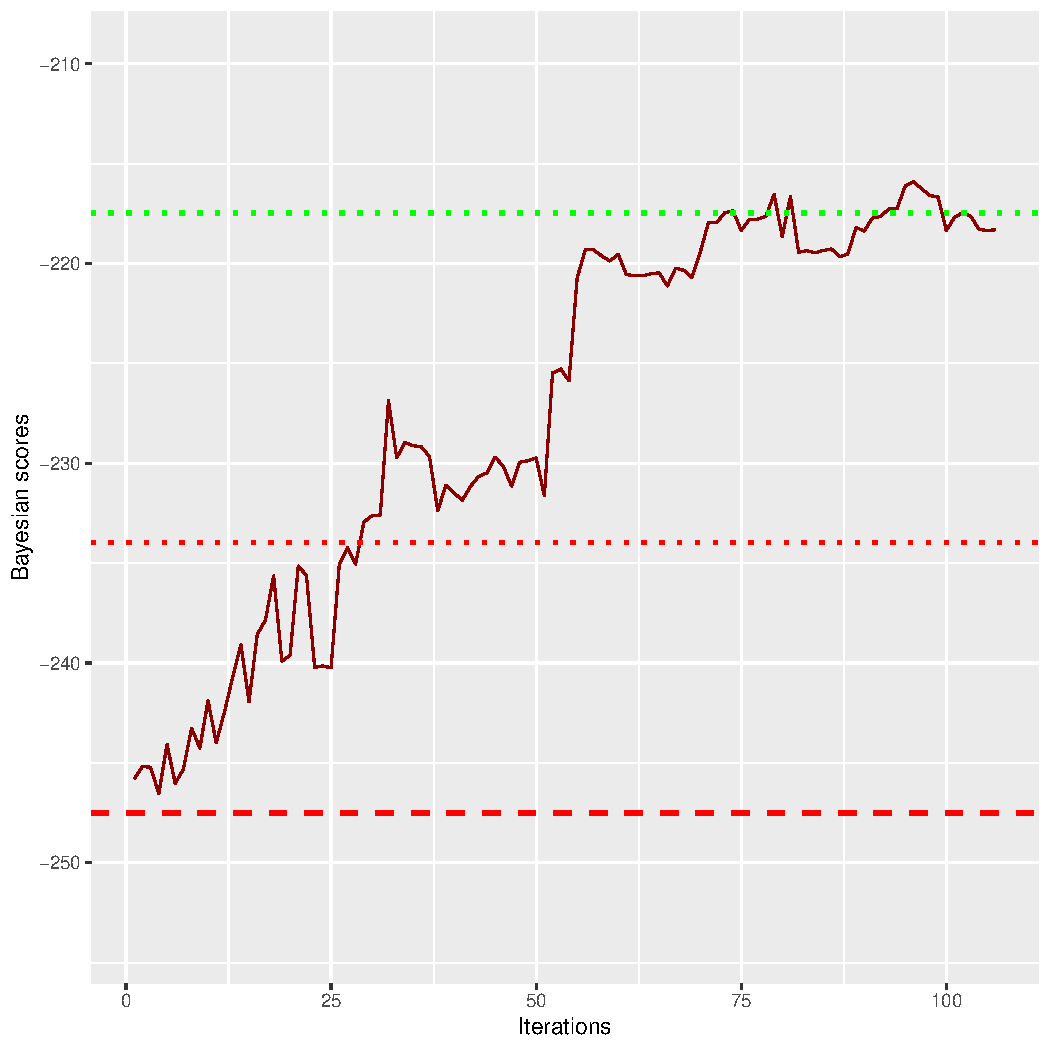
\includegraphics[scale = 0.4]{./figs/asia/v2/20/bayBoundsEvolution-107.pdf} \\
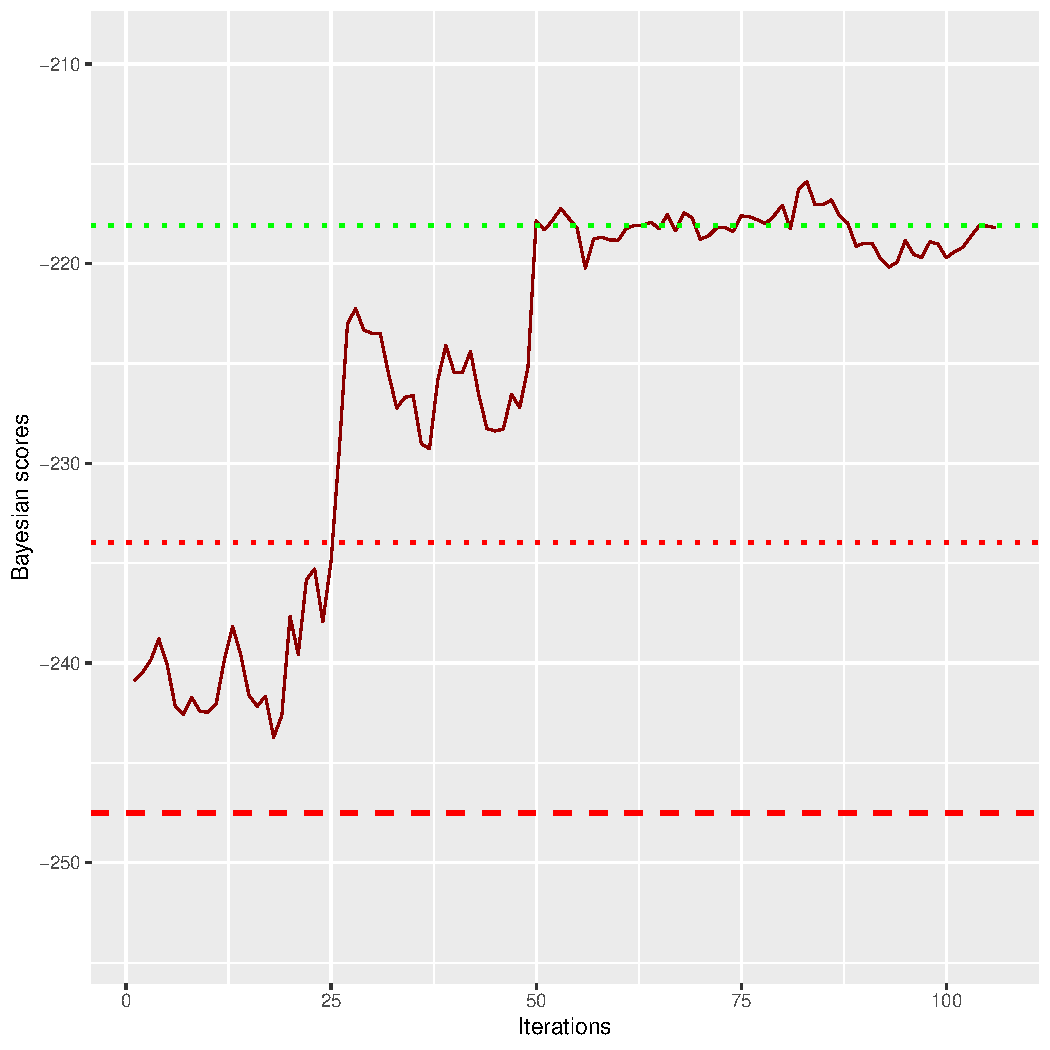
\includegraphics[scale = 0.4]{./figs/asia/v2/30/bayBoundsEvolution-107.pdf} & 
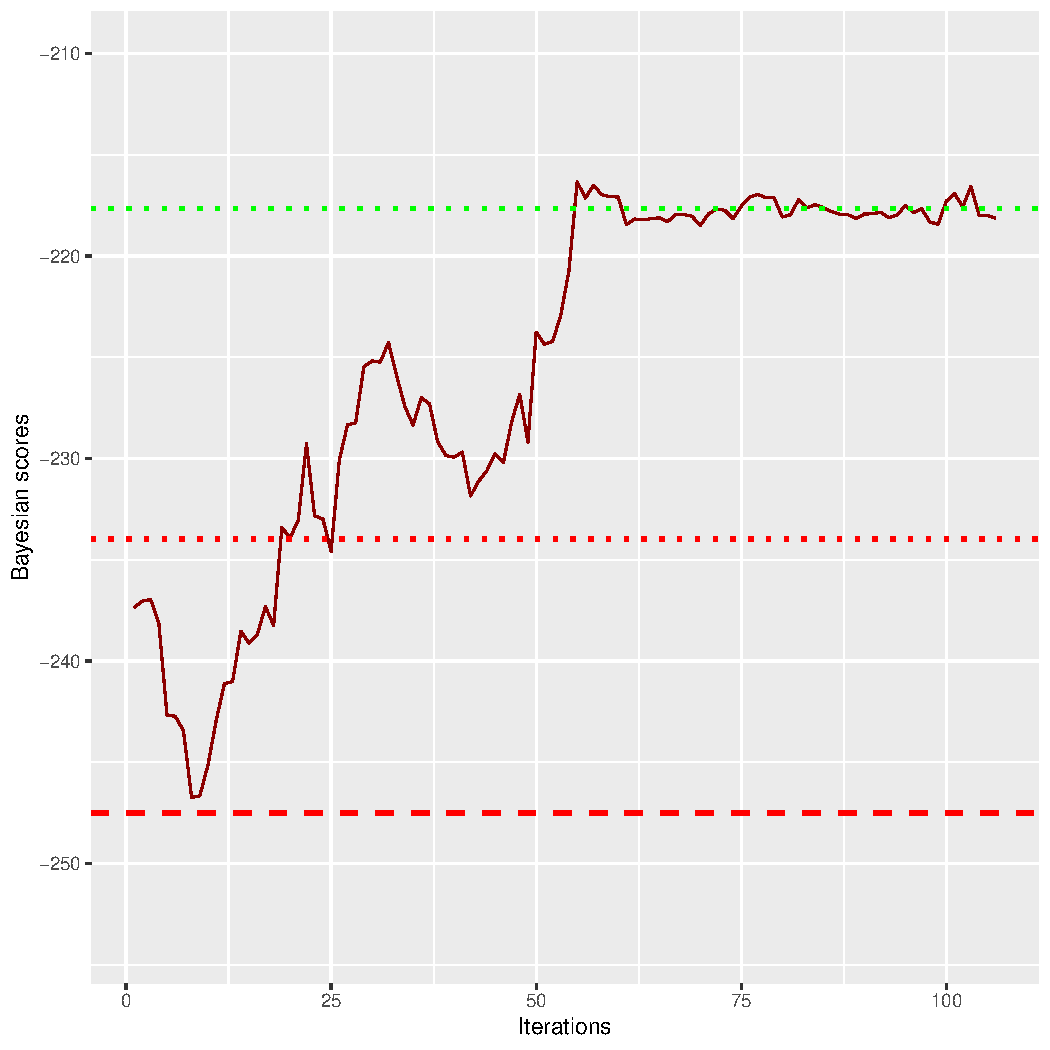
\includegraphics[scale = 0.4]{./figs/asia/v2/40/bayBoundsEvolution-107.pdf} \\
\end{tabular}
\caption{Bayesian score for variant 2 with \textbf{np =  10, 20, 30, 40}}
\end{table}

\clearpage

\subsection{Graphics of evolution for variant 3}

\begin{table}[h!]
\begin{tabular}{cc}
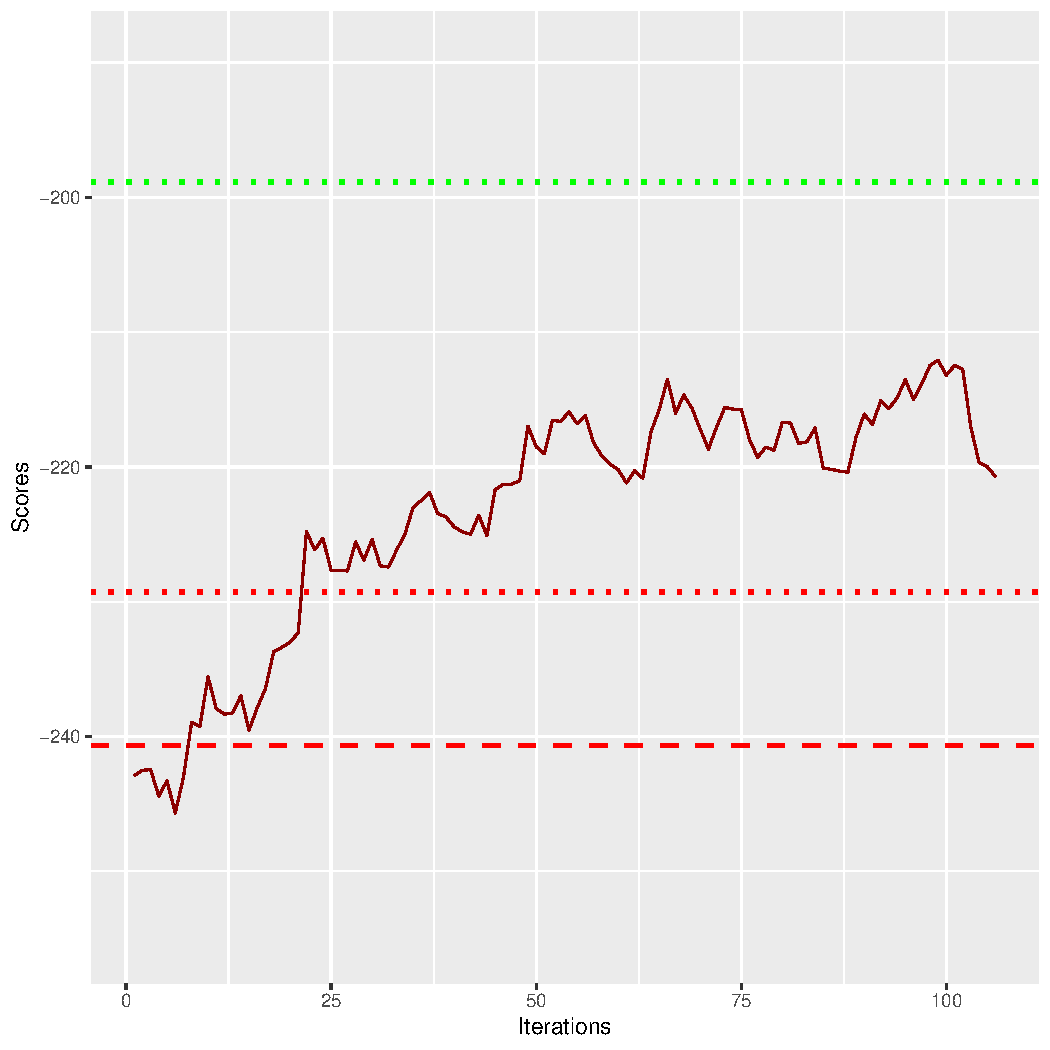
\includegraphics[scale = 0.4]{./figs/asia/v3/10/boundsEvolution-107.pdf} & 
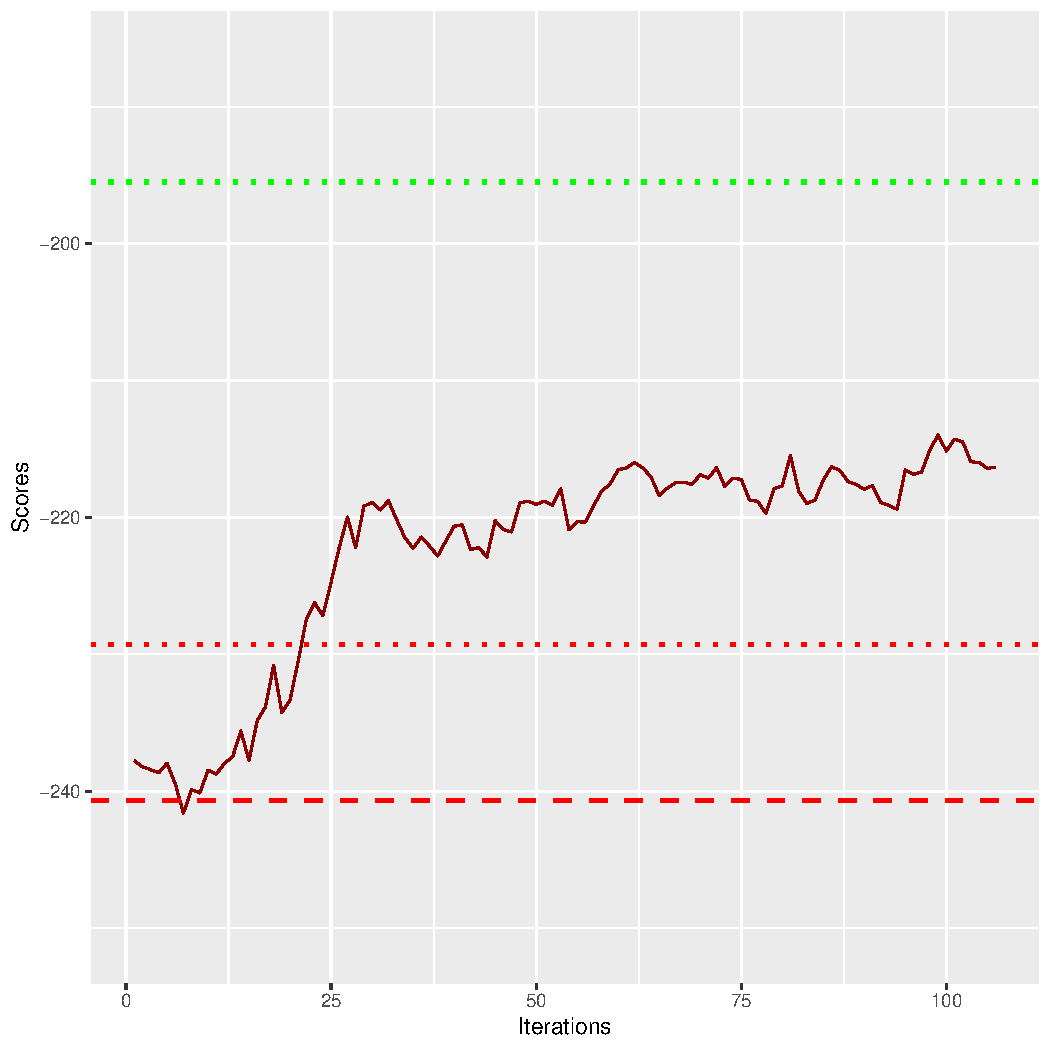
\includegraphics[scale = 0.4]{./figs/asia/v3/20/boundsEvolution-107.pdf} \\
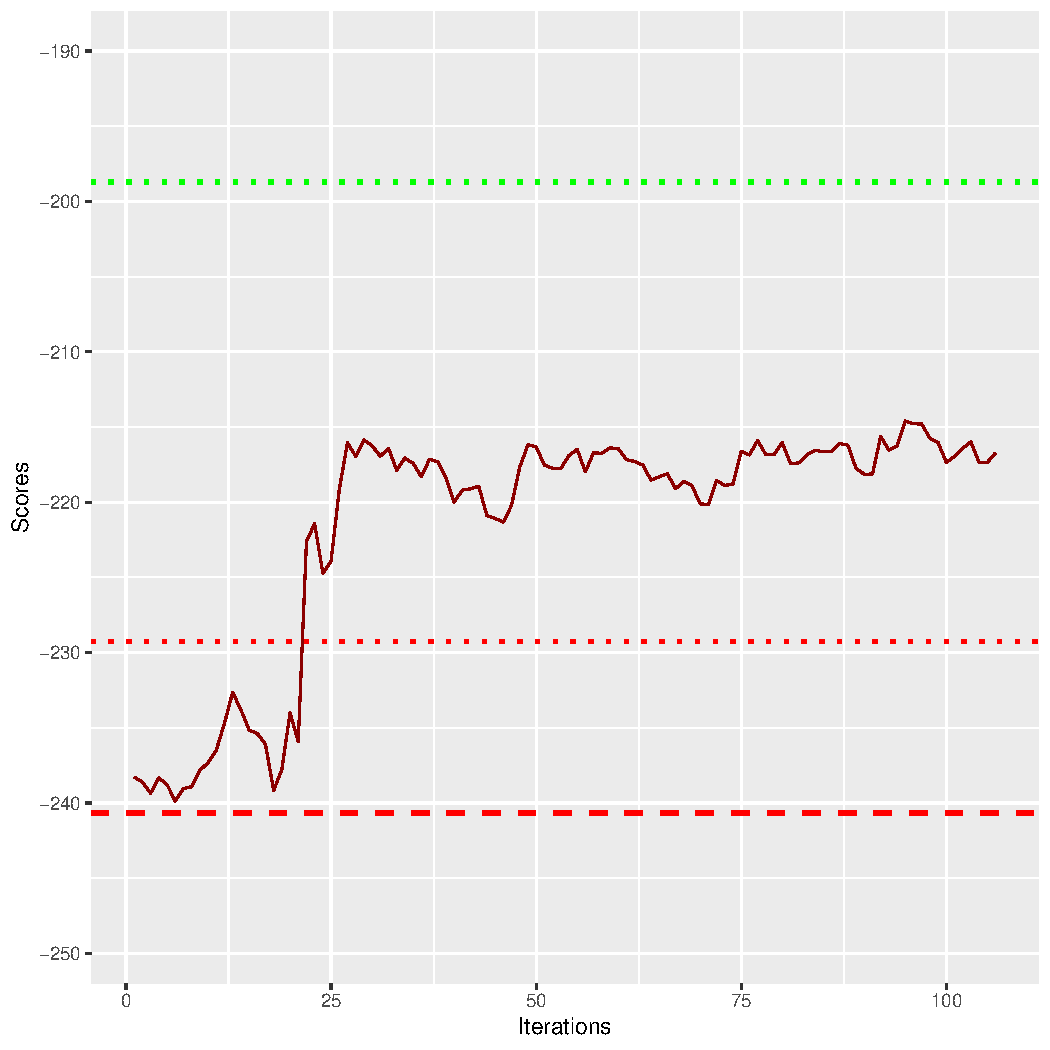
\includegraphics[scale = 0.4]{./figs/asia/v3/30/boundsEvolution-107.pdf} & 
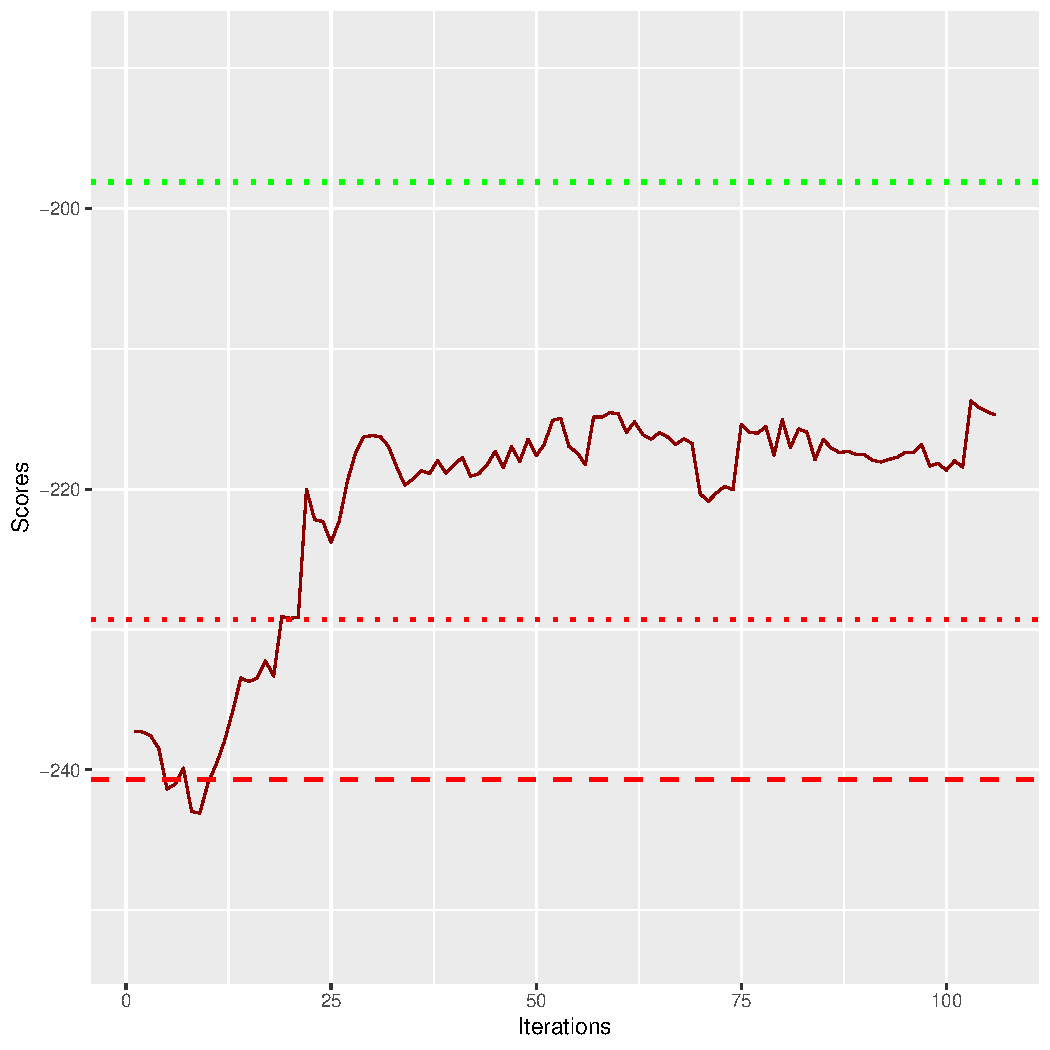
\includegraphics[scale = 0.4]{./figs/asia/v3/40/boundsEvolution-107.pdf} \\
\end{tabular}
\caption{Normal score for variant 3 with \textbf{np =  10, 20, 30, 40}}
\end{table}

\begin{table}[h!]
\begin{tabular}{cc}
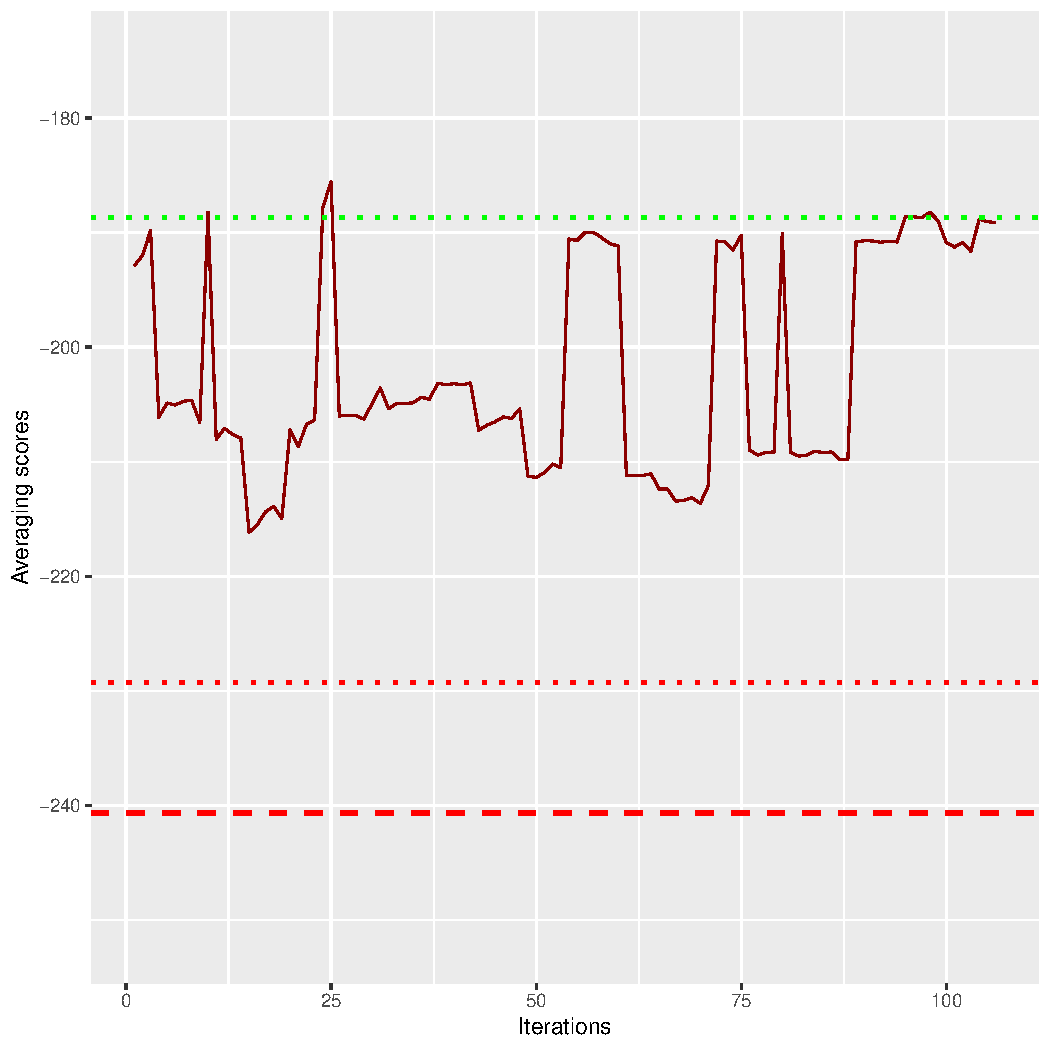
\includegraphics[scale = 0.4]{./figs/asia/v3/10/avgBoundsEvolution-107.pdf} & 
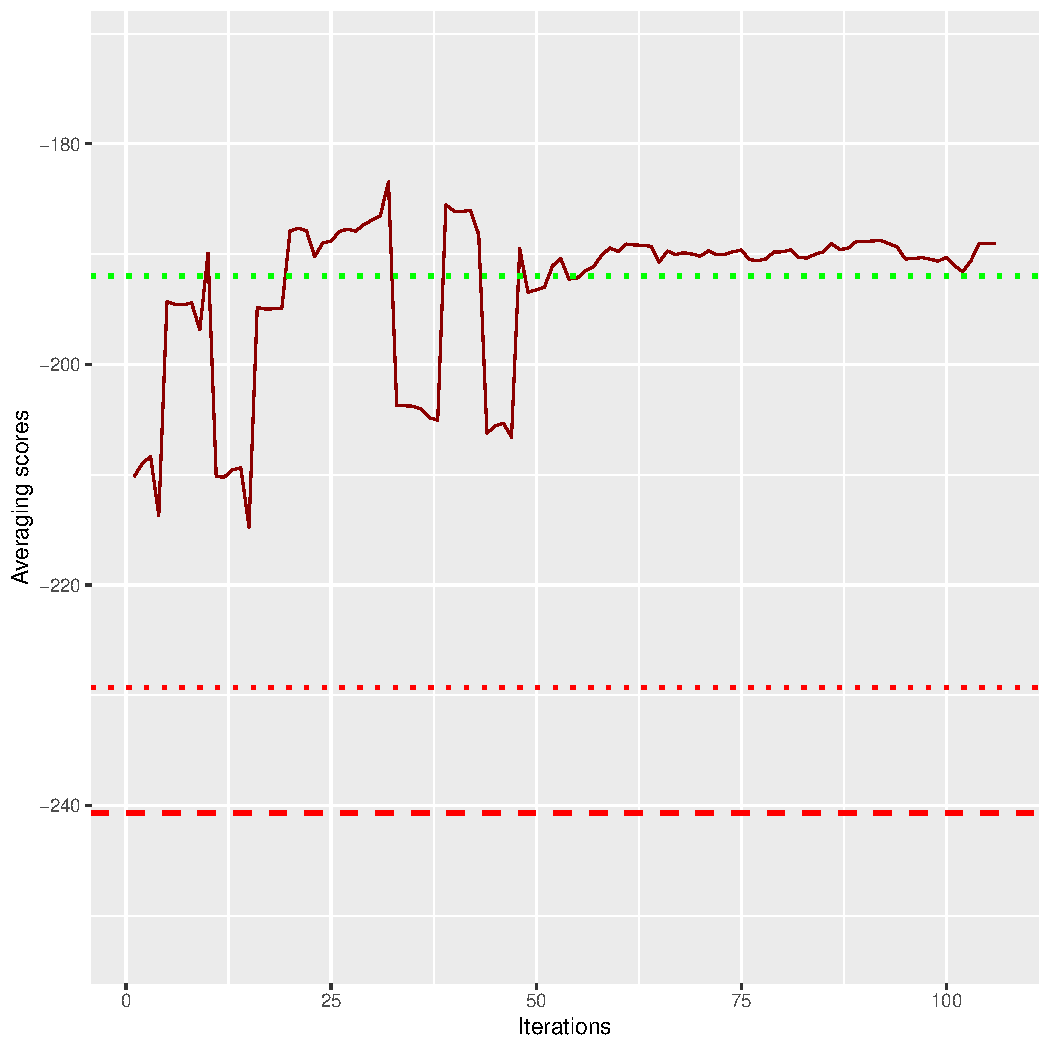
\includegraphics[scale = 0.4]{./figs/asia/v3/20/avgBoundsEvolution-107.pdf} \\
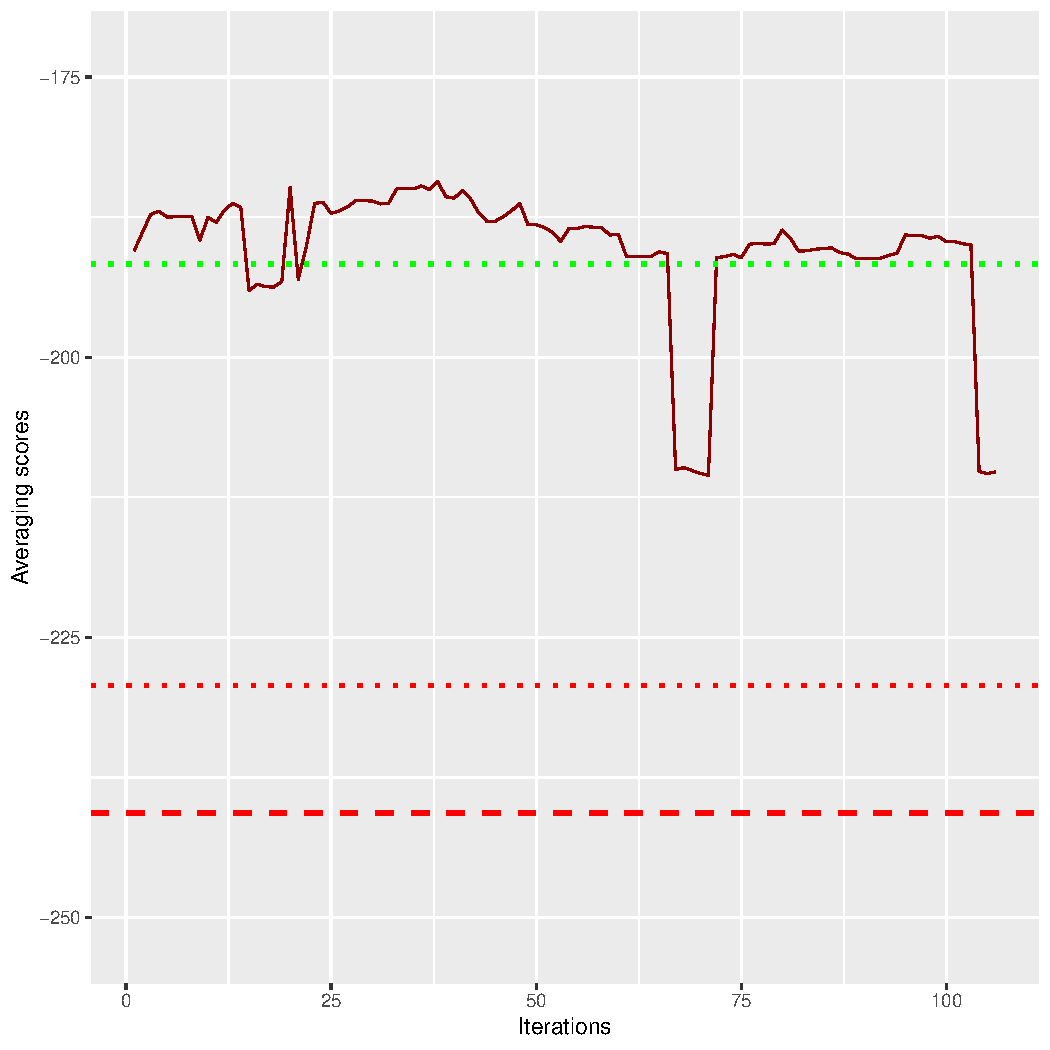
\includegraphics[scale = 0.4]{./figs/asia/v3/30/avgBoundsEvolution-107.pdf} & 
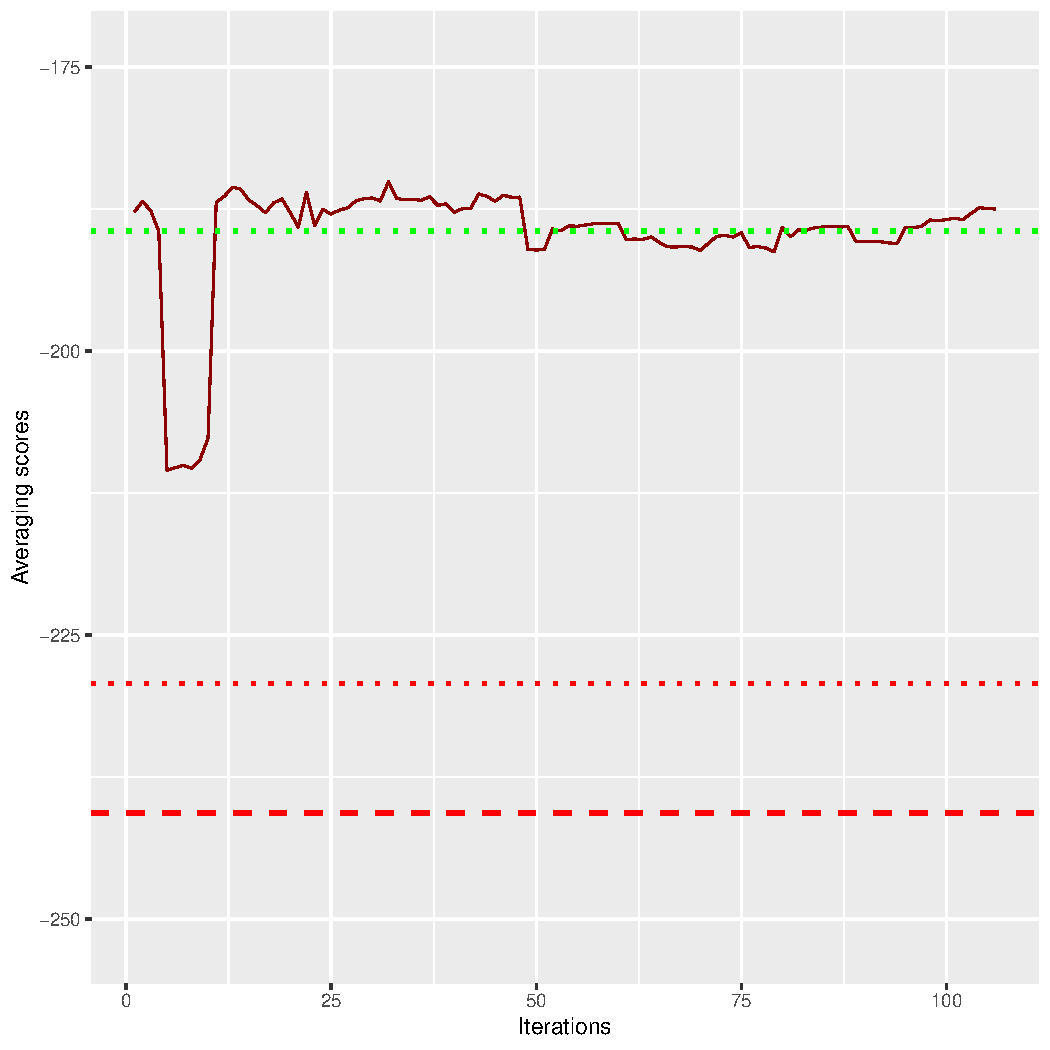
\includegraphics[scale = 0.4]{./figs/asia/v3/40/avgBoundsEvolution-107.pdf} \\
\end{tabular}
\caption{Averaging score for variant 3 with \textbf{np =  10, 20, 30, 40}}
\end{table}

\begin{table}[h!]
\begin{tabular}{cc}
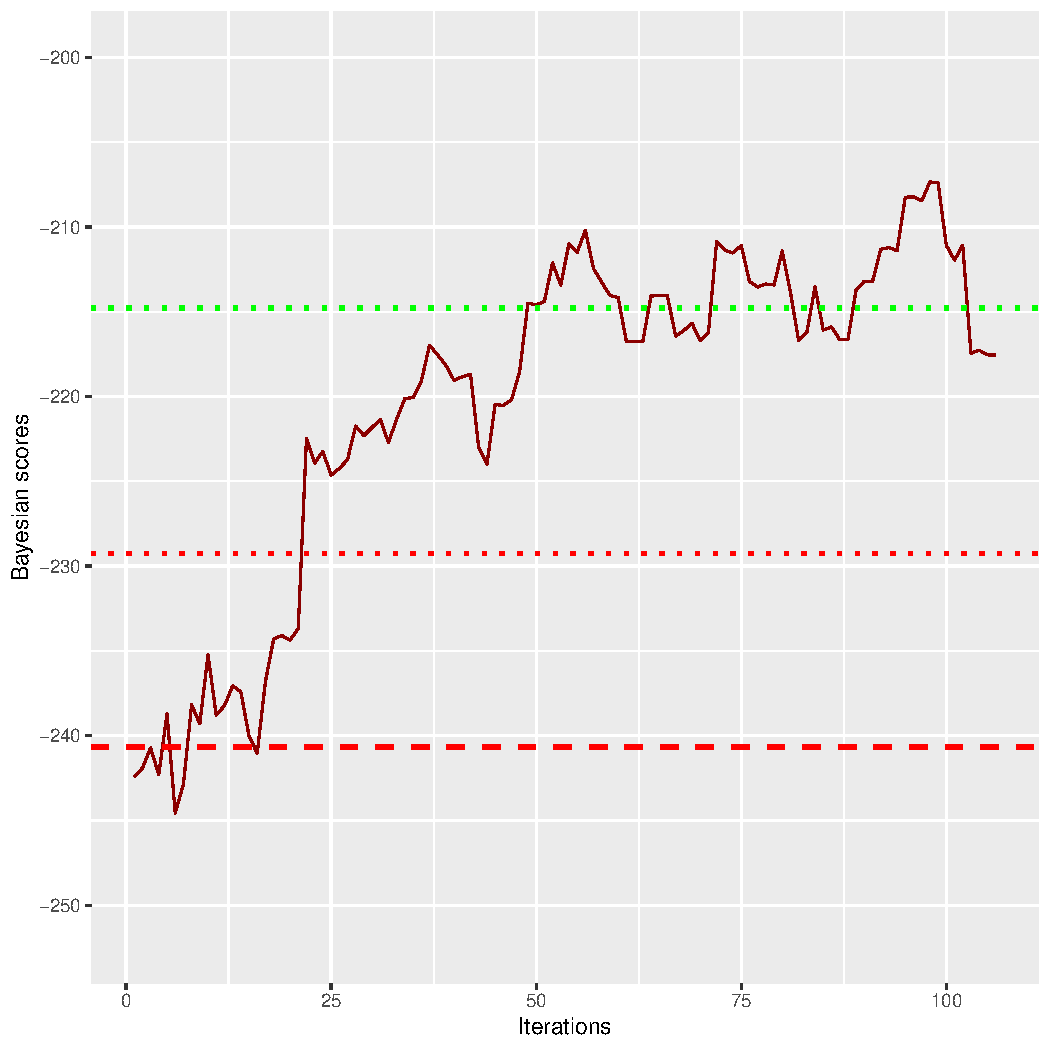
\includegraphics[scale = 0.4]{./figs/asia/v3/10/bayBoundsEvolution-107.pdf} & 
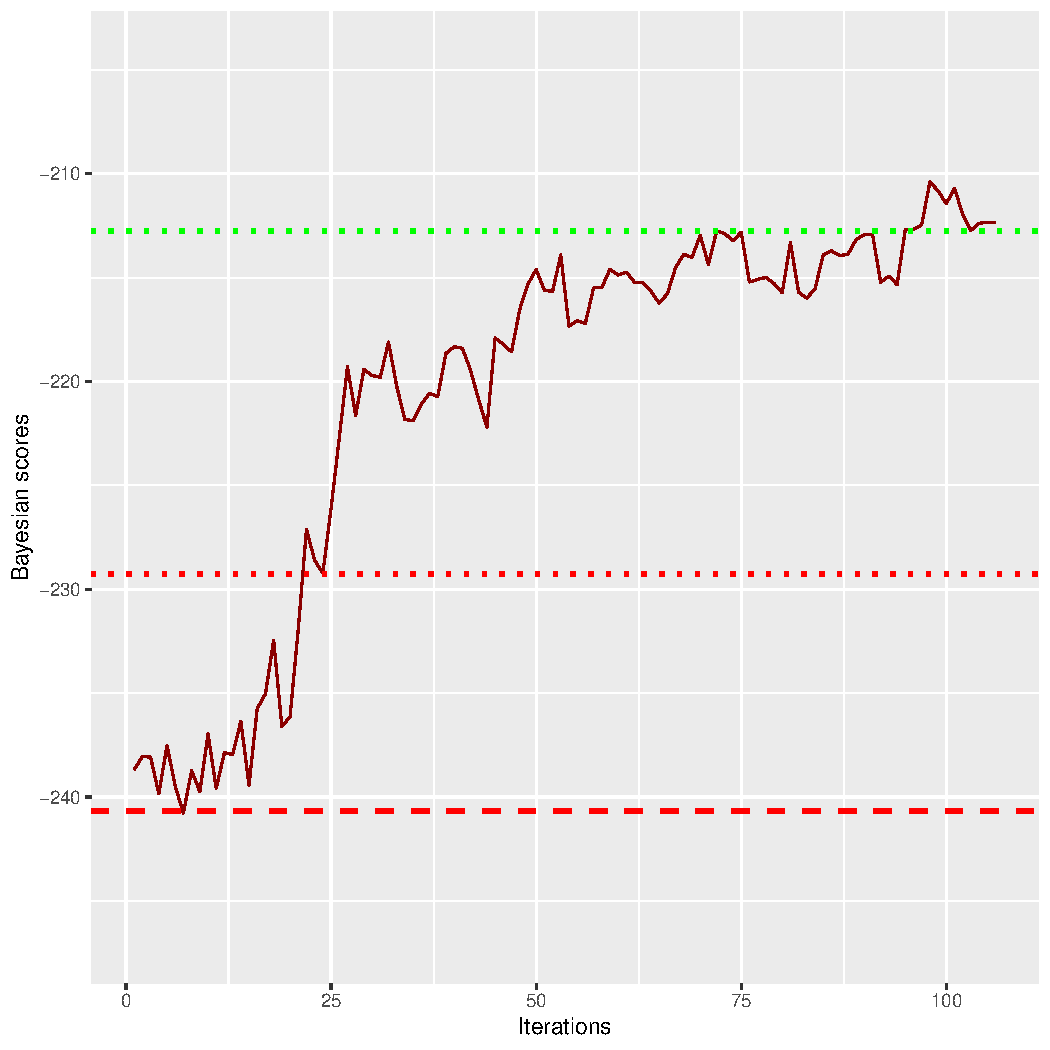
\includegraphics[scale = 0.4]{./figs/asia/v3/20/bayBoundsEvolution-107.pdf} \\
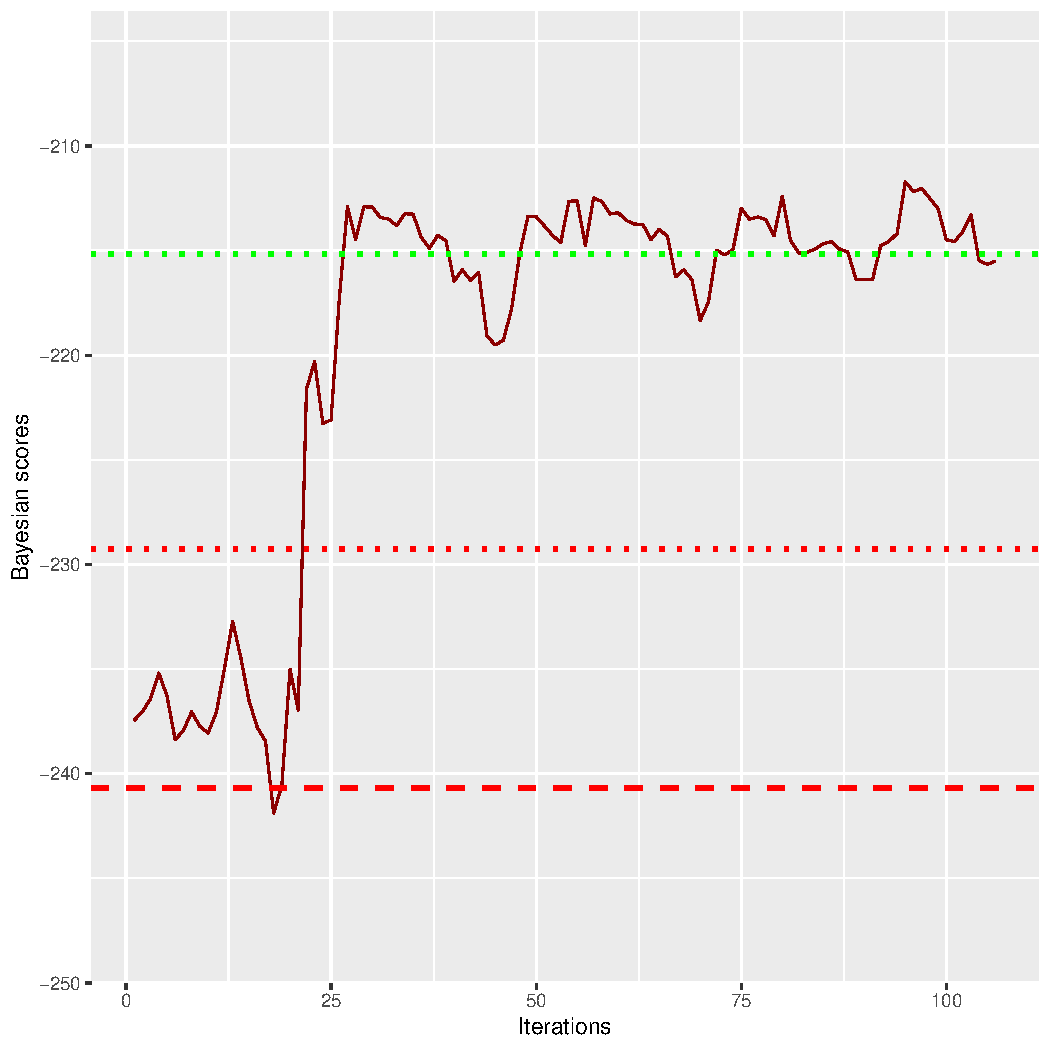
\includegraphics[scale = 0.4]{./figs/asia/v3/30/bayBoundsEvolution-107.pdf} & 
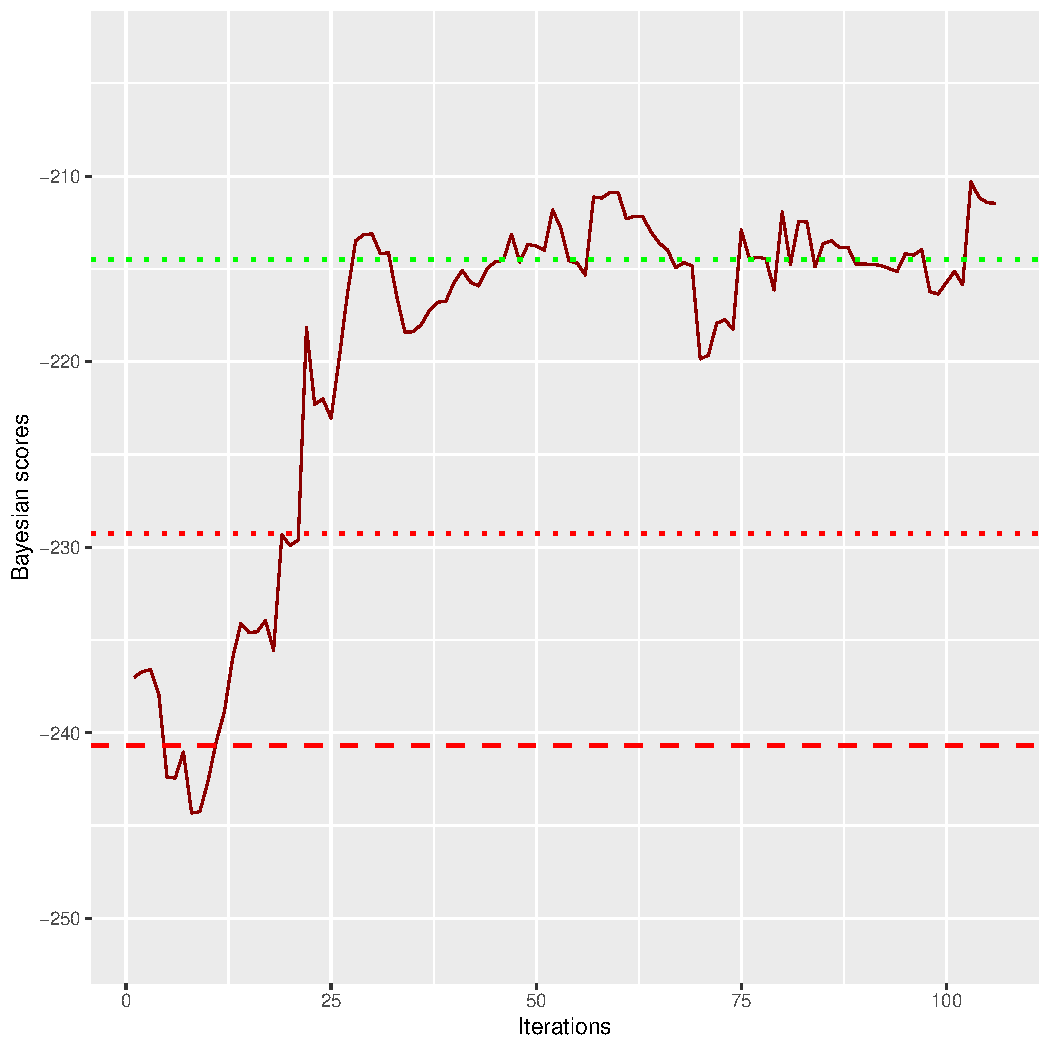
\includegraphics[scale = 0.4]{./figs/asia/v3/40/bayBoundsEvolution-107.pdf} \\
\end{tabular}
\caption{Bayesian score for variant 3 with \textbf{np =  10, 20, 30, 40}}
\end{table}

\clearpage

\subsection{Graphics of evolution for variant 4}

\begin{table}[h!]
\begin{tabular}{cc}
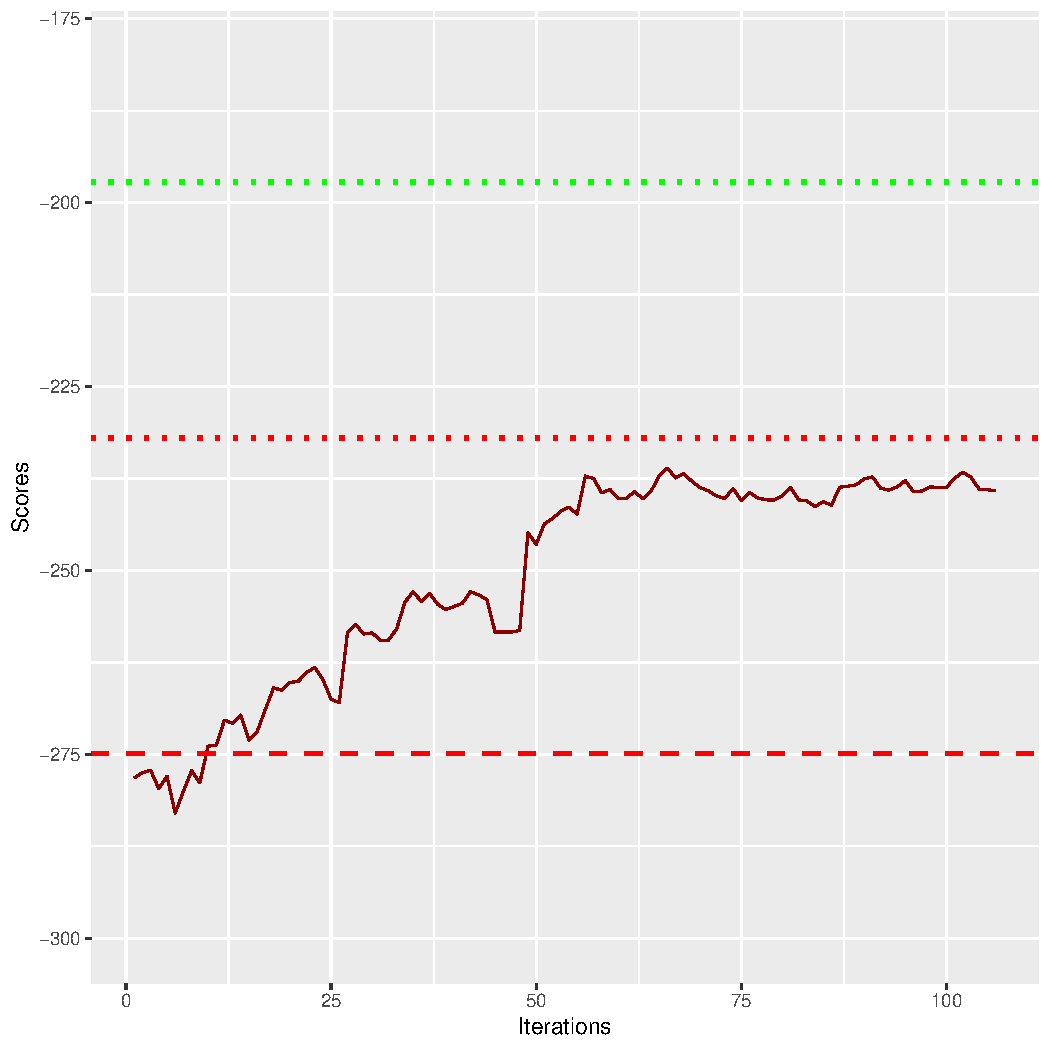
\includegraphics[scale = 0.4]{./figs/asia/v4/10/boundsEvolution-107.pdf} & 
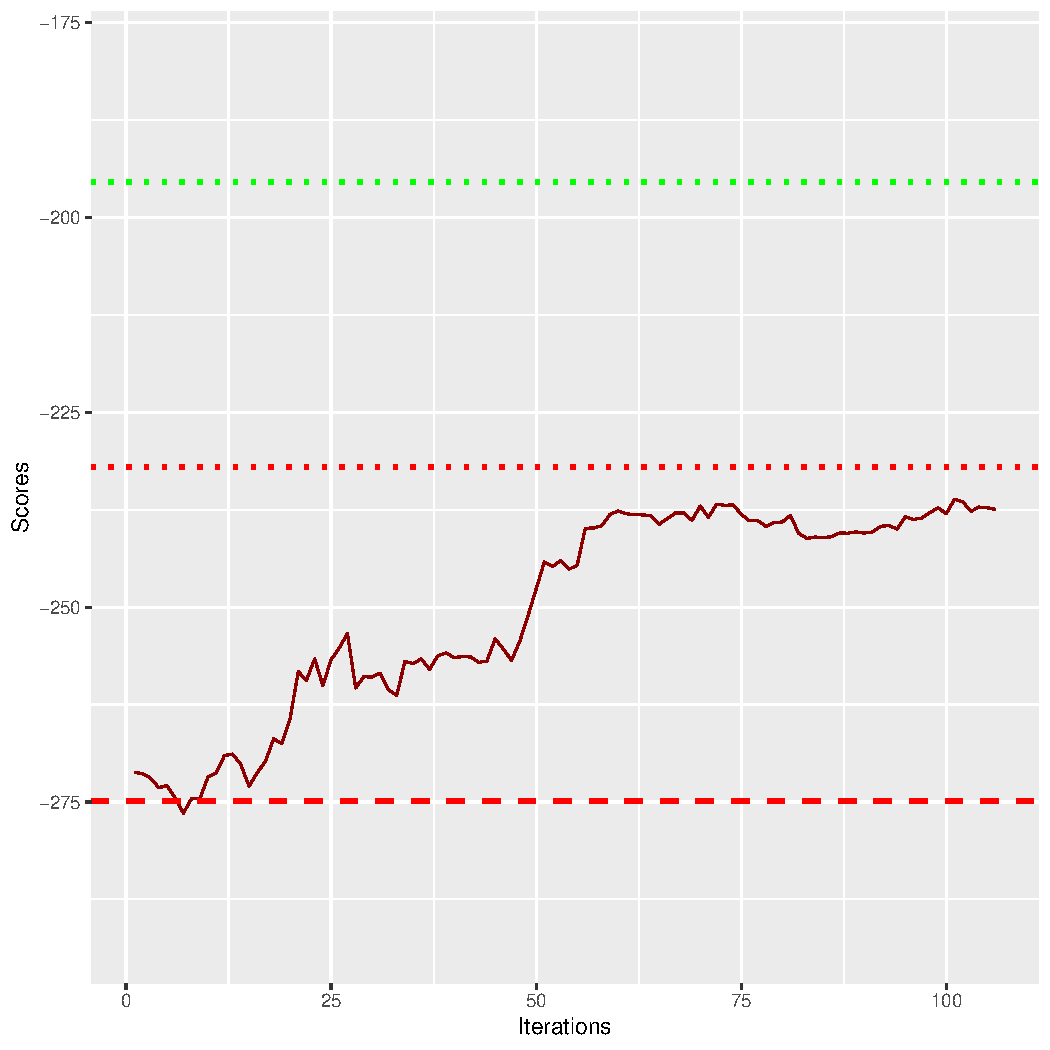
\includegraphics[scale = 0.4]{./figs/asia/v4/20/boundsEvolution-107.pdf} \\
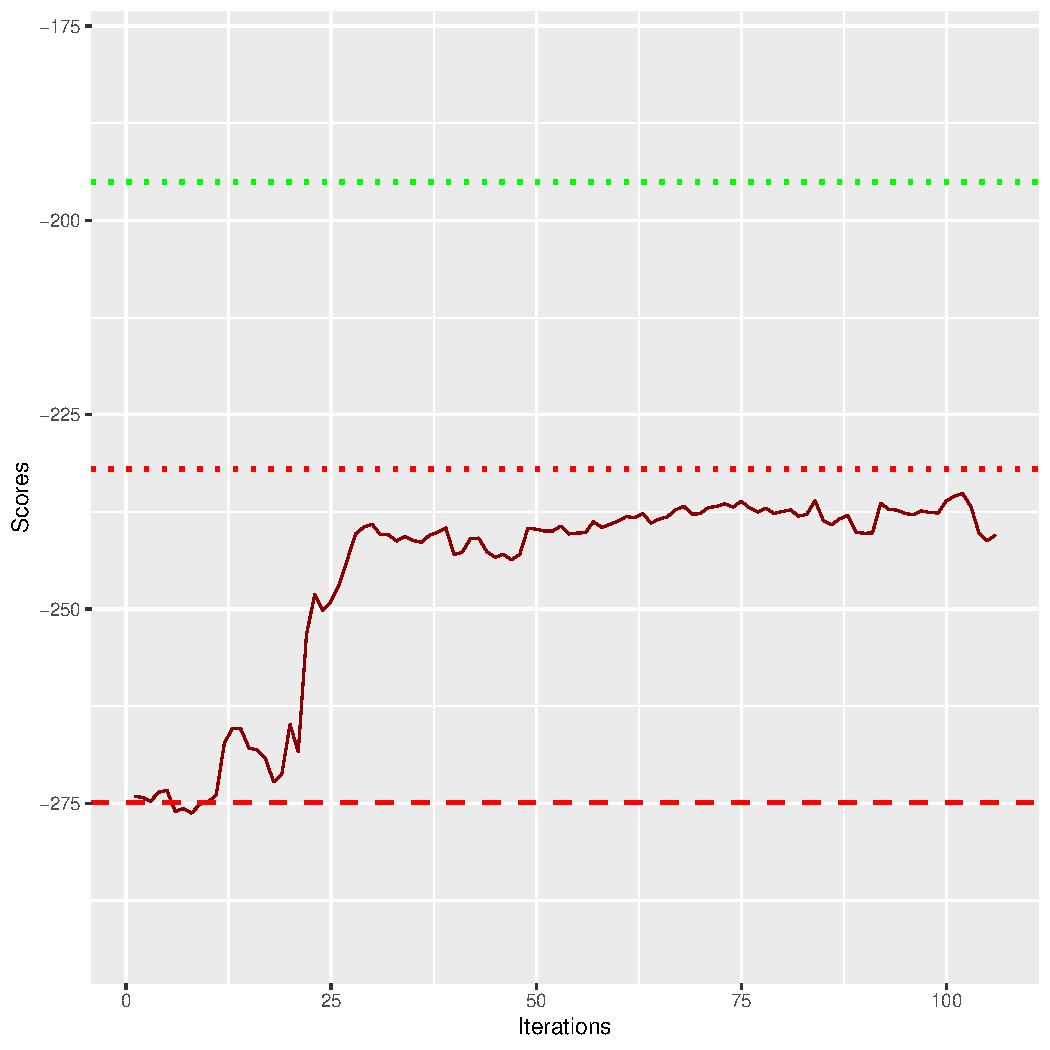
\includegraphics[scale = 0.4]{./figs/asia/v4/30/boundsEvolution-107.pdf} & 
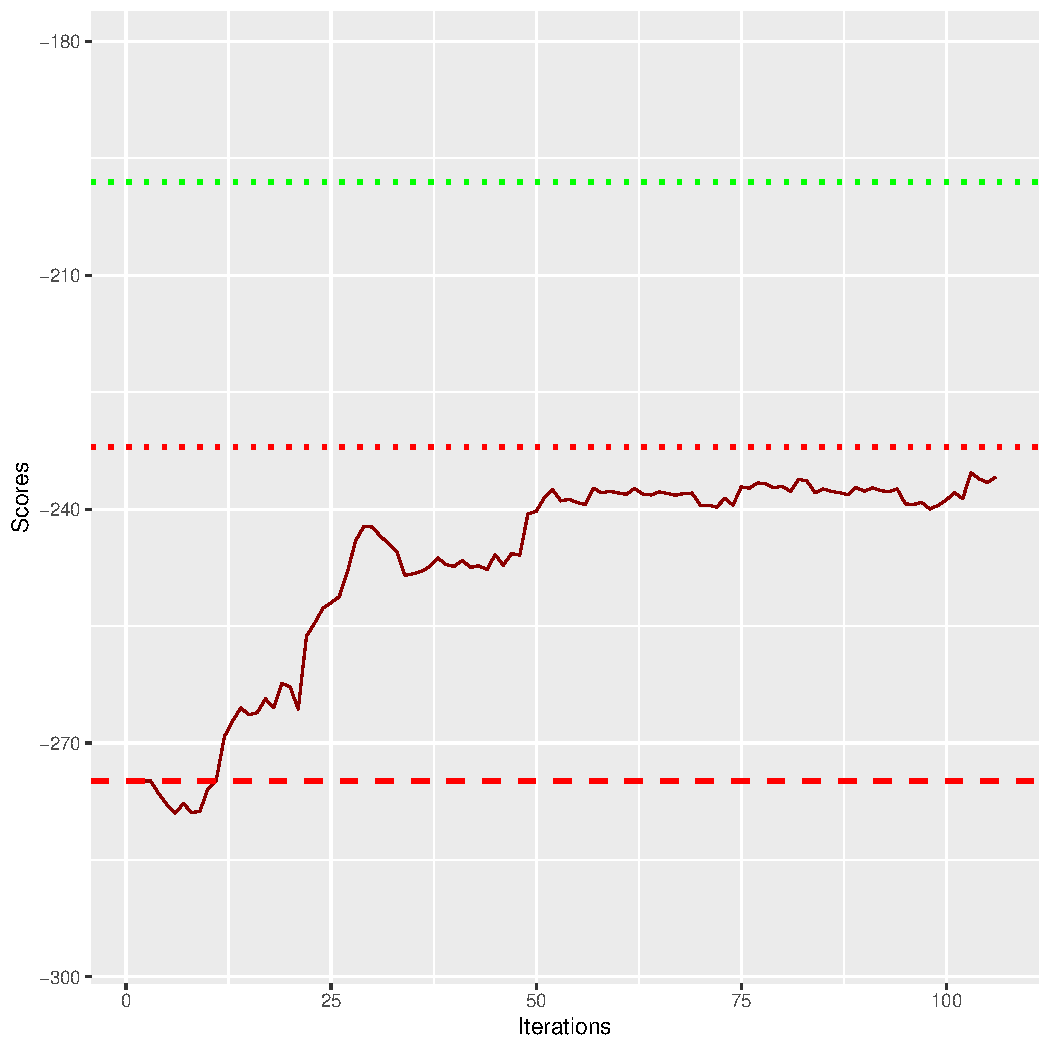
\includegraphics[scale = 0.4]{./figs/asia/v4/40/boundsEvolution-107.pdf} \\
\end{tabular}
\caption{Normal score for variant 4 with \textbf{np =  10, 20, 30, 40}}
\end{table}

\begin{table}[h!]
\begin{tabular}{cc}
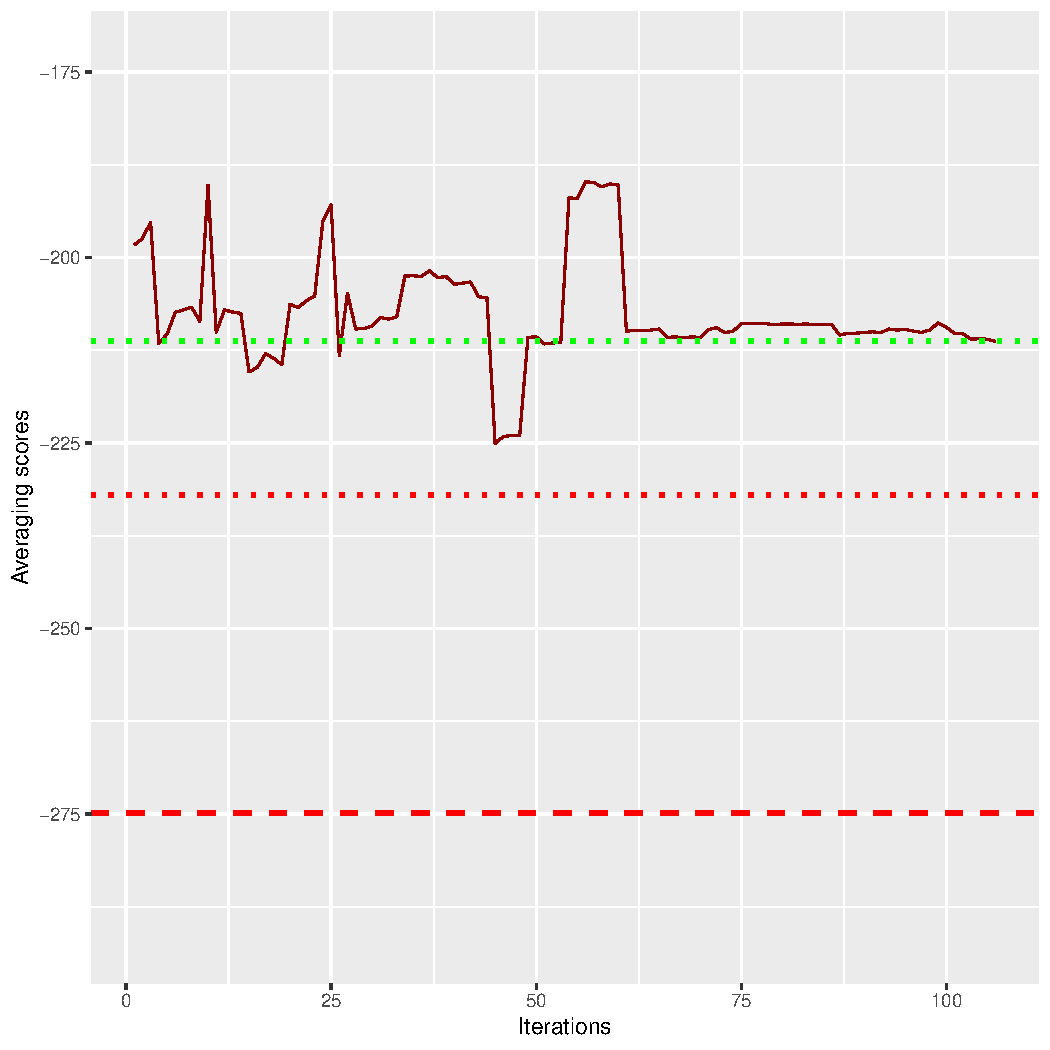
\includegraphics[scale = 0.4]{./figs/asia/v4/10/avgBoundsEvolution-107.pdf} & 
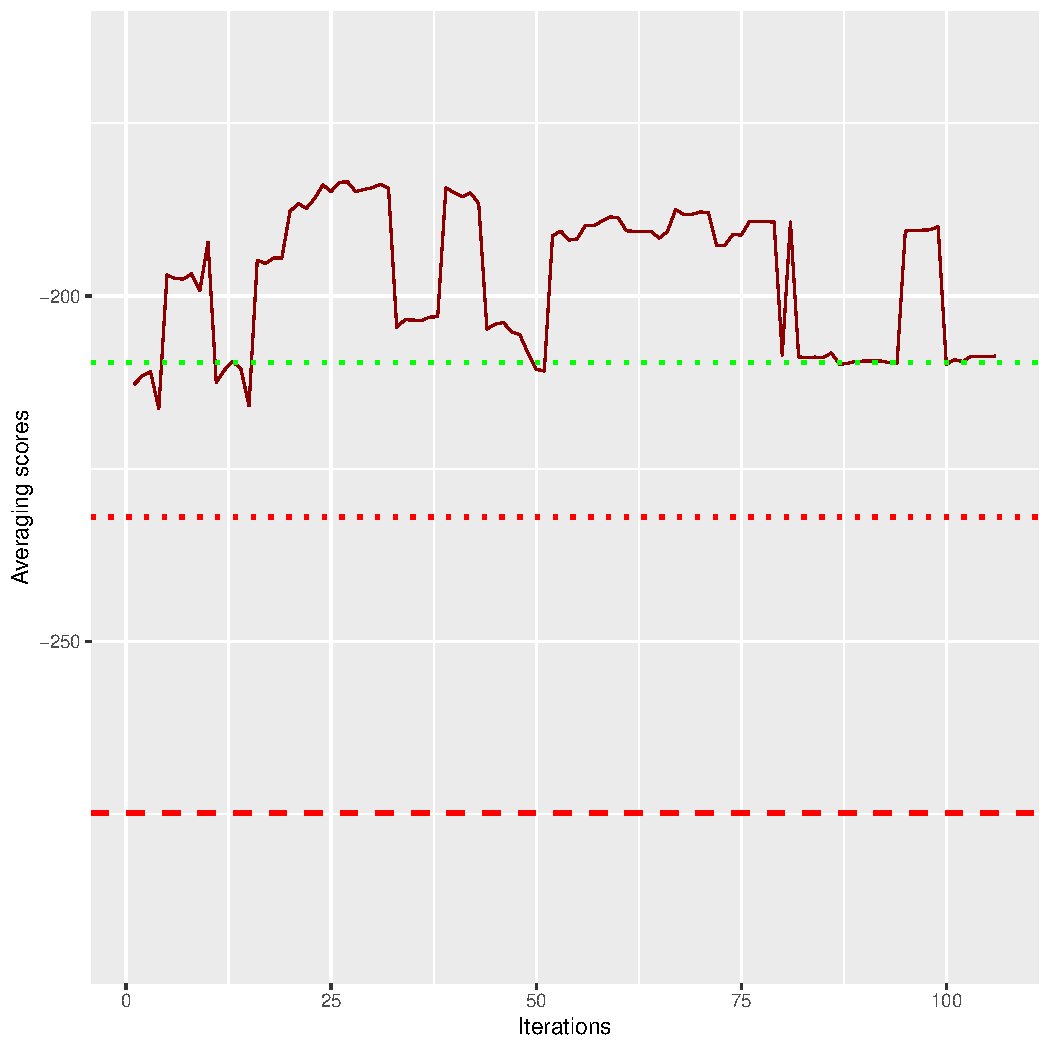
\includegraphics[scale = 0.4]{./figs/asia/v4/20/avgBoundsEvolution-107.pdf} \\
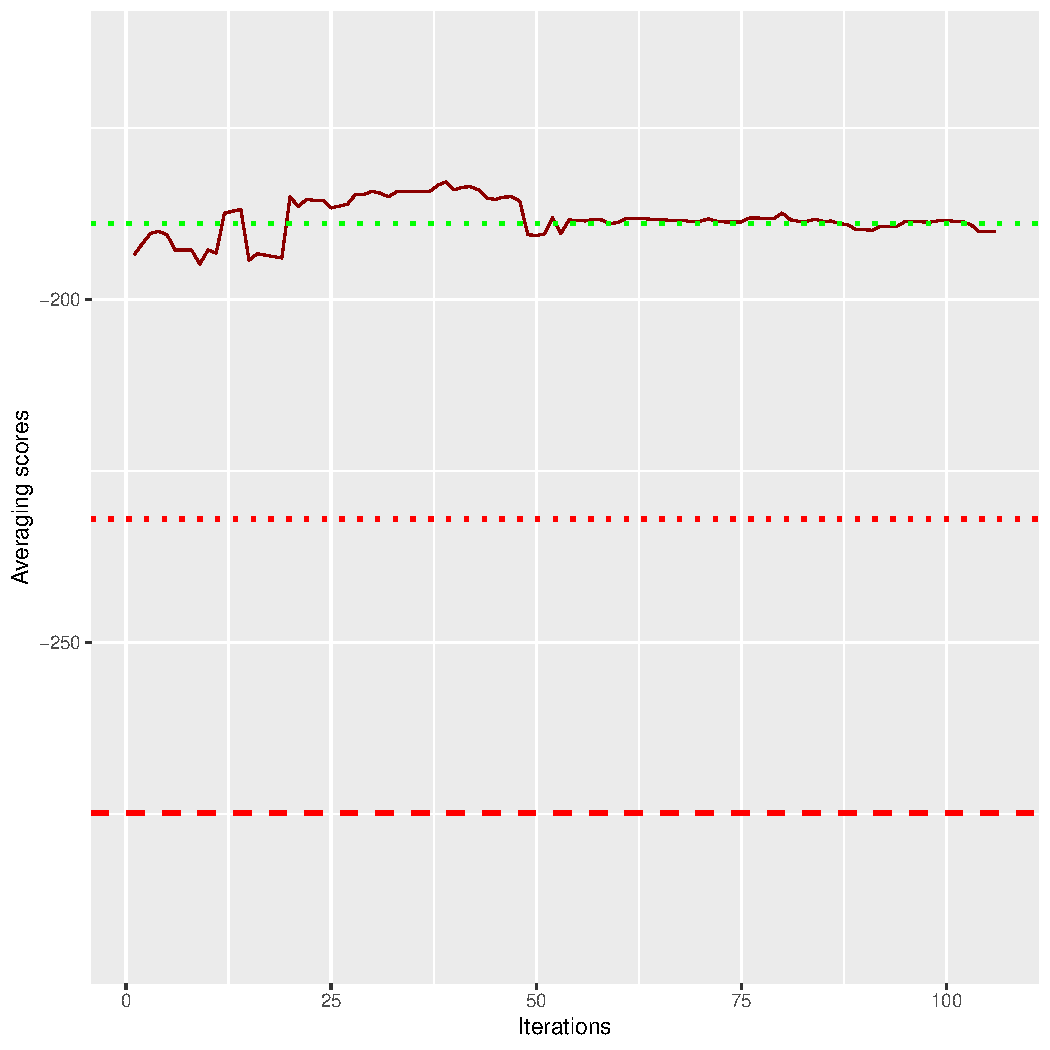
\includegraphics[scale = 0.4]{./figs/asia/v4/30/avgBoundsEvolution-107.pdf} & 
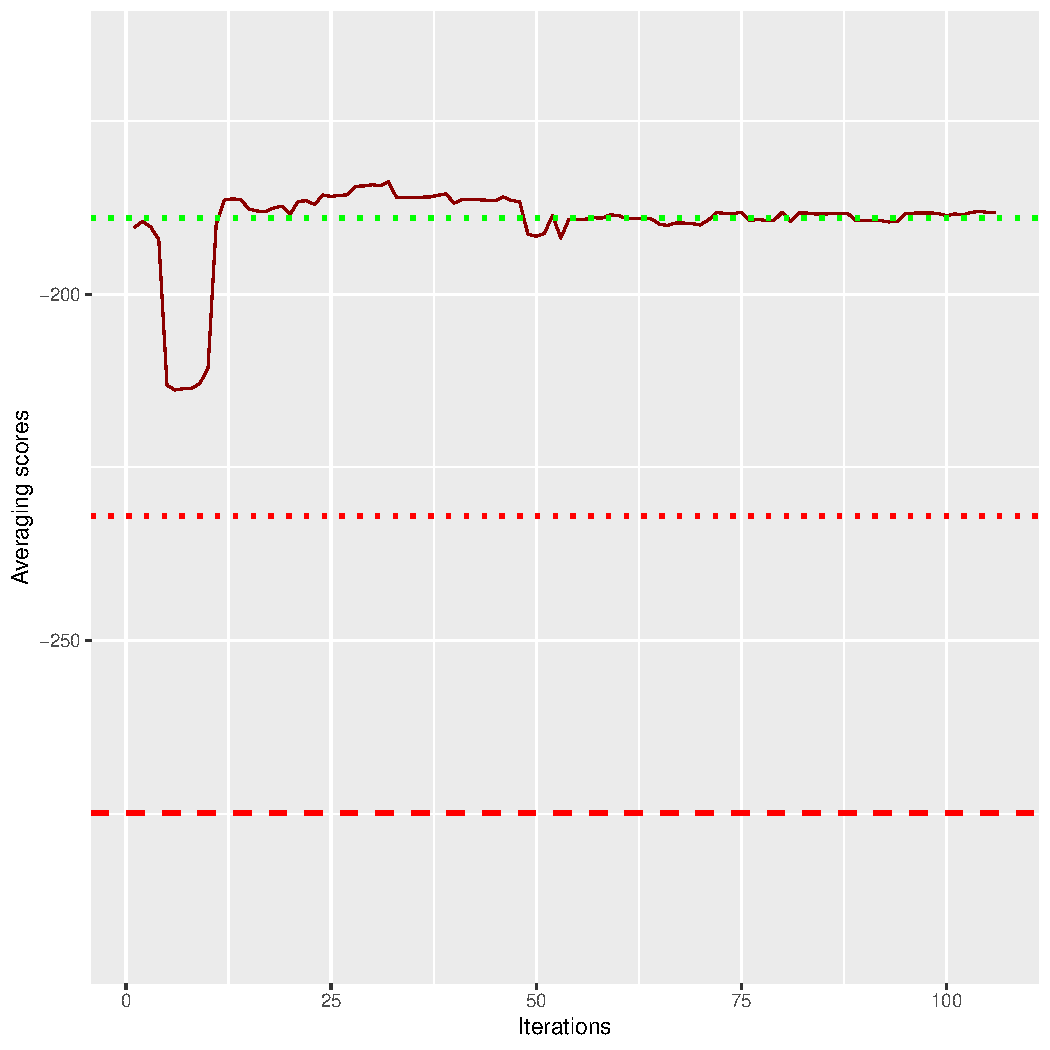
\includegraphics[scale = 0.4]{./figs/asia/v4/40/avgBoundsEvolution-107.pdf} \\
\end{tabular}
\caption{Averaging score for variant 4 with \textbf{np =  10, 20, 30, 40}}
\end{table}

\begin{table}[h!]
\begin{tabular}{cc}
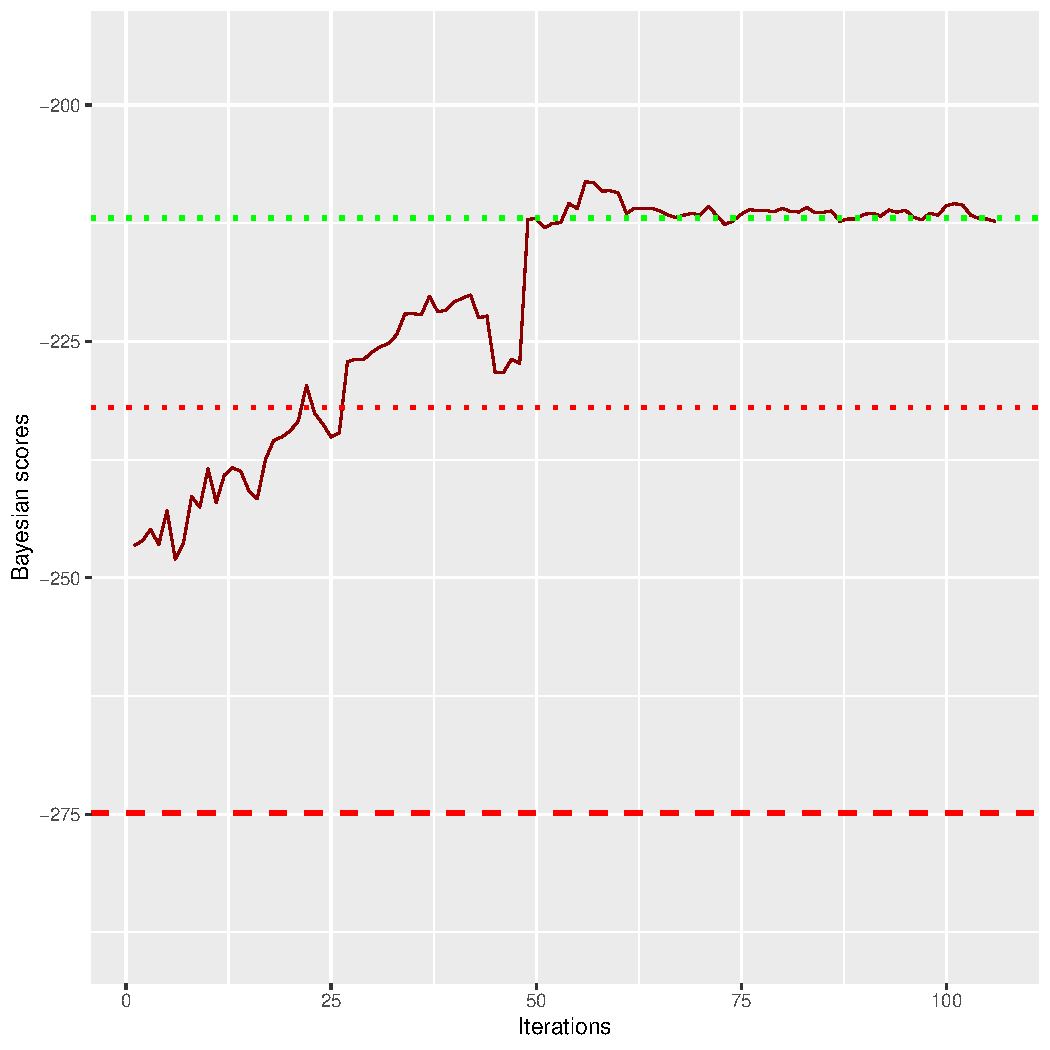
\includegraphics[scale = 0.4]{./figs/asia/v4/10/bayBoundsEvolution-107.pdf} & 
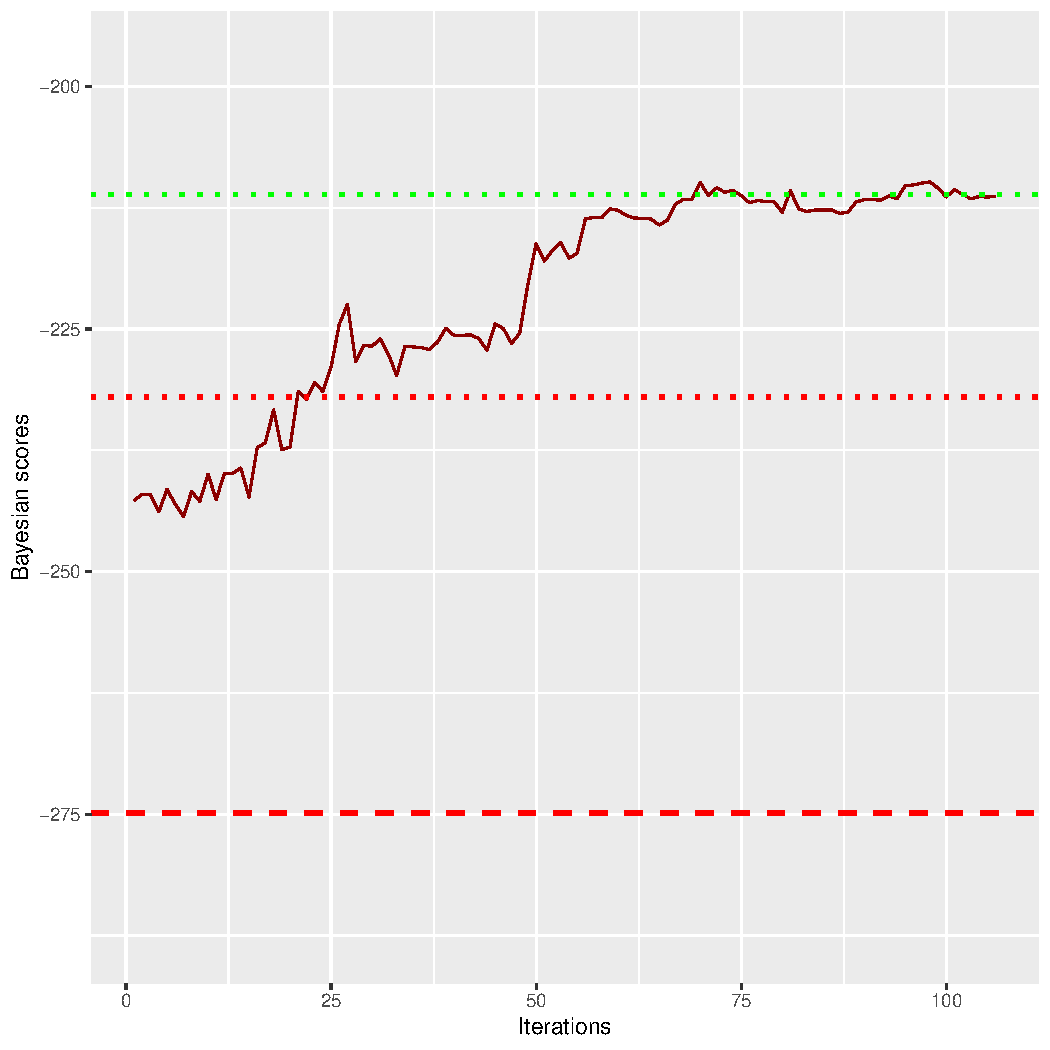
\includegraphics[scale = 0.4]{./figs/asia/v4/20/bayBoundsEvolution-107.pdf} \\
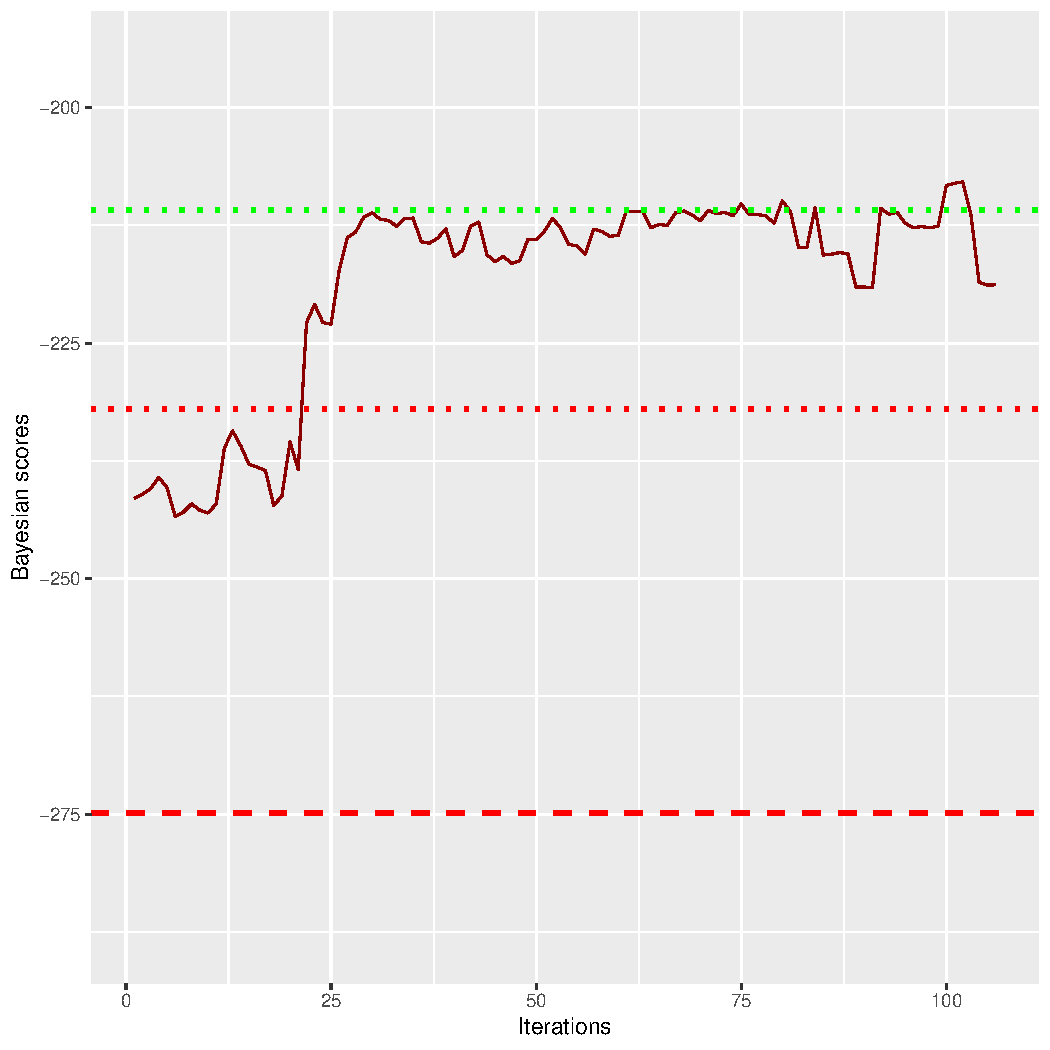
\includegraphics[scale = 0.4]{./figs/asia/v4/30/bayBoundsEvolution-107.pdf} & 
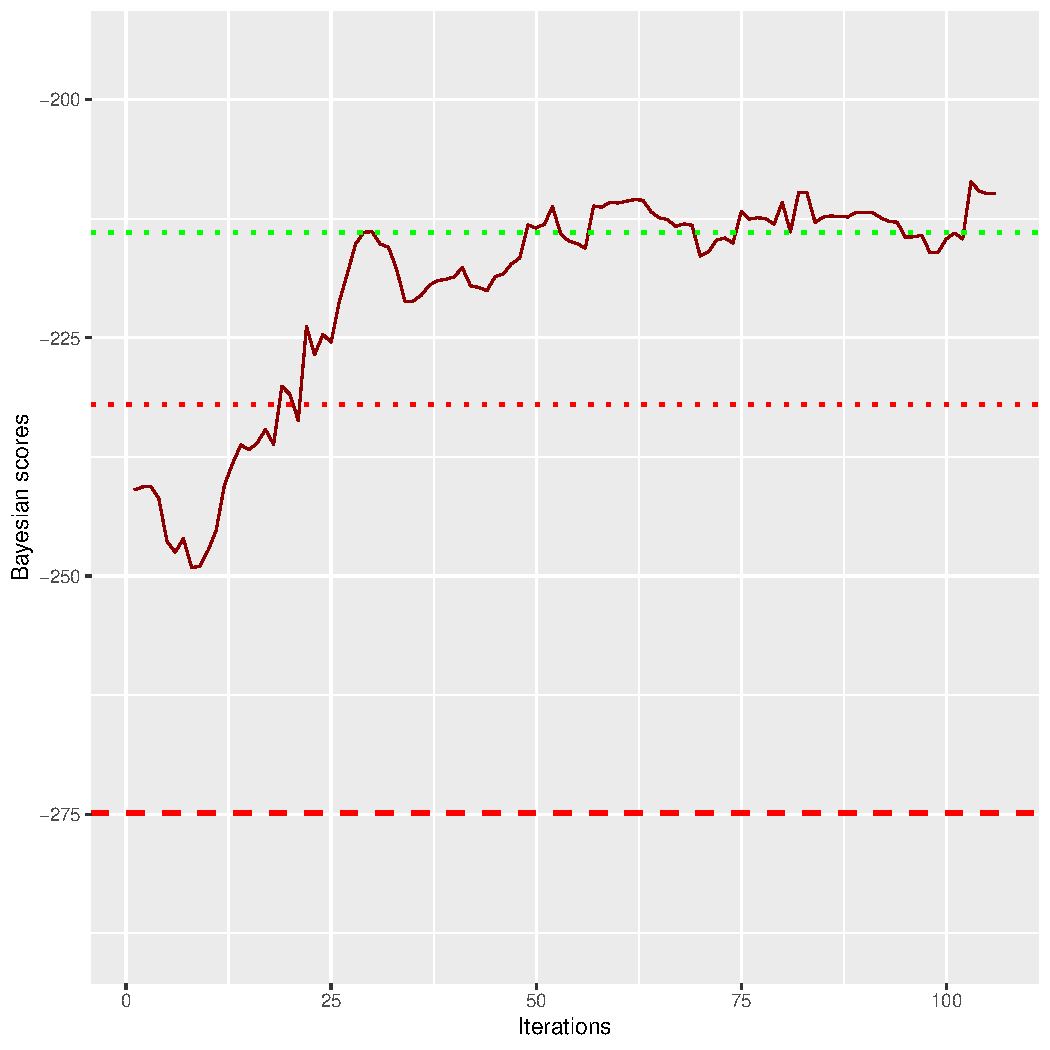
\includegraphics[scale = 0.4]{./figs/asia/v4/40/bayBoundsEvolution-107.pdf} \\
\end{tabular}
\caption{Bayesian score for variant 4 with \textbf{np =  10, 20, 30, 40}}
\end{table}

\clearpage

\subsection{Graphics of evolution for variant 5}

\begin{table}[h!]
\begin{tabular}{cc}
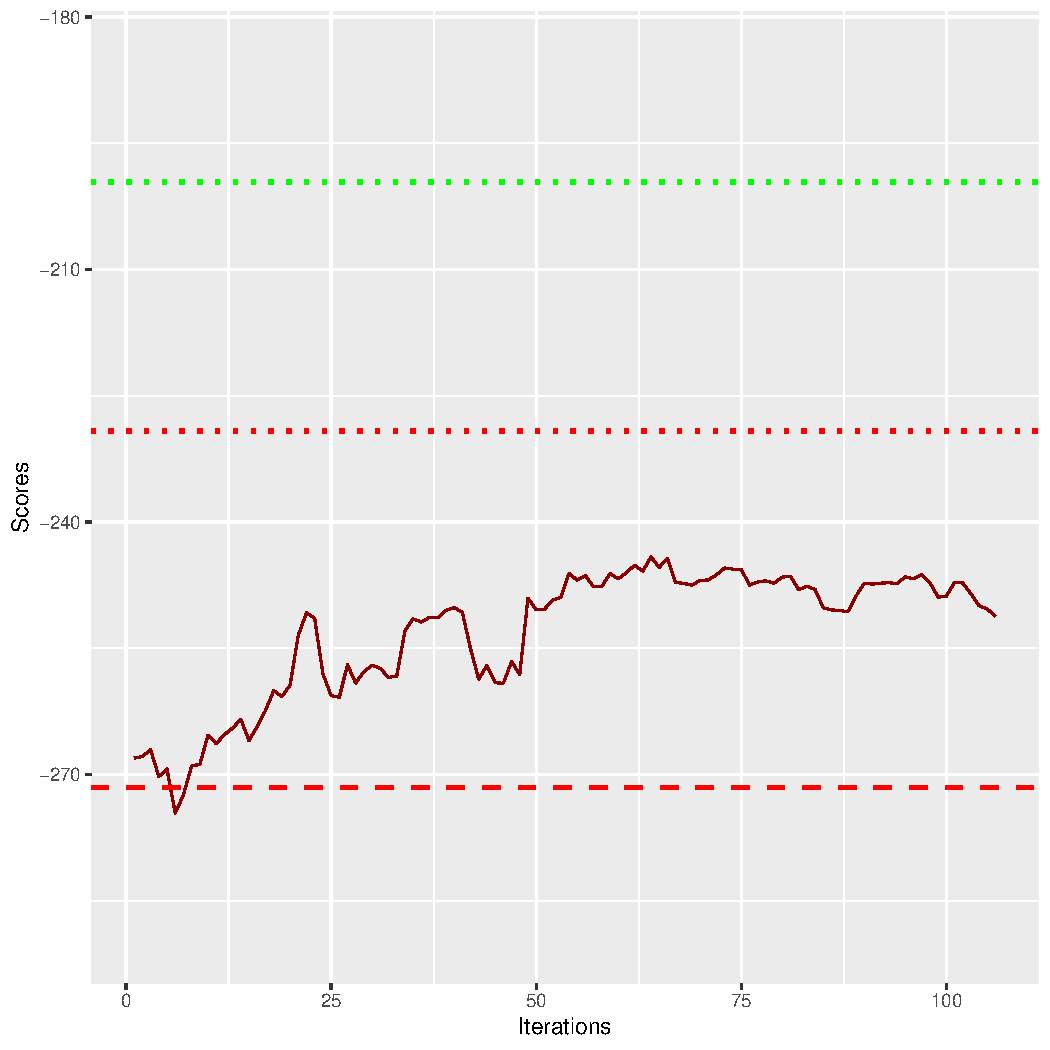
\includegraphics[scale = 0.4]{./figs/asia/v5/10/boundsEvolution-107.pdf} & 
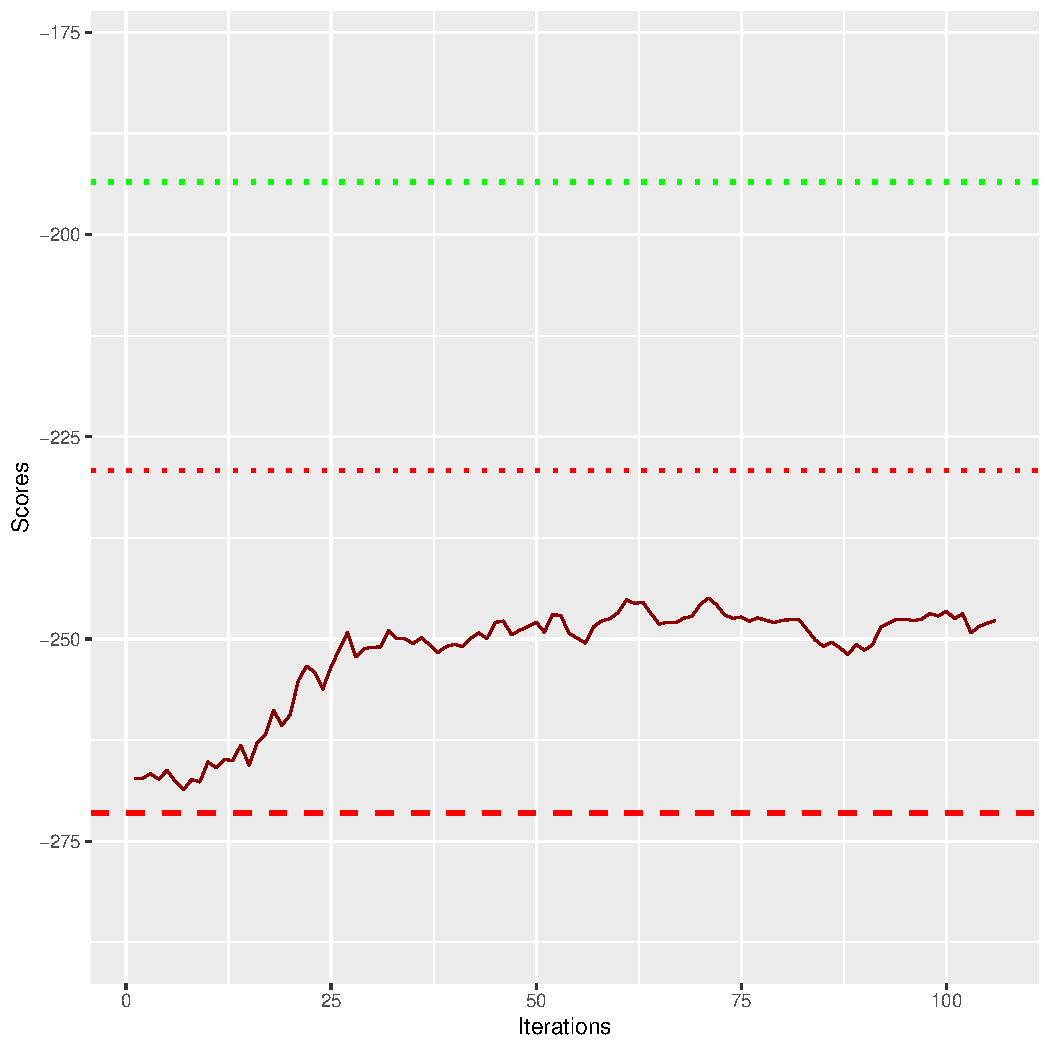
\includegraphics[scale = 0.4]{./figs/asia/v5/20/boundsEvolution-107.pdf} \\
\includegraphics[scale = 0.4]{./figs/asia/v5/30/boundsEvolution-107.pdf} & 
\includegraphics[scale = 0.4]{./figs/asia/v5/40/boundsEvolution-107.pdf} \\
\end{tabular}
\caption{Normal score for variant 5 with \textbf{np =  10, 20, 30, 40}}
\end{table}

\begin{table}[h!]
\begin{tabular}{cc}
\includegraphics[scale = 0.4]{./figs/asia/v5/10/avgBoundsEvolution-107.pdf} & 
\includegraphics[scale = 0.4]{./figs/asia/v5/20/avgBoundsEvolution-107.pdf} \\
\includegraphics[scale = 0.4]{./figs/asia/v5/30/avgBoundsEvolution-107.pdf} & 
\includegraphics[scale = 0.4]{./figs/asia/v5/40/avgBoundsEvolution-107.pdf} \\
\end{tabular}
\caption{Averaging score for variant 5 with \textbf{np =  10, 20, 30, 40}}
\end{table}

\begin{table}[h!]
\begin{tabular}{cc}
\includegraphics[scale = 0.4]{./figs/asia/v5/10/bayBoundsEvolution-107.pdf} & 
\includegraphics[scale = 0.4]{./figs/asia/v5/20/bayBoundsEvolution-107.pdf} \\
\includegraphics[scale = 0.4]{./figs/asia/v5/30/bayBoundsEvolution-107.pdf} & 
\includegraphics[scale = 0.4]{./figs/asia/v5/40/bayBoundsEvolution-107.pdf} \\
\end{tabular}
\caption{Bayesian score for variant 5 with \textbf{np =  10, 20, 30, 40}}
\end{table}

\clearpage

\section{Alarm network}

Configuration for \textbf{alarm}:

\begin{itemize}
\item number of nodes: 37
\item number of arcs: 46
\item number of parameters: 509
\item average degree: 2.49
\item maximum in-degree: 4
\item number of samples of tain dataset: 3500
\item number of samples of test dataset: 10000
\item number of iterations: 3500
\item parent sets size: \{30, 50, 70, 90\}
\end{itemize}

\begin{scriptsize}
\begin{center}
\begin{tabular}{cc|cc|cc|cc|cc|cc}
 & & \multicolumn{2}{c}{V1} & \multicolumn{2}{c}{V2} & \multicolumn{2}{c}{V3} & \multicolumn{2}{c}{V4} & \multicolumn{2}{c}{V5} \\
  & train & test & train & test  & train & test  & train & test  & train & test  \\
  \multicolumn{2}{l|}{bnlearn} & -6900 & -6577 & -7042 & -6738  & -7026  & -6712  & -7080  & -6730  & -7188  & -6651  \\\hline\hline
       \multirow{3}{*}{np = 30} & normal & -5685  & -5265  & -5882  & -5345  & -5759  & \textbf{-5220 } & -5783  & -5192  & -5918  & -5284  \\
                                                    & avg        & & -5214  & & -5333  & & \textbf{-5217  }& & -5138  & & -5193 \\
                                                    & bay        & & -5293  & & -5382  & & \textbf{-5256 } & & -5224  & & -5318  \\\cline{1-12}
    \multirow{3}{*}{np = 50} & normal & -5693  & -5251  & -5977  &-5394  & -5732 & -5229  & -5867  & -5301  & -6017  & -5359 \\
    												& avg        & & -5210  & & -5348  & & -5233  & & -5212  & & -5235 \\
                                                     & bay        & & -5281  & & -5428  & & -5264  & & -5332  & & -5392 \\\cline{1-12}
  \multirow{3}{*}{np = 70} & normal & -5713  & -5251  & -5870  & \textbf{-5317  }& -5769  & -5286  & -5843  & -5239  & -5933  & -5311 \\
    												   & avg        & & -5127  & & \textbf{-5291 } & & -5264  & & -5107  & & -5153 \\
                                                       & bay        & & -5280  & & \textbf{-5353 } & & -5319  & &  -5272  & & -5343 \\\cline{1-12}
 \multirow{3}{*}{np = 90} & normal & -5697  & -5257  & -5950  & -5364  & -5727  & -5247  & -5878  & -5287  & -6000  & -5367  \\
    												    & avg        & & -5180  & & -5214 & & -5232  & & -5124  & & -5234 \\
                                                        & bay        & & -5289  & & -5403 & & -5282  & & -5321  & & -5401 \\                                                                                                                
\end{tabular}
\end{center}
\end{scriptsize}

\newpage

\subsection{Graphics of evolution for variant 1}

\begin{table}[h!]
\begin{tabular}{cc}
\includegraphics[scale = 0.4]{./figs/alarm/v1/30/boundsEvolution-3502.pdf} & 
\includegraphics[scale = 0.4]{./figs/alarm/v1/50/boundsEvolution-3502.pdf} \\
\includegraphics[scale = 0.4]{./figs/alarm/v1/70/boundsEvolution-3502.pdf} & 
\includegraphics[scale = 0.4]{./figs/alarm/v1/90/boundsEvolution-3502.pdf} \\
\end{tabular}
\caption{Normal score for variant 1 with \textbf{np =  30, 50, 70, 90 }}
\end{table}

\begin{table}[h!]
\begin{tabular}{cc}
\includegraphics[scale = 0.4]{./figs/alarm/v1/30/avgBoundsEvolution-3502.pdf} & 
\includegraphics[scale = 0.4]{./figs/alarm/v1/50/avgBoundsEvolution-3502.pdf} \\
\includegraphics[scale = 0.4]{./figs/alarm/v1/70/avgBoundsEvolution-3502.pdf} & 
\includegraphics[scale = 0.4]{./figs/alarm/v1/90/avgBoundsEvolution-3502.pdf} \\
\end{tabular}
\caption{Averaging score for variant 1 with \textbf{np =  30, 50, 70, 90 }}
\end{table}

\begin{table}[h!]
\begin{tabular}{cc}
\includegraphics[scale = 0.4]{./figs/alarm/v1/30/bayBoundsEvolution-3502.pdf} & 
\includegraphics[scale = 0.4]{./figs/alarm/v1/50/bayBoundsEvolution-3502.pdf} \\
\includegraphics[scale = 0.4]{./figs/alarm/v1/70/bayBoundsEvolution-3502.pdf} & 
\includegraphics[scale = 0.4]{./figs/alarm/v1/90/bayBoundsEvolution-3502.pdf} \\
\end{tabular}
\caption{Bayesian score for variant 1 with \textbf{np =  30, 50, 70, 90 }}
\end{table}

\clearpage

\subsection{Graphics of evolution for variant 2}

\begin{table}[h!]
\begin{tabular}{cc}
\includegraphics[scale = 0.4]{./figs/alarm/v2/30/boundsEvolution-3502.pdf} & 
\includegraphics[scale = 0.4]{./figs/alarm/v2/50/boundsEvolution-3502.pdf} \\
\includegraphics[scale = 0.4]{./figs/alarm/v2/70/boundsEvolution-3502.pdf} & 
\includegraphics[scale = 0.4]{./figs/alarm/v2/90/boundsEvolution-3502.pdf} \\
\end{tabular}
\caption{Normal score for variant 2 with \textbf{np =  30, 50, 70, 90 }}
\end{table}

\begin{table}[h!]
\begin{tabular}{cc}
\includegraphics[scale = 0.4]{./figs/alarm/v2/30/avgBoundsEvolution-3502.pdf} & 
\includegraphics[scale = 0.4]{./figs/alarm/v2/50/avgBoundsEvolution-3502.pdf} \\
\includegraphics[scale = 0.4]{./figs/alarm/v2/70/avgBoundsEvolution-3502.pdf} & 
\includegraphics[scale = 0.4]{./figs/alarm/v2/90/avgBoundsEvolution-3502.pdf} \\
\end{tabular}
\caption{Averaging score for variant 2 with \textbf{np =  30, 50, 70, 90 }}
\end{table}

\begin{table}[h!]
\begin{tabular}{cc}
\includegraphics[scale = 0.4]{./figs/alarm/v2/30/bayBoundsEvolution-3502.pdf} & 
\includegraphics[scale = 0.4]{./figs/alarm/v2/50/bayBoundsEvolution-3502.pdf} \\
\includegraphics[scale = 0.4]{./figs/alarm/v2/70/bayBoundsEvolution-3502.pdf} & 
\includegraphics[scale = 0.4]{./figs/alarm/v2/90/bayBoundsEvolution-3502.pdf} \\
\end{tabular}
\caption{Bayesian score for variant 2 with \textbf{np =  30, 50, 70, 90 }}
\end{table}

\clearpage

\subsection{Graphics of evolution for variant 3}

\begin{table}[h!]
\begin{tabular}{cc}
\includegraphics[scale = 0.4]{./figs/alarm/v3/30/boundsEvolution-3502.pdf} & 
\includegraphics[scale = 0.4]{./figs/alarm/v3/50/boundsEvolution-3502.pdf} \\
\includegraphics[scale = 0.4]{./figs/alarm/v3/70/boundsEvolution-3502.pdf} & 
\includegraphics[scale = 0.4]{./figs/alarm/v3/90/boundsEvolution-3502.pdf} \\
\end{tabular}
\caption{Normal score for variant 3 with \textbf{np =  30, 50, 70, 90 }}
\end{table}

\begin{table}[h!]
\begin{tabular}{cc}
\includegraphics[scale = 0.4]{./figs/alarm/v3/30/avgBoundsEvolution-3502.pdf} & 
\includegraphics[scale = 0.4]{./figs/alarm/v3/50/avgBoundsEvolution-3502.pdf} \\
\includegraphics[scale = 0.4]{./figs/alarm/v3/70/avgBoundsEvolution-3502.pdf} & 
\includegraphics[scale = 0.4]{./figs/alarm/v3/90/avgBoundsEvolution-3502.pdf} \\
\end{tabular}
\caption{Averaging score for variant 3 with \textbf{np =  30, 50, 70, 90 }}
\end{table}

\begin{table}[h!]
\begin{tabular}{cc}
\includegraphics[scale = 0.4]{./figs/alarm/v3/30/bayBoundsEvolution-3502.pdf} & 
\includegraphics[scale = 0.4]{./figs/alarm/v3/50/bayBoundsEvolution-3502.pdf} \\
\includegraphics[scale = 0.4]{./figs/alarm/v3/70/bayBoundsEvolution-3502.pdf} & 
\includegraphics[scale = 0.4]{./figs/alarm/v3/90/bayBoundsEvolution-3502.pdf} \\
\end{tabular}
\caption{Bayesian score for variant 3 with \textbf{np =  30, 50, 70, 90 }}
\end{table}

\clearpage

\subsection{Graphics of evolution for variant 4}

\begin{table}[h!]
\begin{tabular}{cc}
\includegraphics[scale = 0.4]{./figs/alarm/v4/30/boundsEvolution-3502.pdf} & 
\includegraphics[scale = 0.4]{./figs/alarm/v4/50/boundsEvolution-3502.pdf} \\
\includegraphics[scale = 0.4]{./figs/alarm/v4/70/boundsEvolution-3502.pdf} & 
\includegraphics[scale = 0.4]{./figs/alarm/v4/90/boundsEvolution-3502.pdf} \\
\end{tabular}
\caption{Normal score for variant 4 with \textbf{np =  30, 50, 70, 90 }}
\end{table}

\begin{table}[h!]
\begin{tabular}{cc}
\includegraphics[scale = 0.4]{./figs/alarm/v4/30/avgBoundsEvolution-3502.pdf} & 
\includegraphics[scale = 0.4]{./figs/alarm/v4/50/avgBoundsEvolution-3502.pdf} \\
\includegraphics[scale = 0.4]{./figs/alarm/v4/70/avgBoundsEvolution-3502.pdf} & 
\includegraphics[scale = 0.4]{./figs/alarm/v4/90/avgBoundsEvolution-3502.pdf} \\
\end{tabular}
\caption{Averaging score for variant 4 with \textbf{np =  30, 50, 70, 90 }}
\end{table}

\begin{table}[h!]
\begin{tabular}{cc}
\includegraphics[scale = 0.4]{./figs/alarm/v4/30/bayBoundsEvolution-3502.pdf} & 
\includegraphics[scale = 0.4]{./figs/alarm/v4/50/bayBoundsEvolution-3502.pdf} \\
\includegraphics[scale = 0.4]{./figs/alarm/v4/70/bayBoundsEvolution-3502.pdf} & 
\includegraphics[scale = 0.4]{./figs/alarm/v4/90/bayBoundsEvolution-3502.pdf} \\
\end{tabular}
\caption{Bayesian score for variant 4 with \textbf{np =  30, 50, 70, 90 }}
\end{table}

\clearpage

\subsection{Graphics of evolution for variant 5}

\begin{table}[h!]
\begin{tabular}{cc}
\includegraphics[scale = 0.4]{./figs/alarm/v5/30/boundsEvolution-3502.pdf} & 
\includegraphics[scale = 0.4]{./figs/alarm/v5/50/boundsEvolution-3502.pdf} \\
\includegraphics[scale = 0.4]{./figs/alarm/v5/70/boundsEvolution-3502.pdf} & 
\includegraphics[scale = 0.4]{./figs/alarm/v5/90/boundsEvolution-3502.pdf} \\
\end{tabular}
\caption{Normal score for variant 5 with \textbf{np =  30, 50, 70, 90 }}
\end{table}

\begin{table}[h!]
\begin{tabular}{cc}
\includegraphics[scale = 0.4]{./figs/alarm/v5/30/avgBoundsEvolution-3502.pdf} & 
\includegraphics[scale = 0.4]{./figs/alarm/v5/50/avgBoundsEvolution-3502.pdf} \\
\includegraphics[scale = 0.4]{./figs/alarm/v5/70/avgBoundsEvolution-3502.pdf} & 
\includegraphics[scale = 0.4]{./figs/alarm/v5/90/avgBoundsEvolution-3502.pdf} \\
\end{tabular}
\caption{Averaging score for variant 5 with \textbf{np =  30, 50, 70, 90 }}
\end{table}

\begin{table}[h!]
\begin{tabular}{cc}
\includegraphics[scale = 0.4]{./figs/alarm/v5/30/bayBoundsEvolution-3502.pdf} & 
\includegraphics[scale = 0.4]{./figs/alarm/v5/50/bayBoundsEvolution-3502.pdf} \\
\includegraphics[scale = 0.4]{./figs/alarm/v5/70/bayBoundsEvolution-3502.pdf} & 
\includegraphics[scale = 0.4]{./figs/alarm/v5/90/bayBoundsEvolution-3502.pdf} \\
\end{tabular}
\caption{Bayesian score for variant 5 with \textbf{np =  30, 50, 70, 90 }}
\end{table}

\clearpage

\section{Hepar2}

Configuration for \textbf{hepar2}:

\begin{itemize}
\item number of nodes: 70
\item number of arcs: 123
\item number of parameters: 1453
\item average degree: 3.51
\item maximum in-degree: 6
\item number of samples of train dataset: 3000
\item number of samples of test dataset: 10000
\item number of iterations: 10350
\item parent sets size: \{25, 50, 75, 100\}
\end{itemize}

\begin{scriptsize}
\begin{center}
\begin{tabular}{cc|cc|cc|cc|cc|cc}
 & & \multicolumn{2}{c}{V1} & \multicolumn{2}{c}{V2} & \multicolumn{2}{c}{V3} & \multicolumn{2}{c}{V4} & \multicolumn{2}{c}{V5} \\
  & train & test & train & test  & train & test  & train & test  & train & test  \\
  \multicolumn{2}{l|}{bnlearn} & -97973  & -98139  & -98361  & -98190  & -98506  & -98115  & -98079  & -98117  & -98614  & -98113  \\\hline\hline
       \multirow{3}{*}{np = 25} & normal & -97650 & -97692 & -97968  & -97727  & - 98232 & - 97793 & -97607  & -97648  & -98258  & -97864  \\
                                                    & avg             & & -997572            & & -97317                 & & -97150                   & & -97554                 & & -96691 \\
                                                    & bay             & & -97779              & & -97812                 & & -97879                   & & - 97736                & & - 97594 \\\cline{1-12}
    \multirow{3}{*}{np = 50} & normal &-97705 & -97800  & -98054  &-97794  & -98097 & -97704 & -97839  & -97858  & -98276  & -97697 \\
    												& avg        & & -97597                 & & -97740                 & & -97494                & & -97795                & & -97463 \\
                                                     & bay        & & -97891                & & -97882                 & & -97784                & & - 97947                & & -97779 \\\cline{1-12}
  \multirow{3}{*}{np = 75} & normal & -97662 & -97718  & -97998  & -97741  &  -98177 & -97776  & -97715  & -97720  & -98319  & -97764 \\
    												   & avg        & & -97426             & & -97109                 & & -97483                  & & -97460                 & & -97515 \\
                                                       & bay        & & -97804              & & -97828                & & -97860                  & &  -97806                & & -97849 \\\cline{1-12}
 \multirow{3}{*}{np = 100} & normal & -97723  & -97789  & -98046  & -97775  & -98199  & -97815  & -97652  & -97657  & -98233  & -97790  \\
    												    & avg        & & -97581              & & -97503                  & & -97297                 & & -97186                  & & -97540 \\
                                                        & bay        & & -97876              & & -97860                  & & -97897                 & & -97742                 & & -97875 \\                                                                                                                
\end{tabular}
\end{center}
\end{scriptsize}

\newpage

\subsection{Graphics of evolution for variant 1}

\begin{table}[h!]
\begin{tabular}{cc}
\includegraphics[scale = 0.4]{./figs/hepar2/v1/25/boundsEvolution-10352.pdf} & 
\includegraphics[scale = 0.4]{./figs/hepar2/v1/50/boundsEvolution-10352.pdf} \\
\includegraphics[scale = 0.4]{./figs/hepar2/v1/75/boundsEvolution-10352.pdf} & 
\includegraphics[scale = 0.4]{./figs/hepar2/v1/100/boundsEvolution-10352.pdf} \\
\end{tabular}
\caption{Normal score for variant 1 with \textbf{np =  25, 50, 75, 100 }}
\end{table}

\begin{table}[h!]
\begin{tabular}{cc}
\includegraphics[scale = 0.4]{./figs/hepar2/v1/25/avgBoundsEvolution-10352.pdf} & 
\includegraphics[scale = 0.4]{./figs/hepar2/v1/50/avgBoundsEvolution-10352.pdf} \\
\includegraphics[scale = 0.4]{./figs/hepar2/v1/75/avgBoundsEvolution-10352.pdf} & 
\includegraphics[scale = 0.4]{./figs/hepar2/v1/100/avgBoundsEvolution-10352.pdf} \\
\end{tabular}
\caption{Averaging score for variant 1 with \textbf{np =  25, 50, 75, 100}}
\end{table}

\begin{table}[h!]
\begin{tabular}{cc}
\includegraphics[scale = 0.4]{./figs/hepar2/v1/25/bayBoundsEvolution-10352.pdf} & 
\includegraphics[scale = 0.4]{./figs/hepar2/v1/50/bayBoundsEvolution-10352.pdf} \\
\includegraphics[scale = 0.4]{./figs/hepar2/v1/75/bayBoundsEvolution-10352.pdf} & 
\includegraphics[scale = 0.4]{./figs/hepar2/v1/100/bayBoundsEvolution-10352.pdf} \\
\end{tabular}
\caption{Bayesian score for variant 1 with \textbf{np =  25, 50, 75, 100}}
\end{table}

\clearpage

\subsection{Graphics of evolution for variant 2}

\begin{table}[h!]
\begin{tabular}{cc}
\includegraphics[scale = 0.4]{./figs/hepar2/v2/25/boundsEvolution-10352.pdf} & 
\includegraphics[scale = 0.4]{./figs/hepar2/v2/50/boundsEvolution-10352.pdf} \\
\includegraphics[scale = 0.4]{./figs/hepar2/v2/75/boundsEvolution-10352.pdf} & 
\includegraphics[scale = 0.4]{./figs/hepar2/v2/100/boundsEvolution-10352.pdf} \\
\end{tabular}
\caption{Normal score for variant 2 with \textbf{np =  25, 50, 75, 100}}
\end{table}

\begin{table}[h!]
\begin{tabular}{cc}
\includegraphics[scale = 0.4]{./figs/hepar2/v2/25/avgBoundsEvolution-10352.pdf} & 
\includegraphics[scale = 0.4]{./figs/hepar2/v2/50/avgBoundsEvolution-10352.pdf} \\
\includegraphics[scale = 0.4]{./figs/hepar2/v2/75/avgBoundsEvolution-10352.pdf} & 
\includegraphics[scale = 0.4]{./figs/hepar2/v2/100/avgBoundsEvolution-10352.pdf} \\
\end{tabular}
\caption{Averaging score for variant 2 with \textbf{np =  25, 50, 75, 100}}
\end{table}

\begin{table}[h!]
\begin{tabular}{cc}
\includegraphics[scale = 0.4]{./figs/hepar2/v2/25/bayBoundsEvolution-10352.pdf} & 
\includegraphics[scale = 0.4]{./figs/hepar2/v2/50/bayBoundsEvolution-10352.pdf} \\
\includegraphics[scale = 0.4]{./figs/hepar2/v2/75/bayBoundsEvolution-10352.pdf} & 
\includegraphics[scale = 0.4]{./figs/hepar2/v2/100/bayBoundsEvolution-10352.pdf} \\
\end{tabular}
\caption{Bayesian score for variant 2 with \textbf{np =  25, 50, 75, 100}}
\end{table}

\clearpage

\subsection{Graphics of evolution for variant 3}

\begin{table}[h!]
\begin{tabular}{cc}
\includegraphics[scale = 0.4]{./figs/hepar2/v3/25/boundsEvolution-10352.pdf} & 
\includegraphics[scale = 0.4]{./figs/hepar2/v3/50/boundsEvolution-10352.pdf} \\
\includegraphics[scale = 0.4]{./figs/hepar2/v3/75/boundsEvolution-10352.pdf} & 
\includegraphics[scale = 0.4]{./figs/hepar2/v3/100/boundsEvolution-10352.pdf} \\
\end{tabular}
\caption{Normal score for variant 3 with \textbf{np =  25, 50, 75, 100}}
\end{table}

\begin{table}[h!]
\begin{tabular}{cc}
\includegraphics[scale = 0.4]{./figs/hepar2/v3/25/avgBoundsEvolution-10352.pdf} & 
\includegraphics[scale = 0.4]{./figs/hepar2/v3/50/avgBoundsEvolution-10352.pdf} \\
\includegraphics[scale = 0.4]{./figs/hepar2/v3/75/avgBoundsEvolution-10352.pdf} & 
\includegraphics[scale = 0.4]{./figs/hepar2/v3/100/avgBoundsEvolution-10352.pdf} \\
\end{tabular}
\caption{Averaging score for variant 3 with \textbf{np =  25, 50, 75, 100}}
\end{table}

\begin{table}[h!]
\begin{tabular}{cc}
\includegraphics[scale = 0.4]{./figs/hepar2/v3/25/bayBoundsEvolution-10352.pdf} & 
\includegraphics[scale = 0.4]{./figs/hepar2/v3/50/bayBoundsEvolution-10352.pdf} \\
\includegraphics[scale = 0.4]{./figs/hepar2/v3/75/bayBoundsEvolution-10352.pdf} & 
\includegraphics[scale = 0.4]{./figs/hepar2/v3/100/bayBoundsEvolution-10352.pdf} \\
\end{tabular}
\caption{Bayesian score for variant 3 with \textbf{np =  25, 50, 75, 100}}
\end{table}

\clearpage

\subsection{Graphics of evolution for variant 4}

\begin{table}[h!]
\begin{tabular}{cc}
\includegraphics[scale = 0.4]{./figs/hepar2/v4/25/boundsEvolution-10352.pdf} & 
\includegraphics[scale = 0.4]{./figs/hepar2/v4/50/boundsEvolution-10352.pdf} \\
\includegraphics[scale = 0.4]{./figs/hepar2/v4/75/boundsEvolution-10352.pdf} & 
\includegraphics[scale = 0.4]{./figs/hepar2/v4/100/boundsEvolution-10352.pdf} \\
\end{tabular}
\caption{Normal score for variant 4 with \textbf{np =  25, 50, 75, 100}}
\end{table}

\begin{table}[h!]
\begin{tabular}{cc}
\includegraphics[scale = 0.4]{./figs/hepar2/v4/25/avgBoundsEvolution-10352.pdf} & 
\includegraphics[scale = 0.4]{./figs/hepar2/v4/50/avgBoundsEvolution-10352.pdf} \\
\includegraphics[scale = 0.4]{./figs/hepar2/v4/75/avgBoundsEvolution-10352.pdf} & 
\includegraphics[scale = 0.4]{./figs/hepar2/v4/100/avgBoundsEvolution-10352.pdf} \\
\end{tabular}
\caption{Averaging score for variant 4 with \textbf{np =  25, 50, 75, 100 }}
\end{table}

\begin{table}[h!]
\begin{tabular}{cc}
\includegraphics[scale = 0.4]{./figs/hepar2/v4/25/bayBoundsEvolution-10352.pdf} & 
\includegraphics[scale = 0.4]{./figs/hepar2/v4/50/bayBoundsEvolution-10352.pdf} \\
\includegraphics[scale = 0.4]{./figs/hepar2/v4/75/bayBoundsEvolution-10352.pdf} & 
\includegraphics[scale = 0.4]{./figs/hepar2/v4/100/bayBoundsEvolution-10352.pdf} \\
\end{tabular}
\caption{Bayesian score for variant 4 with \textbf{np =  25, 50, 75, 100 }}
\end{table}

\clearpage

\subsection{Graphics of evolution for variant 5}

\begin{table}[h!]
\begin{tabular}{cc}
\includegraphics[scale = 0.4]{./figs/hepar2/v5/25/boundsEvolution-10352.pdf} & 
\includegraphics[scale = 0.4]{./figs/hepar2/v5/50/boundsEvolution-10352.pdf} \\
\includegraphics[scale = 0.4]{./figs/hepar2/v5/75/boundsEvolution-10352.pdf} & 
\includegraphics[scale = 0.4]{./figs/hepar2/v5/100/boundsEvolution-10352.pdf} \\
\end{tabular}
\caption{Normal score for variant 5 with \textbf{np =  25, 50, 75, 100 }}
\end{table}

\begin{table}[h!]
\begin{tabular}{cc}
\includegraphics[scale = 0.4]{./figs/hepar2/v5/25/avgBoundsEvolution-10352.pdf} & 
\includegraphics[scale = 0.4]{./figs/hepar2/v5/50/avgBoundsEvolution-10352.pdf} \\
\includegraphics[scale = 0.4]{./figs/hepar2/v5/75/avgBoundsEvolution-10352.pdf} & 
\includegraphics[scale = 0.4]{./figs/hepar2/v5/100/avgBoundsEvolution-10352.pdf} \\
\end{tabular}
\caption{Averaging score for variant 5 with \textbf{np =  25, 50, 75, 100 }}
\end{table}

\begin{table}[h!]
\begin{tabular}{cc}
\includegraphics[scale = 0.4]{./figs/hepar2/v5/25/bayBoundsEvolution-10352.pdf} & 
\includegraphics[scale = 0.4]{./figs/hepar2/v5/50/bayBoundsEvolution-10352.pdf} \\
\includegraphics[scale = 0.4]{./figs/hepar2/v5/75/bayBoundsEvolution-10352.pdf} & 
\includegraphics[scale = 0.4]{./figs/hepar2/v5/100/bayBoundsEvolution-10352.pdf} \\
\end{tabular}
\caption{Bayesian score for variant 5 with \textbf{np =  25, 50, 75, 100}}
\end{table}

\clearpage

\section{Win95pts}

Configuration for \textbf{win95pts}:

\begin{itemize}
\item number of nodes: 76
\item number of arcs: 112
\item number of parameters: 574
\item average degree: 2.95
\item maximum in-degree: 7
\item number of samples of train dataset: 2500
\item number of samples of test dataset: 10000
\item number of iterations: 14250
\item parent sets size: \{25, 50, 75, 100\}
\end{itemize}

\begin{scriptsize}
\begin{center}
\begin{tabular}{cc|cc|cc|cc|cc|cc}
 & & \multicolumn{2}{c}{V1} & \multicolumn{2}{c}{V2} & \multicolumn{2}{c}{V3} & \multicolumn{2}{c}{V4} & \multicolumn{2}{c}{V5} \\
  & train & test & train & test  & train & test  & train & test  & train & test  \\
  \multicolumn{2}{l|}{bnlearn} & -23322  & -23398  & -23413  & -23240  & -23371  & -23498  & -23570  & -23390  & -23506  & -23570  \\\hline\hline
       \multirow{3}{*}{np = 25} & normal & -16501 & -16125  & -16470  & -15197  & -16276  & -15889  & -16493  & -16047  & -16489  & -15994  \\
                                                    & avg        & & -16340 & & -16175  & & -16052  & & -16243  & & -16263 \\
                                                    & bay        & & -16595 & & -16374  & & -16333  & & -16466  & & -15465  \\\cline{1-12}
    \multirow{3}{*}{np = 50} & normal &-16366 & -15950  & -16472  &-15970  & -16421 & -16038 & -16491  & -15926  & -16497  & -16006 \\
    												& avg        & & -16118 & & -16065  & & -16296 & & -16126  & & -16177 \\
                                                     & bay        & & -16419 & & -16416 & & -16477 & & -16337  & & -16491 \\\cline{1-12}
  \multirow{3}{*}{np = 75} & normal & -16309  & -16008  & -16481  & -15921  &  -16317 & -15963  & -16437  & -15802  & -16519  & -16006 \\
    												   & avg        & & -16129  & & -16120  & & -16167  & & -16005  & & -16223 \\
                                                       & bay        & & -16484  & & -16370  & & -16401  & &  -16219  & & -16498 \\\cline{1-12}
 \multirow{3}{*}{np = 100} & normal & -16310  & -16004  & -16433  & -15852  & -16363  & -16023  & -16733  & -16152  & -16516  & -16051  \\
    												    & avg        & & -16088  & & -16144 & & -16246  & & -16342  & & -16212 \\
                                                        & bay        & & -16479  & & -16301 & & -16461  & & -16581  & & -16538 \\                                                                                                                
\end{tabular}
\end{center}
\end{scriptsize}

\newpage

\subsection{Graphics of evolution for variant 1}

\begin{table}[h!]
\begin{tabular}{cc}
\includegraphics[scale = 0.4]{./figs/win95pts/v1/25/boundsEvolution-14252.pdf} & 
\includegraphics[scale = 0.4]{./figs/win95pts/v1/50/boundsEvolution-14252.pdf} \\
\includegraphics[scale = 0.4]{./figs/win95pts/v1/75/boundsEvolution-14252.pdf} & 
\includegraphics[scale = 0.4]{./figs/win95pts/v1/100/boundsEvolution-14252.pdf} \\
\end{tabular}
\caption{Normal score for variant 1 with \textbf{np =  25, 50, 75, 100 }}
\end{table}

\begin{table}[h!]
\begin{tabular}{cc}
\includegraphics[scale = 0.4]{./figs/win95pts/v1/25/avgBoundsEvolution-14252.pdf} & 
\includegraphics[scale = 0.4]{./figs/win95pts/v1/50/avgBoundsEvolution-14252.pdf} \\
\includegraphics[scale = 0.4]{./figs/win95pts/v1/75/avgBoundsEvolution-14252.pdf} & 
\includegraphics[scale = 0.4]{./figs/win95pts/v1/100/avgBoundsEvolution-14252.pdf} \\
\end{tabular}
\caption{Averaging score for variant 1 with \textbf{np =  25, 50, 75, 100}}
\end{table}

\begin{table}[h!]
\begin{tabular}{cc}
\includegraphics[scale = 0.4]{./figs/win95pts/v1/25/bayBoundsEvolution-14252.pdf} & 
\includegraphics[scale = 0.4]{./figs/win95pts/v1/50/bayBoundsEvolution-14252.pdf} \\
\includegraphics[scale = 0.4]{./figs/win95pts/v1/75/bayBoundsEvolution-14252.pdf} & 
\includegraphics[scale = 0.4]{./figs/win95pts/v1/100/bayBoundsEvolution-14252.pdf} \\
\end{tabular}
\caption{Bayesian score for variant 1 with \textbf{np =  25, 50, 75, 100}}
\end{table}

\clearpage

\subsection{Graphics of evolution for variant 2}

\begin{table}[h!]
\begin{tabular}{cc}
\includegraphics[scale = 0.4]{./figs/win95pts/v2/25/boundsEvolution-14252.pdf} & 
\includegraphics[scale = 0.4]{./figs/win95pts/v2/50/boundsEvolution-14252.pdf} \\
\includegraphics[scale = 0.4]{./figs/win95pts/v2/75/boundsEvolution-14252.pdf} & 
\includegraphics[scale = 0.4]{./figs/win95pts/v2/100/boundsEvolution-14252.pdf} \\
\end{tabular}
\caption{Normal score for variant 2 with \textbf{np =  25, 50, 75, 100}}
\end{table}

\begin{table}[h!]
\begin{tabular}{cc}
\includegraphics[scale = 0.4]{./figs/win95pts/v2/25/avgBoundsEvolution-14252.pdf} & 
\includegraphics[scale = 0.4]{./figs/win95pts/v2/50/avgBoundsEvolution-14252.pdf} \\
\includegraphics[scale = 0.4]{./figs/win95pts/v2/75/avgBoundsEvolution-14252.pdf} & 
\includegraphics[scale = 0.4]{./figs/win95pts/v2/100/avgBoundsEvolution-14252.pdf} \\
\end{tabular}
\caption{Averaging score for variant 2 with \textbf{np =  25, 50, 75, 100}}
\end{table}

\begin{table}[h!]
\begin{tabular}{cc}
\includegraphics[scale = 0.4]{./figs/win95pts/v2/25/bayBoundsEvolution-14252.pdf} & 
\includegraphics[scale = 0.4]{./figs/win95pts/v2/50/bayBoundsEvolution-14252.pdf} \\
\includegraphics[scale = 0.4]{./figs/win95pts/v2/75/bayBoundsEvolution-14252.pdf} & 
\includegraphics[scale = 0.4]{./figs/win95pts/v2/100/bayBoundsEvolution-14252.pdf} \\
\end{tabular}
\caption{Bayesian score for variant 2 with \textbf{np =  25, 50, 75, 100}}
\end{table}

\clearpage

\subsection{Graphics of evolution for variant 3}

\begin{table}[h!]
\begin{tabular}{cc}
\includegraphics[scale = 0.4]{./figs/win95pts/v3/25/boundsEvolution-14252.pdf} & 
\includegraphics[scale = 0.4]{./figs/win95pts/v3/50/boundsEvolution-14252.pdf} \\
\includegraphics[scale = 0.4]{./figs/win95pts/v3/75/boundsEvolution-14252.pdf} & 
\includegraphics[scale = 0.4]{./figs/win95pts/v3/100/boundsEvolution-14252.pdf} \\
\end{tabular}
\caption{Normal score for variant 3 with \textbf{np =  25, 50, 75, 100}}
\end{table}

\begin{table}[h!]
\begin{tabular}{cc}
\includegraphics[scale = 0.4]{./figs/win95pts/v3/25/avgBoundsEvolution-14252.pdf} & 
\includegraphics[scale = 0.4]{./figs/win95pts/v3/50/avgBoundsEvolution-14252.pdf} \\
\includegraphics[scale = 0.4]{./figs/win95pts/v3/75/avgBoundsEvolution-14252.pdf} & 
\includegraphics[scale = 0.4]{./figs/win95pts/v3/100/avgBoundsEvolution-14252.pdf} \\
\end{tabular}
\caption{Averaging score for variant 3 with \textbf{np =  25, 50, 75, 100}}
\end{table}

\begin{table}[h!]
\begin{tabular}{cc}
\includegraphics[scale = 0.4]{./figs/win95pts/v3/25/bayBoundsEvolution-14252.pdf} & 
\includegraphics[scale = 0.4]{./figs/win95pts/v3/50/bayBoundsEvolution-14252.pdf} \\
\includegraphics[scale = 0.4]{./figs/win95pts/v3/75/bayBoundsEvolution-14252.pdf} & 
\includegraphics[scale = 0.4]{./figs/win95pts/v3/100/bayBoundsEvolution-14252.pdf} \\
\end{tabular}
\caption{Bayesian score for variant 3 with \textbf{np =  25, 50, 75, 100}}
\end{table}

\clearpage

\subsection{Graphics of evolution for variant 4}

\begin{table}[h!]
\begin{tabular}{cc}
\includegraphics[scale = 0.4]{./figs/win95pts/v4/25/boundsEvolution-14252.pdf} & 
\includegraphics[scale = 0.4]{./figs/win95pts/v4/50/boundsEvolution-14252.pdf} \\
\includegraphics[scale = 0.4]{./figs/win95pts/v4/75/boundsEvolution-14252.pdf} & 
\includegraphics[scale = 0.4]{./figs/win95pts/v4/100/boundsEvolution-14252.pdf} \\
\end{tabular}
\caption{Normal score for variant 4 with \textbf{np =  25, 50, 75, 100}}
\end{table}

\begin{table}[h!]
\begin{tabular}{cc}
\includegraphics[scale = 0.4]{./figs/win95pts/v4/25/avgBoundsEvolution-14252.pdf} & 
\includegraphics[scale = 0.4]{./figs/win95pts/v4/50/avgBoundsEvolution-14252.pdf} \\
\includegraphics[scale = 0.4]{./figs/win95pts/v4/75/avgBoundsEvolution-14252.pdf} & 
\includegraphics[scale = 0.4]{./figs/win95pts/v4/100/avgBoundsEvolution-14252.pdf} \\
\end{tabular}
\caption{Averaging score for variant 4 with \textbf{np =  25, 50, 75, 100 }}
\end{table}

\begin{table}[h!]
\begin{tabular}{cc}
\includegraphics[scale = 0.4]{./figs/win95pts/v4/25/bayBoundsEvolution-14252.pdf} & 
\includegraphics[scale = 0.4]{./figs/win95pts/v4/50/bayBoundsEvolution-14252.pdf} \\
\includegraphics[scale = 0.4]{./figs/win95pts/v4/75/bayBoundsEvolution-14252.pdf} & 
\includegraphics[scale = 0.4]{./figs/win95pts/v4/100/bayBoundsEvolution-14252.pdf} \\
\end{tabular}
\caption{Bayesian score for variant 4 with \textbf{np =  25, 50, 75, 100 }}
\end{table}

\clearpage

\subsection{Graphics of evolution for variant 5}

\begin{table}[h!]
\begin{tabular}{cc}
\includegraphics[scale = 0.4]{./figs/win95pts/v5/25/boundsEvolution-14252.pdf} & 
\includegraphics[scale = 0.4]{./figs/win95pts/v5/50/boundsEvolution-14252.pdf} \\
\includegraphics[scale = 0.4]{./figs/win95pts/v5/75/boundsEvolution-14252.pdf} & 
\includegraphics[scale = 0.4]{./figs/win95pts/v5/100/boundsEvolution-14252.pdf} \\
\end{tabular}
\caption{Normal score for variant 5 with \textbf{np =  25, 50, 75, 100 }}
\end{table}

\begin{table}[h!]
\begin{tabular}{cc}
\includegraphics[scale = 0.4]{./figs/win95pts/v5/25/avgBoundsEvolution-14252.pdf} & 
\includegraphics[scale = 0.4]{./figs/win95pts/v5/50/avgBoundsEvolution-14252.pdf} \\
\includegraphics[scale = 0.4]{./figs/win95pts/v5/75/avgBoundsEvolution-14252.pdf} & 
\includegraphics[scale = 0.4]{./figs/win95pts/v5/100/avgBoundsEvolution-14252.pdf} \\
\end{tabular}
\caption{Averaging score for variant 5 with \textbf{np =  25, 50, 75, 100 }}
\end{table}

\begin{table}[h!]
\begin{tabular}{cc}
\includegraphics[scale = 0.4]{./figs/win95pts/v5/25/bayBoundsEvolution-14252.pdf} & 
\includegraphics[scale = 0.4]{./figs/win95pts/v5/50/bayBoundsEvolution-14252.pdf} \\
\includegraphics[scale = 0.4]{./figs/win95pts/v5/75/bayBoundsEvolution-14252.pdf} & 
\includegraphics[scale = 0.4]{./figs/win95pts/v5/100/bayBoundsEvolution-14252.pdf} \\
\end{tabular}
\caption{Bayesian score for variant 5 with \textbf{np =  25, 50, 75, 100}}
\end{table}

\end{document}
